\documentclass[a4paper,oneside]{article}
\usepackage{longtable,float,hyperref,color,amsmath,amsxtra,amssymb,latexsym,amscd,amsthm,amsfonts,graphicx}
\numberwithin{equation}{section}
\allowdisplaybreaks
\usepackage{fancyhdr}
\pagestyle{fancy}
\fancyhf{}
\fancyhead[RE,LO]{\footnotesize \textsc \leftmark}
\cfoot{\thepage}
\renewcommand{\headrulewidth}{0.5pt}
\setcounter{tocdepth}{3}
\setcounter{secnumdepth}{3}
\usepackage{imakeidx}
\makeindex[columns=2, title=Alphabetical Index, 
           options= -s index.ist]
\title{\huge Notes $\star$ Sobolev Spaces and the Variational Formulation of Boundary Value Problems in One Dimension}
\author{\textsc{Nguyen Quan Ba Hong}\\
{\small Students at Faculty of Math and Computer Science,}\\ 
{\small Ho Chi Minh University of Science, Vietnam} \\
{\small \texttt{email. nguyenquanbahong@gmail.com}}\\
{\small \texttt{blog. \url{www.nguyenquanbahong.com}} 
\footnote{Copyright \copyright\ 2016-2017 by Nguyen Quan Ba Hong, Student at Ho Chi Minh University of Science, Vietnam. This document may be copied freely for the purposes of education and non-commercial research. Visit my site \texttt{\url{www.nguyenquanbahong.com}} to get more.}}}
\begin{document}
\maketitle
\begin{abstract}
I have added some personal proofs, explanations and explicit computations for some proofs, remarks in the Chapter 8, \cite{1}.
\end{abstract}
\newpage
\tableofcontents
\newpage
\section{Motivation}
Consider the following problem.\\
\\
\textbf{Problem 1.1.} \textit{Given $f\in C\left(\left[a,b\right]\right)$, find a function $u$ satisfying}
\begin{align}
\label{1.1}
\left\{ \begin{array}{l}
 - u'' + u = f\mbox{ on } \left[ {a,b} \right]\\
u\left( a \right) = u\left( b \right) = 0
\end{array} \right.
\end{align}

A \textit{classical}- or \textit{strong}- solution of \eqref{1.1} is a $C^2$ function on $\left[a,b\right]$ satisfying \eqref{1.1} in the usual sense. It is well known that \eqref{1.1} can be solved explicitly by a very simple calculation, but we ignore this feature so as to illustrate the method on this elementary example.

Multiply \eqref{1.1} by $\varphi  \in {C^1}\left( {\left[ {a,b} \right]} \right)$ and integrate by parts; we obtain
\begin{align}
\label{1.2}
\int_a^b {u'\varphi '}  + \int_a^b {u\varphi }  = \int_a^b {f\varphi } ,\hspace{0.2cm}\forall \varphi  \in {C^1}\left( {\left[ {a,b} \right]} \right),\varphi \left( a \right) = \varphi \left( b \right) = 0
\end{align}
Note that \eqref{1.2} makes sense as soon as $u \in {C^1}\left( {\left[ {a,b} \right]} \right)$ (where \eqref{1.1} requires two derivatives on $u$); in fact, in suffices to know that $u,u\in L^1\left(a,b\right)$,\footnote{Indeed, we need that all integrals in \eqref{1.2} are well-defined. Since $u,u' \in {L^1}\left( {a,b} \right),\varphi  \in {C^1}\left( {\left[ {a,b} \right]} \right),f \in C\left( {\left[ {a,b} \right]} \right)$, the functions $u'\varphi',u\varphi,f\varphi$ are Lebesgue measurable. Since ${\left\| {u'\varphi '} \right\|_{{L^1}\left( {a,b} \right)}} \le \mathop {\max }\limits_{x \in \left[ {a,b} \right]} \left| {\varphi '\left( x \right)} \right|{\left\| {u'} \right\|_{{L^1}\left( {a,b} \right)}} <  + \infty $, i.e., $u'\varphi ' \in {L^1}\left( {a,b} \right)$, the first integral in \eqref{1.2} is well-defined. Other integrals in \eqref{1.2} is handled similarly.} where$u'$ has a meaning yet to be made precise. Let us say (provisionally) that a $C^1$ function $u$ that satisfies \eqref{1.2} is a \textit{weak} solution of \eqref{1.1}.

The following program outlines the main steps of the \textit{variational approach} in the theory of partial differential equations.\\

\textbf{Step A.} The notion of \textit{weak solution} is made precise. This involves \textit{Sobolev spaces}, which are our \textit{basic tools}.

\textbf{Step B.} \textit{Existence and uniqueness of a weak solution} is established by a variational method via the Lax-Milgram theorem.

\textbf{Step C.} The weak solution is proved to be of class $C^2$ (for example): this is a \textit{regularity} result.

\textbf{Step D.} A \textit{classical} solution is recovered by showing that any weak solution that is $C^2$ is a classical solution.\\

To carry out Step D is very simple. In fact, suppose that $u \in {C^2}\left( {\left[ {a,b} \right]} \right),u\left( a \right) = u\left( b \right) = 0$, and that $u$ satisfies \eqref{1.2}. Integrating \eqref{1.2} by parts we obtain
\begin{align}
\int_a^b {\left( { - u'' + u - f} \right)\varphi }  = 0,\hspace{0.2cm}\forall \varphi  \in {C^1}\left( {\left[ {a,b} \right]} \right),\varphi \left( a \right) = \varphi \left( b \right) = 0
\end{align}
and therefore
\begin{align}
\int_a^b {\left( { - u'' + u - f} \right)\varphi }  = 0,\hspace{0.2cm}\forall \varphi  \in C_c^1\left( {\left( {a,b} \right)} \right)
\end{align}
It follows (see Corollary 4.15, \cite{1}) that $-u''+u=f$  a.e. on $\left(a,b\right)$ and thus everywhere on $\left[a,b\right]$, since $u \in {C^2}\left( {\left[ {a,b} \right]} \right)$.
\section{The Sobolev Space $W^{1,p}\left(I\right)$}
Let $I=\left(a,b\right)$ be an open interval, possibly unbounded, and let $p \in \mathbb{R}$ with $1\le p \le \infty$.\\
\\
\textbf{Definition 1.2.} The \textit{Sobolev space} $W^{1,p}\left(I\right)$\footnote{If there is no confusion we shall write $W^{1,p}$ instead of $W^{1,p}\left(I\right)$ and $H^1$ instead of $H^1\left(I\right)$.} is defined to be
\begin{align}
\label{1.5}
{W^{1,p}}\left( I \right) = \left\{ {u \in {L^p}\left( I \right);\exists g \in {L^p}\left( I \right),\int_I {u\varphi '}  =  - \int_I {g\varphi } ,\hspace{0.2cm}\forall \varphi  \in C_c^1\left( I \right)} \right\}
\end{align}

We set 
\begin{align}
{H^1}\left( I \right) = {W^{1,2}}\left( I \right)
\end{align}
For $u \in {W^{1,p}}\left( I \right)$ we denote $u'=g$. Note that this makes sense: $g$ is well defined a.e. Indeed, suppose that there exists another $\bar{g} \in L^p\left(I\right)$ satisfying
\begin{align}
\label{1.3}
\int_I {u\varphi '}  =  - \int_I {\bar g\varphi } ,\hspace{0.2cm}\forall \varphi  \in C_c^1\left( I \right)
\end{align}
we subtract \eqref{1.3} from
\begin{align}
\int_I {u\varphi '}  =  - \int_I {g\varphi } ,\hspace{0.2cm}\forall \varphi  \in C_c^1\left( I \right)
\end{align}
to obtain
\begin{align}
\int_I {\left( {\bar g - g} \right)\varphi } ,\hspace{0.2cm}\forall \varphi  \in C_c^1\left( I \right)
\end{align}
In particular, 
\begin{align}
\int_I {\left( {\bar g - g} \right)\varphi } ,\hspace{0.2cm}\forall \varphi  \in C_c^\infty \left( I \right)
\end{align}
By Corollary 4.24, \cite{1}, we deduce 
\begin{align}
\bar{g} =g \mbox{ a.e. on } I 
\end{align}
i.e., $g$ is well defined a.e. \hfill $\square$\\
\\
\textbf{Remark 1.3.} In the definition of $W^{1,p}$ we call  $\varphi$ a \textit{test function}. We could equally well have used $C_c^\infty \left(I\right)$ as the class of test functions because if $\varphi  \in C_c^1\left( I \right)$, then ${\rho _n} \star \varphi  \in C_c^\infty \left( I \right)$ for $n$ large enough and ${\rho _n} \star \varphi  \to \varphi $ in $C^1$ (see \cite{1} Section 4.4; of course, $\varphi$ is extended to be 0 outside $I$).\\
\\
\textsc{Proof of Remark 1.3.} We recall that a sequence of mollifiers ${\left( {{\rho _n}} \right)_{n \ge 1}}$ is any sequence of functions on $\mathbb{R}^N$ such that
\begin{align}
{\rho _n} \in C_c^\infty \left( {{\mathbb{R}^N}} \right),\hspace{0.2cm}\mbox{supp }{\rho _n} \subset \overline {B\left( {0,\frac{1}{n}} \right)} ,\hspace{0.2cm}\int {{\rho _n}}  = 1,\hspace{0.2cm}{\rho _n} \ge 0\mbox{ on }{\mathbb{R}^N}
\end{align}

Since $\varphi  \in C_c^1\left( I \right)$, we can put $\mbox{supp }\varphi  = \left[ {c,d} \right] \subset I = \left( {a,b} \right)$ where $a <c\le d<b$. Thus,
\begin{align}
\mbox{supp }\left( {{\rho _n}\star \varphi } \right) &\subset \overline {\mbox{supp }{\rho _n} + \mbox{supp }\varphi } \\
& \subset \overline {B\left( {0,\frac{1}{n}} \right)}  + \mbox{supp }\varphi \\
=&\ \overline {B\left( {0,\frac{1}{n}} \right)}  + \left[ {c,d} \right]
\end{align}
For $n$ large enough, e.g., $n > n_0:=\dfrac{1}{{\min \left\{ {c - a,b - d} \right\}}}$, ${\rho _n}\star \varphi  \in C_c^\infty \left( I \right)$ holds. 

To prove the second argument, we proceed as in the proof of Proposition 4.21, \cite{1}. Given $0 < \varepsilon  < \frac{1}{{{n_0}}}$ there exists $\delta >0$ (depending on the compact set $\mbox{supp }\varphi$ and $\varepsilon$) such that
\begin{align}
\label{1.16}
\left| {\varphi \left( {x - y} \right) - \varphi \left( x \right)} \right| + \left| {\varphi '\left( {x - y} \right) - \varphi '\left( x \right)} \right| < \varepsilon 
\end{align}
for $\forall x \in \mbox{supp }\varphi ,\hspace{0.2cm}\forall y \in B\left( {0,\delta } \right)$. We have, for $x\in \mathbb{R}$,
\begin{align}
\left( {{\rho _n}\star \varphi } \right)\left( x \right) - \varphi \left( x \right) =&\ \int {\left( {\varphi \left( {x - y} \right) - \varphi \left( x \right)} \right){\rho _n}\left( y \right)dy} \\
 =&\ \int_{B\left( {0,\frac{1}{n}} \right)} {\left( {\varphi \left( {x - y} \right) - \varphi \left( x \right)} \right){\rho _n}\left( y \right)dy} \\
\left( {{\rho _n}*\varphi } \right)'\left( x \right) - \varphi '\left( x \right) =&\ \frac{d}{{dx}}\int {\varphi \left( {x - y} \right){\rho _n}\left( y \right)dy}  - \int {\varphi '\left( x \right){\rho _n}\left( y \right)dy} \\
=&\ \int {\frac{d}{{dx}}\left( {\varphi \left( {x - y} \right){\rho _n}\left( y \right)} \right)dy}  - \int {\varphi '\left( x \right){\rho _n}\left( y \right)dy}\\
=&\ \int {\left( {\varphi '\left( {x - y} \right) - \varphi '\left( x \right)} \right){\rho _n}\left( y \right)dy} \\
=&\ \int_{B\left( {0,\frac{1}{n}} \right)} {\left( {\varphi '\left( {x - y} \right) - \varphi '\left( x \right)} \right){\rho _n}\left( y \right)dy} 
\end{align}
For $n\ge \frac{1}{\delta}$ and $x\in \mbox{supp }\varphi$ we obtain
\begin{align}
\label{1.23}
&\left| {\left( {{\rho _n}\star \varphi } \right)\left( x \right) - \varphi \left( x \right)} \right| + \left| {\left( {{\rho _n}\star\varphi } \right)'\left( x \right) - \varphi '\left( x \right)} \right|\\
 &\le \int_{B\left( {0,\frac{1}{n}} \right)} {\left( {\left| {\varphi \left( {x - y} \right) - \varphi \left( x \right)} \right| + \left| {\varphi '\left( {x - y} \right) - \varphi '\left( x \right)} \right|} \right){\rho _n}\left( y \right)dy} \\
& \le \varepsilon \int_{B\left( {0,\frac{1}{n}} \right)} {{\rho _n}\left( y \right)dy},\mbox{ by \eqref{1.16}}\\
=&\ \varepsilon  \label{1.26}
\end{align}
Since $x$ is taken arbitrarily, we deduce from \eqref{1.23}-\eqref{1.26} that
\begin{align}
{\left\| {{\rho _n}\star \varphi  - \varphi } \right\|_{{C^1}\left( \mathbb{R} \right)}} =&\ \mathop {\sup }\limits_{x \in \mathbb{R}} \left| {\left( {{\rho _n}\star \varphi } \right)\left( x \right) - \varphi \left( x \right)} \right| \\
&+ \mathop {\sup }\limits_{x \in \mathbb{R}} \left| {\left( {{\rho _n}\star\varphi } \right)'\left( x \right) - \varphi '\left( x \right)} \right| \le \varepsilon 
\end{align}
i.e., $\rho \star \varphi \to \varphi$ in $C^1$. \hfill $\square$\\
\\
\textbf{Remark 1.4.} It is clear that if $u \in {C^1}\left( I \right) \cap {L^p}\left( I \right)$ and if $u' \in {L^p}\left( I \right)$ (here $u'$ is the usual derivative of $u$) then $u\in W^{1,p}\left(I\right)$\footnote{Integrating $\int_a^b {u\varphi '} $ by parts yields $\int_a^b {u\varphi '}  = u\left( b \right)\varphi \left( b \right) - u\left( a \right)\varphi \left( a \right) - \int_a^b {u'\varphi }  =  - \int_a^b {u'\varphi } $ since $\varphi \left(a\right)=\varphi \left(b\right)=0$.}. Moreover, the usual derivative of $u$ coincides with its derivative in the $W^{1,p}$ sense - so that notation is consistent! In particular, if $I$ is bounded, ${C^1}\left( {\bar I } \right) \subset {W^{1,p}}\left( I \right)$ for all $1\le p \le \infty$.\\
\\
\textbf{Example 1.5.} Let $I=\left(-1,1\right)
$. As an exercise show the following
\begin{enumerate}
\item The function $u\left( x \right) = \left| x \right|$ belongs to ${W^{1,p}}\left( I \right)$ for every $1\le p\le \infty$ and $u'=g$, where
\begin{align}
g\left( x \right) = \left\{ {\begin{array}{*{20}{c}}
{1,\mbox{ if } 0 < x < 1}\\
{ - 1,\mbox{ if } - 1 < x < 0}
\end{array}} \right.
\end{align}

More generally, a continuous function of $\bar{I}$ that is piecewise $C^1$ on $\bar{I}$ belongs to ${W^{1,p}}\left( I \right)$ for all $1\le p\le \infty$.
\item The function $g$ above does \textit{not} belong to ${W^{1,p}}\left( I \right)$ for any $1\le p \le \infty$.
\end{enumerate}
\textsc{Proof of Example 1.15.} 
\begin{enumerate}
\item It is easily to check that $u,g$ belong to $L^p\left(I\right)$ for every $1\le p\le \infty$. It remains to check \eqref{1.5}
\begin{align}
\int_I {u\varphi '}  =&\ \int_{ - 1}^1 {\left| x \right|\varphi '\left( x \right)dx} \\
 =&\  - \int_{ - 1}^0 {x\varphi '\left( x \right)dx}  + \int_0^1 {x\varphi '\left( x \right)dx} \\
 =&\  - \left. {x\varphi \left( x \right)} \right|_{ - 1}^0 + \int_{ - 1}^0 {\varphi \left( x \right)dx}  + \left. {x\varphi \left( x \right)} \right|_0^1 - \int_0^1 {\varphi \left( x \right)dx} \\
 =&\  - \int_{ - 1}^1 {{\mathop{\rm sgn}} \left( x \right)\varphi \left( x \right)dx} \\
 =&\  - \int_{ - 1}^1 {g\left( x \right)\varphi \left( x \right)dx} ,\hspace{0.2cm}\forall \varphi  \in C_c^1\left( I \right)
\end{align}
Hence, $u \in {W^{1,p}}\left( I \right)$ for every $1\le p\le \infty$ and $u'=g$.

Now, we consider an arbitrary continuous function of $\bar{I}$ that is piecewise $C^1$ on $\bar{I}$. Let $n$ be a positive integer, we consider a partition of $\bar{I}$ 
\begin{align}
- 1 = {a_0} < {a_1} <  \cdots  < {a_{n - 1}} < {a_n} = 1
\end{align}
and a function $u$ defined by
\begin{align}
u = \sum\limits_{i = 1}^n {{u_i}{\chi _{\left[ {{a_{i - 1}},{a_i}} \right)}}} 
\end{align}
where ${u_i} \in {C^1}\left( {\left[ {{a_{i - 1}},{a_i}} \right]} \right),\hspace{0.2cm} i = 1, \ldots ,n$ such that ${u_i}\left( {{a_i}} \right) = {u_{i + 1}}\left( {{a_i}} \right),\hspace{0.2cm}i = 1, \ldots ,n - 1$. Define 
\begin{align}
g = \sum\limits_{i = 1}^n {{u_i}'{\chi _{\left( {{a_{i - 1}},{a_i}} \right)}}} 
\end{align}
we have $g \in {L^p}\left( I \right)$ for $1\le p\le \infty$ since ${u_i}' \in C\left( {\left( {{a_{i - 1}},{a_i}} \right)} \right),\hspace{0.2cm} i = 1, \ldots ,n$. It only remains to check \eqref{1.5}. For all $\varphi \in C_c^1\left(I\right)$,
\begin{align}
\int_I {u\varphi '}  =&\ \int_I {\left( {\sum\limits_{i = 1}^n {{u_i}{\chi _{\left[ {{a_{i - 1}},{a_i}} \right)}}} } \right)\varphi '} \\
 =&\ \sum\limits_{i = 1}^n {\int_I {{u_i}{\chi _{\left[ {{a_{i - 1}},{a_i}} \right)}}\varphi '} } \\
 =&\ \sum\limits_{i = 1}^n {\int_{{a_{i - 1}}}^{{a_i}} {{u_i}\varphi '} } \\
 =&\ \sum\limits_{i = 1}^n {\left( {{u_i}\left( {{a_i}} \right)\varphi \left( {{a_i}} \right) - {u_i}\left( {{a_{i - 1}}} \right)\varphi \left( {{a_{i - 1}}} \right) - \int_{{a_{i - 1}}}^{{a_i}} {{u_i}'\varphi } } \right)} \\
 =&\ \sum\limits_{i = 1}^n {{u_i}\left( {{a_i}} \right)\varphi \left( {{a_i}} \right)}  - \sum\limits_{i = 1}^n {{u_i}\left( {{a_{i - 1}}} \right)\varphi \left( {{a_{i - 1}}} \right)}  - \sum\limits_{i = 1}^n {\int_{{a_{i - 1}}}^{{a_i}} {{u_i}'\varphi } } \\
 =&\ \sum\limits_{i = 1}^{n - 1} {{u_i}\left( {{a_i}} \right)\varphi \left( {{a_i}} \right)}  - \sum\limits_{i = 0}^{n - 1} {{u_{i + 1}}\left( {{a_i}} \right)\varphi \left( {{a_i}} \right)}  - \sum\limits_{i = 1}^n {\int_I {{u_i}'{\chi _{\left( {{a_{i - 1}},{a_i}} \right)}}\varphi } } \\
=&\ \sum\limits_{i = 1}^{n - 1} {\underbrace {\left( {{u_i}\left( {{a_i}} \right) - {u_{i + 1}}\left( {{a_i}} \right)} \right)}_{ = 0}\varphi \left( {{a_i}} \right)}  - \int_I {\left( {\sum\limits_{i = 1}^n {{u_i}'{\chi _{\left( {{a_{i - 1}},{a_i}} \right)}}} } \right)\varphi } \\
=&\  - \int_I {g\varphi } 
\end{align}
Hence, $u$ belong to $W^{1,p}\left(I\right)$ for all $1 \le p \le \infty$, and its derivative is given by
\begin{align}
u' = \sum\limits_{i = 1}^n {{u_i}'{\chi _{\left( {{a_{i - 1}},{a_i}} \right)}}} 
\end{align}
\item Fix a $p\in \left[0,\infty\right]$. Suppose for the contrary that there exists $h \in {L^p}\left( I \right)$ such that
\begin{align}
\label{1.47}
\int_I {g\varphi '}  =  - \int_I {h\varphi } ,\hspace{0.2cm}\forall \varphi  \in C_c^1\left( I \right)
\end{align}
Then we have
\begin{align}
\label{1.48}
\int_{ - 1}^1 {g\varphi '}  &=  - \int_{ - 1}^0 {\varphi '}  + \int_0^1 {\varphi '} \\
 &= \varphi \left( { - 1} \right) - \varphi \left( 0 \right) + \varphi \left( 1 \right) - \varphi \left( 0 \right)\\
 &=  - 2\varphi \left( 0 \right),\hspace{0.2cm}\forall \varphi  \in C_c^1\left( I \right) \label{1.50}
\end{align}
By \eqref{1.47} and \eqref{1.48}-\eqref{1.50}, we deduce that
\begin{align}
\int_I {h\varphi }  = 0,\hspace{0.2cm}\forall \varphi  \in C_c^1\left( {I\backslash \left\{ 0 \right\}} \right)
\end{align}
which implies $h=0$ a.e. on $I\backslash \left\{ 0 \right\}$. Thus $h=0$ a.e. on $I$. Then
\begin{align}
\label{1.52}
\int_I {h\varphi }  = 0,\hspace{0.2cm}\forall \varphi  \in C_c^1\left( I \right)
\end{align}

Combining \eqref{1.47}, \eqref{1.48}-\eqref{1.50} and \eqref{1.52} yields
\begin{align}
\varphi \left( 0 \right) = 0,\hspace{0.2cm}\forall \varphi  \in C_c^1\left( I \right)
\end{align}
which is absurd. Hence $g \notin {W^{1,p}}\left( I \right),\forall 1 \le p \le \infty $. \hfill $\square$\end{enumerate}
\textbf{Remark 1.6.} To define $W^{1,p}$ one can also use the language of distributions. \textit{All} functions $u \in {L^p}\left( I \right)$ admit a derivative in the sense of distributions; this derivative is an element of the huge space of distributions $\mathcal{D}'\left(I\right)$. We say that $u \in {W^{1,p}}$ if this distributional derivative happens to lie in $L^p$, which is a subspace of $\mathcal{D}'\left(I\right)$. When $I=\mathbb{R}$ and $p=2$, Sobolev spaces can also be defined using the Fourier transform.\\
\\
\textbf{Notation 1.7.} The space $W^{1,p}$ is equipped with the norm
\begin{align}
{\left\| u \right\|_{{W^{1,p}}}} = {\left\| u \right\|_{{L^p}}} + {\left\| {u'} \right\|_{{L^p}}}
\end{align}
or sometimes, if $1<p<\infty$, with the equivalent norm ${\left( {\left\| u \right\|_{{L^p}}^p + \left\| {u'} \right\|_{{L^p}}^p} \right)^{\frac{1}{p}}}$. The space $H^1$ is equipped with the scalar product
\begin{align}
{\left( {u,v} \right)_{{H^1}}} = {\left( {u,v} \right)_{{L^2}}} + {\left( {u',v'} \right)_{{L^2}}} = \int_a^b {\left( {uv + u'v'} \right)} 
\end{align}
and with the associated norm
\begin{align}
{\left\| u \right\|_{{H^1}}} = {\left( {\left\| u \right\|_{{L^2}}^2 + \left\| {u'} \right\|_{{L^2}}^2} \right)^{\frac{1}{2}}}
\end{align}
\textbf{Proposition 1.8.} \textit{The space $W^{1,p}$ is a Banach space for $1\le p\le \infty$. It is reflexive\footnote{This property is a \textit{considerable} advantage of $W^{1,p}$. In the problems of the \textit{calculus of variations}, $W^{1,p}$ is preferred over $C^1$, which is not reflexive. Existence of minimizers is easily established in reflexive spaces (see, e.g., Corollary 3.23).} for $1<p<\infty$ and separable for $1\le p <\infty$. The space $H^1$ is a separable Hilbert space.}\\
\\
\textsc{Proof.} 
\begin{enumerate}
\item Let $\left(u_n\right)$ be a Cauchy sequence in $W^{1,p}$, i.e., 
\begin{align}
{\left\| {{u_m} - {u_n}} \right\|_{{W^{1,p}}}} = {\left\| {{u_m} - {u_n}} \right\|_{{L^p}}} + {\left\| {{u_m}' - {u_n}'} \right\|_{{L^p}}} \to 0 
\end{align}
as $m,n \to  + \infty$, then $\left(u_n\right)$ and $\left(u_n'\right)$ are obviously Cauchy sequences in $L^p$. It follows that $u_n$ converges to some limit $u$ in $L^p$ and $u_n'$ converges to some limit $g$ in $L^p$. We have
\begin{align}
\int_I {{u_n}\varphi '}  =  - \int_I {{u_n}'\varphi } ,\hspace{0.2cm}\forall \varphi  \in C_c^1\left( I \right)
\end{align}
and in the limit
\begin{align}
\int_I {u\varphi '}  =  - \int_I {g\varphi } ,\hspace{0.2cm}\forall \varphi  \in C_c^1\left( I \right)
\end{align}
Thus $u\in W^{1,p},u'=g$, and ${\left\| {{u_n} - u} \right\|_{{W^{1,p}}}} \to 0$.
\item $W^{1,p}$ is \textit{reflexive} for $1<p<\infty$. Clearly, the product space $E = {L^p}\left( I \right) \times {L^p}\left( I \right)$ is reflexive. The operator $T:W^{1,p}\to E$ defined by $Tu = \left[ {u,u'} \right]$ is an isometry from $W^{1,p}$ into $E$. Indeed,
\begin{align}
{\left\| {Tu} \right\|_E} &= {\left\| {\left[ {u,u'} \right]} \right\|_{{L^p}\left( I \right) \times {L^p}\left( I \right)}}\\
 &= {\left\| u \right\|_{{L^p}\left( I \right)}} + {\left\| {u'} \right\|_{{L^p}\left( I \right)}}\\
 &= {\left\| u \right\|_{{W^{1,p}}\left( I \right)}},\hspace{0.2cm}\forall u \in {W^{1,p}}\left( I \right)
\end{align}
Since $W^{1,p}$ is a Banach space, $T\left( {{W^{1,p}}} \right)$ is a closed subspace of $E$. It follows that $T\left( {{W^{1,p}}} \right)$ is reflexive (see Prop. 3.20, \cite{1}). Consequently, ${W^{1,p}}\left( I \right)$ is also reflexive.
\item $W^{1,p}$ is \textit{separable} for $1\le p<\infty$. Clearly, the product space $E = {L^p}\left( I \right) \times {L^p}\left( I \right)$ is separable. Thus $T\left( {{W^{1,p}}} \right)$ which is a subset of $E$, is also separable (by Prop. 3.25, \cite{1}). Consequently $W^{1,p}$ is separable. \hfill $\square$
\end{enumerate}
\textbf{Remark 1.9.} It is convenient to keep in mind the following fact, which we have used in the proof of Proposition 8.1: Let $\left(u_n\right)$ be a sequence in $W^{1,p}$ such that $u_n\to u$ in $L^p$ and $\left(u_n'\right)$ converges to some limit in $L^p$; then $u \in W^{1,p}$ and ${\left\| {{u_n} - u} \right\|_{{W^{1,p}}}} \to 0$. In fact, when $1<p\le \infty$ it suffices to know that $u_n\to u$ in $L^p$ and ${\left\| {{u_n}'} \right\|_{{L^p}}}$ stays \textit{bounded} to conclude that $u\in W^{1,p}$ (see Exercise 8.2, \cite{1}).\\

The functions in $W^{1,p}$ are roughly speaking the primitives of the $L^p$ functions. More precisely, we have the following.\\
\\
\textbf{Theorem 1.10.} \textit{Let $u\in W^{1,p}\left(I\right)$ with $1\le p\le \infty$, and $I$ bounded or unbounded; then there exists a function $\widetilde{u} \in C\left(\bar{I}\right)$ such that}
\begin{align}
u=\widetilde{u} \mbox{ a.e. on }I
\end{align}
\textit{and}
\begin{align}
\widetilde u\left( x \right) - \widetilde u\left( y \right) = \int_y^x {u'\left( t \right)dt} ,\hspace{0.2cm}\forall x,y \in \bar I 
\end{align}
\textbf{Remark 1.11.} Let us emphasize the content of Theorem 1.10. First, not that if one function $u$ belongs to $W^{1,p}$ then all functions $v$ such that $v=u$ a.e. on $I$ also belong to $W^{1,p}$ (this follows directly from the definition of $W^{1,p}$). Theorem 1.10 asserts that every function $u \in W^{1,p}$ admits one and only one \textit{continuous representative} on $\bar{I}$, i.e., there exists a continuous function on $\bar{I}$ that belongs to the equivalence class of $u$ ($v \sim u$ if $v=u$ a.e.). When it is useful\footnote{For example, in other to give a meaning to $u\left(x\right)$ for every $x\in \bar{I}$.} we replace $u$ by its continuous representative. In order to simplify the notation we also write $u$ for its continuous representative. We finally point out that the property ``$u$ has a continuous representative'' is not the same as ``$u$ is continuous a.e.''\\
\\
\textbf{Remark 1.12.} It follows from Theorem 8.2 that if $u\in W^{1,p}$ and if $u'\in C\left(\bar{I}\right)$ (i.e., $u'$ admits a continuous representative on $\bar{I}$), then $u\in C^1\left(\bar{I}\right)$; more precisely, $\widetilde{u} \in C^1\left(\bar{I}\right)$, but as mentioned above, we dot not distinguish $u$ and $\widetilde{u}$.\\

In the proof of Theorem 8.2 we shall use the following lemmas.\\
\\
\textbf{Lemma 1.13.} \textit{Let $f\in L_{loc}^1\left(I\right)$ be such that}
\begin{align}
\label{1.65}
\int_I {f\varphi '}  = 0,\hspace{0.2cm}\forall \varphi  \in C_c^1\left( I \right)
\end{align}
\textit{Then there exists a constant $C$ such that $f=C$ a.e. on $I$.}\\
\\
\textsc{Proof.} Fix a function $\psi  \in {C_c}\left( I \right)$ such that $\int_I \psi   = 1$ . For any function $w\in C_c\left(I\right)$ there exists $\varphi \in C_c^1\left(I\right)$ such that
\begin{align}
\varphi ' = w - \left( {\int_I w } \right)\psi 
\end{align}
Indeed, the function $h=w - \left( {\int_I w } \right)\psi $ is continuous, has compact support in $I$, and
\begin{align}
\int_I h  &= \int_I {\left( {w - \left( {\int_I w } \right)\psi } \right)} \\
& = \int_I w  - \int_I w \int_I \psi  \\
& = 0
\end{align}

Therefore $h$ has a (unique) primitive with compact support in $I$. We deduce from \eqref{1.65} that
\begin{align}
\label{1.70}
\int_I {f\left[ {w - \left( {\int_I w } \right)\psi } \right]}  = 0,\hspace{0.2cm}\forall w \in {C_c}\left( I \right)
\end{align}
Since
\begin{align}
\int_I {f\left[ {w - \left( {\int_I w } \right)\psi } \right]}  &= \int_I {fw}  - \int_I {\left( {\int_I w } \right)f\psi } \\
 &= \int_I {fw}  - \left( {\int_I w } \right)\left( {\int_I {f\psi } } \right)\\
 &= \int_I {fw}  - \int_I {\left( {\int_I {f\psi } } \right)w} \\
 &= \int_I {\left[ {f - \left( {\int_I {f\psi } } \right)} \right]w} 
\end{align}
holds for all $w\in C_c\left(I\right)$, \eqref{1.70} is equivalent to
\begin{align}
\int_I {\left[ {f - \left( {\int_I {f\psi } } \right)} \right]w}  = 0,\hspace{0.2cm}\forall w \in {C_c}\left( I \right)
\end{align}
and therefore (by Corollary. 4.24, \cite{1}) ${f - \left( {\int_I {f\psi } } \right)}=0$ a.e. on $I$, i.e., $f=C$ a.e. on $I$ with $C = \int_I {f\psi } $. \hfill $\square$\\
\\
\textbf{Lemma 1.14.} \textit{Let $g \in L_{loc}^1\left( I \right)$; for $y_0$ fixed in $I$, set}
\begin{align}
v\left( x \right) = \int_{{y_0}}^x {g\left( t \right)dt} ,\hspace{0.2cm}x \in I
\end{align}
\textit{Then $v\in C\left(I\right)$ and}
\begin{align}
\label{1.77}
\int_I {v\varphi '}  =  - \int_I {g\varphi } ,\hspace{0.2cm}\forall \varphi  \in C_c^1\left( I \right)
\end{align}
\textsc{Proof.} We have
\begin{align}
\int_I {v\varphi '}  &= \int_I {\left( {\int_{{y_0}}^x {g\left( t \right)dt} } \right)\varphi '\left( x \right)dx} \\
& = \int_a^{{y_0}} {\left( {\int_{{y_0}}^x {g\left( t \right)dt} } \right)\varphi '\left( x \right)dx}  + \int_{{y_0}}^b {\left( {\int_{{y_0}}^x {g\left( t \right)dt} } \right)\varphi '\left( x \right)dx} \\
& =  - \int_a^{{y_0}} {dx\int_x^{{y_0}} {g\left( t \right)\varphi '\left( x \right)dt} }  + \int_{{y_0}}^b {dx\int_{{y_0}}^x {g\left( t \right)\varphi '\left( x \right)dt} } 
\end{align}
By Fubini's theorem
\begin{align}
\int_I {v\varphi '}  &=  - \int_a^{{y_0}} {g\left( t \right)dt\int_a^t {\varphi '\left( x \right)dx} }  + \int_{{y_0}}^b {g\left( t \right)dt\int_t^b {\varphi '\left( x \right)dx} } \\
 &=  - \int_a^{{y_0}} {g\left( t \right)\left( {\varphi \left( t \right) - \varphi \left( a \right)} \right)dt}  + \int_{{y_0}}^b {g\left( t \right)\left( {\varphi \left( b \right) - \varphi \left( t \right)} \right)dt} \\
 &=  - \int_a^{{y_0}} {g\left( t \right)\varphi \left( t \right)dt}  - \int_{{y_0}}^b {g\left( t \right)\varphi \left( t \right)dt} \\
 &=  - \int_I {g\left( t \right)\varphi \left( t \right)dt} 
\end{align}
Hence, \eqref{1.77} holds. \hfill $\square$\\
\\
\textsc{Proof of Theorem 1.10.} Fix $y_0\in I$ and set $\bar u\left( x \right) = \int_{{y_0}}^x {u'\left( t \right)dt} $. By Lemma 1.14 we have
\begin{align}
\label{1.85}
\int_I {\bar u\varphi '}  =  - \int_I {u'\varphi } ,\hspace{0.2cm}\forall \varphi  \in C_c^1\left( I \right)
\end{align}
Combining \eqref{1.85} with 
\begin{align}
\int_I {u\varphi '}  =  - \int_I {u'\varphi } ,\hspace{0.2cm}\forall \varphi  \in C_c^1\left( I \right)
\end{align}
yields
\begin{align}
\int_I {\left( {u - \bar u} \right)\varphi '}  = 0,\hspace{0.2cm}\forall \varphi  \in C_c^1\left( I \right)
\end{align}
It follows from Lemma 8.13 that $u-\bar{u}=C$ a.e. on $I$. The function $\tilde u\left( x \right) = \bar u\left( x \right) + C$ has the desired properties. \hfill $\square$\\
\\
\textbf{Remark 1.15.} Lemma 1.14 shows that the primitive $v$ of a function $g\in L^p$ belongs to $W^{1,p}$ provided we also know that $v\in L^p$, which is always the case when $I$ is bounded.\\
\\
\textbf{Proposition 1.16.} \textit{Let $u\in L^p$ with $1<p\le \infty$. The following properties are equivalent.}
\begin{enumerate}
\item \textit{$u \in W^{1,p}$.}
\item \textit{There is a constant $C$ such that}
\begin{align}
\label{1.88}
\left| {\int_I {u\varphi '} } \right| \le C{\left\| \varphi  \right\|_{{L^{p'}}\left( I \right)}},\hspace{0.2cm}\forall \varphi  \in C_c^1\left( I \right)
\end{align}
\textit{Furthermore, we can take $C = {\left\| {u'} \right\|_{{L^p}\left( I \right)}}$ in \eqref{1.88}.}
\end{enumerate}
\textsc{Proof.} 
\begin{enumerate}
\item $\left( 1 \right) \Rightarrow \left( 2 \right)$.  By definition of $W^{1,p}$, we have
\begin{align}
\left| {\int_I {u\varphi '} } \right|& = \left| {\int_I {u'\varphi } } \right|\\
& \le {\left\| {u'} \right\|_{{L^p}\left( I \right)}}{\left\| \varphi  \right\|_{{L^{p'}}\left( I \right)}},\hspace{0.2cm}\forall \varphi  \in C_c^1\left( I \right)
\end{align}
where we have used \textit{H\"{o}lder's inequality}, see Theorem 4.6, \cite{1}.
\item The linear functional
\begin{align}
\label{1.91}
\varphi  \in C_c^1\left( I \right) \mapsto \int_I {u\varphi '} 
\end{align}
is defined on a dense subspace of $L^{p'}$ (see Theorem 4.12, \cite{1}.) (since $p'<\infty$\footnote{Notice the condition $p>1$ used in the hypothesis of Proposition 1.16.}) and it is continuous for the $L^{p'}$ norm. Indeed, \eqref{1.88} gives
\begin{align}
\label{1.92}
\left| {\int_I {u\varphi '}  - \int_I {u\psi '} } \right| &= \left| {\int_I {u\left( {\varphi  - \psi } \right)'} } \right|\\
& \le C{\left\| {\varphi  - \psi } \right\|_{{L^{p'}}\left( I \right)}},\hspace{0.2cm}\forall \varphi ,\psi  \in C_c^1\left( I \right) \label{1.93}
\end{align}
Thus, given $\varepsilon >0$, \eqref{1.92}-\eqref{1.93} implies
\begin{align}
{\left\| {\varphi  - \psi } \right\|_{{L^{p'}}\left( I \right)}} < \frac{\varepsilon }{C} \Rightarrow \left| {\int_I {u\varphi '}  - \int_I {u\psi '} } \right| < \varepsilon 
\end{align}
i.e., the linear functional defined by \eqref{1.91} is continuous. 

Therefore it extends to a bounded linear functional $F$ defined on all of $L^{p'}$ (applying the Hahn-Banach theorem, or simply extension by continuity). By the Riesz representation theorems (Theorem 4.11 and 4.14, \cite{1}) there exists $g\in L^p$ such that
\begin{align}
\left\langle {F,\varphi } \right\rangle  = \int_I {g\varphi } ,\hspace{0.2cm}\forall \varphi  \in {L^{p'}}
\end{align}
i.e.,
\begin{align}
\int_I {u\varphi '}  = \int_I {g\varphi } ,\hspace{0.2cm} \forall \varphi  \in {L^{p'}}
\end{align}
In particular,
\begin{align}
\int_I {u\varphi '}  = \int_I {g\varphi } ,\hspace{0.2cm} \forall \varphi  \in C_c^1
\end{align}
and thus $u\in W^{1,p}$. \hfill $\square$
\end{enumerate}
\textbf{Remark 1.17.} \textit{absolutely continuous functions and functions of bounded variation).} When $p=1$ the implication $\left( 1 \right) \Rightarrow \left( 2 \right)$ remains true but not the converse. To illustrate this fact, suppose that $I$ is bounded. The function $u$ satisfying $\left(1\right)$ with $p=1$, i.e., the functions of $W^{1,1}\left(I\right)$, are called the \textit{absolutely continuous} functions. They are also characterized by the property
\begin{align}
\left(AC\right) \hspace{0.3cm}\left\{ \begin{array}{l}
\forall \varepsilon  > 0,\exists \delta  > 0\mbox{ such that for every finite sequence of}\\
\mbox{disjoint intervals }\left( {{a_k},{b_k}} \right) \subset I\mbox{ such that } \sum {\left| {{b_k} - {a_k}} \right|}  < \delta ,\\
\mbox{we have }\sum {\left| {u\left( {{b_k}} \right) - u\left( {{a_k}} \right)} \right|}  < \varepsilon 
\end{array} \right.
\end{align}
On the other hand, the functions $u$ satisfying $\left(2\right)$ with $p=1$, i.e.,
\begin{align}
\left| {\int_I {u\varphi '} } \right| \le {\left\| {u'} \right\|_{{L^1}\left( I \right)}}{\left\| \varphi  \right\|_{{L^\infty }\left( I \right)}},\hspace{0.2cm}\forall \varphi  \in C_c^1\left( I \right)
\end{align}
are called functions of \textit{bounded variation}; these functions can be characterized in many different ways.
\begin{enumerate}
\item They are the difference of two bounded nondecreasing functions (possibly discontinuous) on $I$.
\item They are the functions $u$ satisfying the property
\begin{align}
\left( {BV} \right)\hspace{0.3cm} \left\{ \begin{array}{l}
\mbox{there exists a constant }C\mbox{ such that}\\
\sum\limits_{i = 0}^{k - 1} {\left| {u\left( {{t_{i + 1}}} \right) - u\left( {{t_i}} \right)} \right|}  \le C\mbox{ for all } {t_0} < {t_1} <  \cdots  < {t_k}\mbox{ in } I
\end{array} \right.
\end{align}
\item They are the functions $u\in L^1\left(I\right)$ that have as distributional derivative a bounded measure.
\end{enumerate}

Note that functions of bounded variation need not have a continuous representative.\\
\\
\textbf{Proposition 1.18.} \textit{A function $u$ in $L^\infty \left(I\right)$ belongs to $W^{1,\infty}\left(I\right)$ if and only if there exists a constant $C$ such that}
\begin{align}
\label{1.101}
\left| {u\left( x \right) - u\left( y \right)} \right| \le C\left| {x - y} \right|\mbox{ for a.e. }x,y \in I
\end{align}
\textsc{Proof.} If $u \in {W^{1,\infty }}\left( I \right)$ we may apply Theorem 1.10 to deduce that
\begin{align}
\left| {u\left( x \right) - u\left( y \right)} \right| &= \left| {\tilde u\left( x \right) - \tilde u\left( y \right)} \right|\\
 &= \left| {\int_x^y {u'\left( t \right)dt} } \right|\\
 &\le {\left\| {u'} \right\|_{{L^\infty }\left( I \right)}}\left| {x - y} \right|\mbox{ for a.e. }x,y \in I
\end{align}
Conversely, let $\varphi  \in C_c^1\left( I \right)$. For $h\in \mathbb{R}$, with $\left| h \right|$ small enough, we have
\begin{align}
\int_I {\left( {u\left( {x + h} \right) - u\left( x \right)} \right)\varphi \left( x \right)dx}  = \int_I {u\left( x \right)\left( {\varphi \left( {x - h} \right) - \varphi \left( x \right)} \right)dx} 
\end{align}
Indeed, since $\varphi  \in C_c^1\left( I \right)$, we assume that $\mbox{supp }\varphi  = \left[ {c_\varphi,d_\varphi} \right] \subset \left( {a,b} \right)$. Choosing $h < b - {d_\varphi }$ gives
\begin{align}
\int_a^b {u\left( {x + h} \right)\varphi \left( x \right)dx}  &= \int_{{c_\varphi }}^{{d_\varphi }} {u\left( {x + h} \right)\varphi \left( x \right)dx} \\
 &= \int_{{c_\varphi } + h}^{{d_\varphi } + h} {u\left( t \right)\varphi \left( {t - h} \right)dt} \\
 &= \int_a^b {u\left( x \right)\varphi \left( {x - h} \right)dx} 
\end{align}
Thus
\begin{align}
&\int_I {\left( {u\left( {x + h} \right) - u\left( x \right)} \right)\varphi \left( x \right)dx} \\
& \hspace{1cm}= \int_a^b {u\left( {x + h} \right)\varphi \left( x \right)dx}  - \int_a^b {u\left( x \right)\varphi \left( x \right)dx} \\
& \hspace{1cm} = \int_a^b {u\left( x \right)\varphi \left( {x - h} \right)dx}  - \int_a^b {u\left( x \right)\varphi \left( x \right)dx} \\
& \hspace{1cm} = \int_I {u\left( x \right)\left( {\varphi \left( {x - h} \right) - \varphi \left( x \right)} \right)dx} 
\end{align}
(these integrals make sense for $h$ small, since $\varphi$ is supported in a compact subset of $I$). Using the assumption on $U$ we obtain
\begin{align}
\left| {\int_I {u\left( x \right)\left( {\varphi \left( {x - h} \right) - \varphi \left( x \right)} \right)dx} } \right| &= \left| {\int_I {\left( {u\left( {x + h} \right) - u\left( x \right)} \right)\varphi \left( x \right)dx} } \right|\\
& \le \int_I {\left| {u\left( {x + h} \right) - u\left( x \right)} \right|\left| {\varphi \left( x \right)} \right|dx} \\
& \le C\left| h \right|{\left\| \varphi  \right\|_{{L^1}\left( I \right)}},\mbox{ by \eqref{1.101}}
\end{align}
Dividing by $\left| h \right|$ and letting $h\to 0$, we are led to
\begin{align}
\left| {\int_I {u\varphi '} } \right| \le C{\left\| \varphi  \right\|_{{L^1}\left( I \right)}},\hspace{0.2cm}\forall \varphi  \in C_c^1\left( I \right)
\end{align}
We now apply Proposition 1.16 and conclude that $u\in W^{1,\infty}$. \hfill $\square$\\

The $L^p$-version of Proposition 1.18 reads as follows.\\
\\
\textbf{Proposition 1.19.} \textit{Let $u\in L^p\left(\mathbb{R}\right)$ with $1<p<\infty$. The following properties are equivalent.}
\begin{enumerate}
\item $u\in W^{1,p}\left(\mathbb{R}\right)$.
\item \textit{There exists a constant $C$ such that for all $h\in \mathbb{R}$,}
\begin{align}
{\left\| {{\tau _h}u - u} \right\|_{{L^p}\left( \mathbb{R} \right)}} \le C\left| h \right|
\end{align}
\textit{Moreover, one can choose $C = {\left\| {u'} \right\|_{{L^p}\left( \mathbb{R} \right)}}$ in $\left(2\right)$.}
\end{enumerate}

Recall that $\left( {{\tau _h}u} \right)\left( x \right) = u\left( {x + h} \right)$.\\
\\
\textsc{Proof.} 
\begin{enumerate}
\item $\left( 1 \right) \Rightarrow \left( 2 \right)$. (This implication is also valid when $p=1$.) By Theorem 1.10 we have, for all $x$ and $h$ in $\mathbb{R}$,
\begin{align}
u\left( {x + h} \right) - u\left( x \right) &= \int_x^{x + h} {u'\left( t \right)dt} \\
 &= h\int_0^1 {u'\left( {x + sh} \right)ds} 
\end{align}
Thus
\begin{align}
\left| {u\left( {x + h} \right) - u\left( x \right)} \right| \le \left| h \right|\int_0^1 {\left| {u'\left( {x + sh} \right)} \right|ds} 
\end{align}
Applying H\"{o}lder's inequality, we have
\begin{align}
{\left| {u\left( {x + h} \right) - u\left( x \right)} \right|^p} \le {\left| h \right|^p}\int_0^1 {{{\left| {u'\left( {x + sh} \right)} \right|}^p}ds} 
\end{align}
It then follows that
\begin{align}
\label{1.122}
\int_{\mathbb{R}} {{{\left| {u\left( {x + h} \right) - u\left( x \right)} \right|}^p}dx}  &\le {\left| h \right|^p}\int_{\mathbb{R}} {dx\int_0^1 {{{\left| {u'\left( {x + sh} \right)} \right|}^p}ds} } \\
& \le {\left| h \right|^p}\int_0^1 {ds\int_{\mathbb{R}} {{{\left| {u'\left( {x + sh} \right)} \right|}^p}dx} }  \label{1.123}
\end{align}
But for $0<s<1$,
\begin{align}
\label{1.124}
\int_{\mathbb{R}} {{{\left| {u'\left( {x + sh} \right)} \right|}^p}dx}  = \int_{\mathbb{R}} {{{\left| {u'\left( y \right)} \right|}^p}dy} 
\end{align}
Combining \eqref{1.122}-\eqref{1.123} with \eqref{1.124} yields
\begin{align}
{\left\| {{\tau _h}u - u} \right\|_{{L^p}\left( \mathbb{R} \right)}} \le {\left\| {u'} \right\|_{{L^p}\left( \mathbb{R} \right)}}\left| h \right|
\end{align}
\item $\left( 2 \right) \Rightarrow \left( 1 \right)$. Let $\varphi  \in C_c^1\left( \mathbb{R} \right)$. For all $h\in \mathbb{R}$ we have
\begin{align}
\int_{\mathbb{R}} {\left( {u\left( {x + h} \right) - u\left( x \right)} \right)\varphi \left( x \right)dx}  = \int_{\mathbb{R}} {u\left( x \right)\left( {\varphi \left( {x - h} \right) - \varphi \left( x \right)} \right)dx} 
\end{align}
Using H\"{o}lder's inequality and $\left(2\right)$ one obtains
\begin{align}
\left| {\int_{\mathbb{R}} {\left( {u\left( {x + h} \right) - u\left( x \right)} \right)\varphi \left( x \right)dx} } \right| \le C\left| h \right|{\left\| \varphi  \right\|_{{L^{p'}}\left( {\mathbb{R}} \right)}}
\end{align}
and thus
\begin{align}
\left| {\int_{\mathbb{R}} {u\left( x \right)\left( {\varphi \left( {x - h} \right) - \varphi \left( x \right)} \right)dx} } \right| \le C\left| h \right|{\left\| \varphi  \right\|_{{L^{p'}}\left( {\mathbb{R}} \right)}}
\end{align}
Dividing by $\left| h \right|$ and letting $h\to 0$, we obtain
\begin{align}
\left| {\int_{\mathbb{R}} {u\varphi '} } \right| \le C{\left\| \varphi  \right\|_{{L^{p'}}\left({\mathbb{R}}  \right)}}
\end{align}

We may apply Proposition 1.16 once more and conclude that $u \in W^{1,p}\left(\mathbb{R}\right)$. 
\end{enumerate}
This completes our proof. \hfill $\square$\\

Certain basic analytic operations have a meaning only for functions defined on all of $\mathbb{R}$ (for example convolution and Fourier transform). It is therefore useful to be able to extend a function $u\in W^{1,p}\left(I\right)$ to a function $\bar{u} \in W^{1,p} \left(\mathbb{R}\right)$.\footnote{If $u$ is extended as 0 outside $I$ then the resulting function will not, in general, be in $W^{1,p}\left(\mathbb{R}\right)$ (see Remark 1.11 and Section 8.3, \cite{1}).} The following result addresses this point.\\
\\
\textbf{Theorem 1.20 (extension operator).} \textit{Let $1\le p\le \infty$. There exists a bounded linear operator $P:{W^{1,p}}\left( I \right) \to {W^{1,p}}\left( \mathbb{R} \right)$, called an extension operator, satisfying the following properties.}
\begin{enumerate}
\item ${\left. {Pu} \right|_I} = u,\hspace{0.2cm}\forall u \in {W^{1,p}}\left( I \right)$.
\item ${\left\| {Pu} \right\|_{{L^p}\left( \mathbb{R} \right)}} \le C{\left\| u \right\|_{{L^p}\left( I \right)}},\hspace{0.2cm}\forall u \in {W^{1,p}}\left( I \right)$.
\item ${\left\| {Pu} \right\|_{{W^{1,p}}\left( \mathbb{R} \right)}} \le C{\left\| u \right\|_{{W^{1,p}}\left( I \right)}},\hspace{0.2cm}\forall u \in {W^{1,p}}\left( I \right)$.
\end{enumerate}
\textit{where $C$ depends only on $\left| I \right| \le \infty $.}\footnote{One can take $C=4$ in $\left(2\right)$ and $C = 4\left( {1 + \frac{1}{{\left| I \right|}}} \right)$ in $\left(3\right)$.}\\
\\
\textsc{Proof.} Beginning with the case $I=\left(0,\infty\right)$ we show that extension by reflexion
\begin{align}
\left( {Pu} \right)\left( x \right) = u^{\star}\left( x \right) = \left\{ {\begin{array}{*{20}{c}}
{u\left( x \right)\mbox{ if } x \ge 0}\\
{u\left( { - x} \right)\mbox{ if } x < 0}
\end{array}} \right.
\end{align}
works. Clearly we have
\begin{align}
\label{1.131}
{\left\| {u^{\star}} \right\|_{{L^p}\left( \mathbb{R} \right)}} \le 2{\left\| u \right\|_{{L^p}\left( I \right)}}
\end{align}
\textit{Proof of \eqref{1.131}.} Consider two cases.
\begin{enumerate}
\item \textit{Case $p=\infty$.} \eqref{1.131} is obvious since ${\left\| {u^{\star}} \right\|_{{L^p}\left( \mathbb{R} \right)}} = {\left\| u \right\|_{{L^p}\left( I \right)}}$.
\item \textit{Case $1\le p <\infty$.} We have
\begin{align}
{\left\| {u^{\star}} \right\|_{{L^p}\left( \mathbb{R} \right)}} &= {\left( {\int_{\mathbb{R}} {{{\left| {u^{\star}\left( x \right)} \right|}^p}dx} } \right)^{\frac{1}{p}}}\\
 &= {\left( {\int_{ - \infty }^0 {{{\left| {u\left( { - x} \right)} \right|}^p}dx}  + \int_0^\infty  {{{\left| {u\left( x \right)} \right|}^p}dx} } \right)^{\frac{1}{p}}}\\
& = {\left( {\int_0^\infty  {{{\left| {u\left( t \right)} \right|}^p}dt}  + \int_0^\infty  {{{\left| {u\left( x \right)} \right|}^p}dx} } \right)^{\frac{1}{p}}},\mbox{ put } t =  - x\\
 &= {2^{\frac{1}{p}}}{\left\| u \right\|_{{L^p}\left( I \right)}}\label{1.135}\\
& \le 2{\left\| u \right\|_{{L^p}\left( I \right)}}\mbox{ since }p \ge 1
\end{align}
\end{enumerate}

Setting
\begin{align}
v\left( x \right) = \left\{ {\begin{array}{*{20}{c}}
{u'\left( x \right)\mbox{ if } x > 0}\\
{ - u'\left( { - x} \right)\mbox{ if } x < 0}
\end{array}} \right.
\end{align}
we easily check that $v\in L^p\left(\mathbb{R}\right)$\footnote{We need to check the following two conditions: (1) $v$ is measurable in $\mathbb{R}$, which is deduced from the fact that $u'$ is measurable (note that $u'\in L^p\left(I\right)$). (2) $\int_{\mathbb{R}} {{{\left| v \right|}^p}}  < \infty $, which can be easily verified by computing this integral. Explicitly, $\int_{\mathbb{R}} {{{\left| v \right|}^p}}  = 2\int_I {{{\left| {u'} \right|}^p}}  < \infty $.} and
\begin{align}
\label{1.138}
u^{\star}\left( x \right) - u^{\star} \left( 0 \right) = \int_0^x {v\left( t \right)dt} ,\hspace{0.2cm}\forall x \in \mathbb{R}
\end{align}
\textit{Proof of \eqref{1.138}.} We consider two cases.
\begin{enumerate}
\item \textit{Case $x\ge 0$.} We have
\begin{align}
u^{\star}\left( x \right) - u^{\star}\left( 0 \right) &= u\left( x \right) - u\left( 0 \right)\\
&= \int_0^x {u'\left( t \right)dt} ,\mbox{ by Theorem 1.10}\\
 &= \int_0^x {v\left( t \right)dt} 
\end{align}
\item \textit{Case $x<0$.} Similarly,
\begin{align}
u^{\star}\left( x \right) - u^{\star}\left( 0 \right) &= u\left( { - x} \right) - u\left( 0 \right)\\
 &= \int_0^{ - x} {u'\left( s \right)ds} ,\mbox{ by Theorem 1.10}\\
 &=  - \int_0^x {u'\left( { - t} \right)dt} ,\mbox{ put } t =  - s\\
 &= \int_0^x {v\left( t \right)dt} 
\end{align}
\end{enumerate}
Hence, \eqref{1.138} holds for all $x\in \mathbb{R}$. 
\begin{figure}[H]
\centering
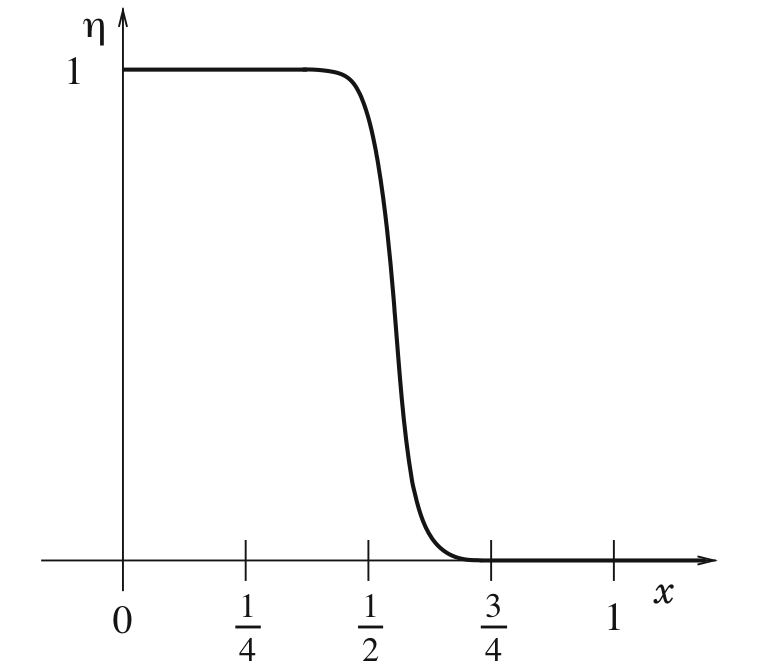
\includegraphics[scale=0.35]{1}
\caption{Function $\eta \left(x\right)$.}
\end{figure}
It follows that $u^{\star} \in W^{1,p}\left(\mathbb{R}\right)$ (see Remark 1.10) and ${\left\| {u^{\star}} \right\|_{{W^{1,p}}\left( \mathbb{R}  \right)}} \le 2{\left\| u \right\|_{{W^{1,p}}\left( I \right)}}$, which is verified as follows.
\begin{align}
{\left\| {u^{\star} } \right\|_{{W^{1,p}}\left( \mathbb{R} \right)}} &= {\left\| {u^{\star} } \right\|_{{L^p}\left( \mathbb{R} \right)}} + {\left\| v \right\|_{{L^p}\left( \mathbb{R} \right)}}\\
 &= {2^{\frac{1}{p}}}\left( {{{\left\| u \right\|}_{{L^p}\left( I \right)}} + {{\left\| {u'} \right\|}_{{L^p}\left( I \right)}}} \right),\mbox{ by \eqref{1.135}}\\
 & = {2^{\frac{1}{p}}}{\left\| u \right\|_{{W^{1,p}}\left( I \right)}}\\
 &\le 2{\left\| u \right\|_{{W^{1,p}}\left( I \right)}}, \mbox{ since } p \ge 1
\end{align}

Now consider the case of a \textit{bounded interval} $I$; without loss of generality we can take $I=\left(0,1\right)$. \textit{Fix} a function $\eta \in C^1\left(\mathbb{R}\right)$, $0\le \eta \le 1$, such that
\begin{align}
\label{1.150}
\eta \left( x \right) = \left\{ {\begin{array}{*{20}{c}}
{1\mbox{ if } x < \frac{1}{4}}\\
{0\mbox{ if } x > \frac{3}{4}}
\end{array}} \right.
\end{align}
See Figure 1.1.

Given a function $f$ on $\left(0,1\right)$ set
\begin{align}
\label{1.151}
\tilde f\left( x \right) = \left\{ {\begin{array}{*{20}{c}}
{f\left( x \right)\mbox{ if } 0 < x < 1}\\
{0\mbox{ if } x > 1}
\end{array}} \right.
\end{align}
We shall need the following lemma.\\
\\
\textbf{Lemma 1.21.} \textit{Let $u \in W^{1,p}\left(I\right)$. Then}
\begin{align}
\label{1.151}
\eta \tilde u &\in {W^{1,p}}\left( {0,\infty } \right)\\
\left( {\eta \tilde u} \right)' &= \eta '\tilde u + \eta \widetilde {u'} \label{1.152}
\end{align}
\textsc{Proof.} Let $\varphi  \in C_c^1\left( {\left( {0,\infty } \right)} \right)$; then
\begin{align}
\int_0^\infty  {\eta \tilde u\varphi '}  &= \int_0^1 {\eta u\varphi '} \\
& = \int_0^1 {u\left( {\left( {\eta \varphi } \right)' - \eta '\varphi } \right)} \\
& =  - \int_0^1 {u'\eta \varphi }  - \int_0^1 {u\eta '\varphi } \mbox{ since } \eta \varphi \in C_c^1\left( {\left( {0,1} \right)} \right)\\
& =  - \int_0^\infty  {\left( {\widetilde {u'}\eta  + \tilde u\eta '} \right)\varphi } 
\end{align}
i.e., \eqref{1.151}-\eqref{1.152} holds. \hfill $\square$\\
\\
\textsc{Proof of Theorem 1.20, concluded.} Given $u\in W^{1,p}\left(I\right)$, write
\begin{align}
u = \eta u + \left( {1 - \eta } \right)u
\end{align}

The function $\eta u$ is \textit{first} extended to $\left(0,\infty\right)$ by $\eta \tilde{u}$ (in view of Lemma 1.21) and \textit{then} to $\mathbb{R}$ by reflexion. In this way we obtain a function $v_1\in W^{1,p}\left(\mathbb{R}\right)$ that extends $\eta u$ and such that
\begin{align}
\label{1.159}
{\left\| {{v_1}} \right\|_{{L^p}\left( \mathbb{R} \right)}} &\le 2{\left\| u \right\|_{{L^p}\left( I \right)}}\\
{\left\| {{v_1}} \right\|_{{W^{1,p}}\left( \mathbb{R} \right)}} &\le C{\left\| u \right\|_{{W^{1,p}}\left( I \right)}} \label{1.160}
\end{align}
(where $C$ depends on ${{{\left\| {\eta '} \right\|}_{{L^\infty }}}}$).\\
\\
\textit{Proof of \eqref{1.159}.} Consider two cases for $p$.
\begin{enumerate}
\item \textit{Case $p=\infty$.} Since $v_1$ is an extension of $\eta \tilde{u}$ obtained by reflexion as $u^{\star}$ is $u$'s extension in the first argument of this proof, we have 
\begin{align}
{\left\| {{v_1}} \right\|_{{L^\infty }\left( \mathbb{R} \right)}} &= {\left\| {\eta \tilde u} \right\|_{{L^\infty }\left( {0,\infty } \right)}}\\
 &= {\left\| {\eta u} \right\|_{{L^\infty }\left( I \right)}}\\
 &\le {\left\| u \right\|_{{L^\infty }\left( I \right)}}\mbox{ since } 0 \le \eta  \le 1
\end{align}
\item \textit{Case $1\le p <\infty$.}
Similarly, we have 
\begin{align}
{\left\| {{v_1}} \right\|_{{L^p}\left( \mathbb{R} \right)}} &= {2^{\frac{1}{p}}}{\left\| {\eta \tilde u} \right\|_{{L^p}\left( {0,\infty } \right)}}\\
& = {2^{\frac{1}{p}}}{\left( {\int_0^{\frac{3}{4}} {{{\left| {\eta \tilde u} \right|}^p}} } \right)^{\frac{1}{p}}},\mbox{ by \eqref{1.150}-\eqref{1.151}}\\
 &\le {2^{\frac{1}{p}}}{\left( {\int_0^{\frac{3}{4}} {{{\left| u \right|}^p}} } \right)^{\frac{1}{p}}}\\
 &\le {2^{\frac{1}{p}}}{\left( {\int_0^1 {{{\left| u \right|}^p}} } \right)^{\frac{1}{p}}}\\
 &\le 2{\left\| u \right\|_{{L^p}\left( I \right)}}\mbox{ since } p \ge 1
\end{align}
\end{enumerate}
\textit{Proof of \eqref{1.160}.}\footnote{The main purpose of this proof is to find such a constant $C$ explicitly.} Similar to the first argument of this proof, we have
\begin{align}
{v_1}'\left( x \right) = \left\{ {\begin{array}{*{20}{c}}
{\left( {\eta \tilde u} \right)'\left( x \right)\mbox{ if } x > 0}\\
{ - \left( {\eta \tilde u} \right)'\left( { - x} \right)\mbox{ if } x < 0}
\end{array}} \right.
\end{align}

We also consider two cases again.
\begin{enumerate}
\item \textit{Case $p=\infty$.} As in the first argument, we have
\begin{align}
{\left\| {{v_1}'} \right\|_{{L^\infty }\left( R \right)}} &= {\left\| {\left( {\eta \tilde u} \right)'} \right\|_{{L^\infty }\left( {0,\infty } \right)}}\\
 &= {\left\| {\eta '\tilde u + \eta \widetilde {u'}} \right\|_{{L^\infty }\left( {0,\infty } \right)}}\\
 &= {\left\| {\eta 'u + \eta u'} \right\|_{{L^\infty }\left( I \right)}}\\
 &\le \max \left\{ {{{\left\| {\eta '} \right\|}_{{L^\infty }}},1} \right\}\left( {{{\left\| u \right\|}_{{L^\infty }\left( I \right)}} + {{\left\| {u'} \right\|}_{{L^\infty }\left( I \right)}}} \right)\\
 &= \max \left\{ {{{\left\| {\eta '} \right\|}_{{L^\infty }}},1} \right\}{\left\| u \right\|_{{W^{1,\infty }}\left( I \right)}}
\end{align}
Thus
\begin{align}
{\left\| {{v_1}} \right\|_{{W^{1,\infty }}\left( \mathbb{R} \right)}} &= {\left\| {{v_1}} \right\|_{{L^\infty }\left( \mathbb{R} \right)}} + {\left\| {{v_1}'} \right\|_{{L^\infty }\left( \mathbb{R} \right)}}\\
& \le {\left\| u \right\|_{{L^\infty }\left( I \right)}} + \max \left\{ {{{\left\| {\eta '} \right\|}_{{L^\infty }}},1} \right\}{\left\| u \right\|_{{W^{1,\infty }}\left( I \right)}}\\
& \le {\left\| u \right\|_{{W^{1,\infty }}\left( I \right)}} + \max \left\{ {{{\left\| {\eta '} \right\|}_{{L^\infty }}},1} \right\}{\left\| u \right\|_{{W^{1,\infty }}\left( I \right)}}\\
& = \left( {1 + \max \left\{ {{{\left\| {\eta '} \right\|}_{{L^\infty }}},1} \right\}} \right){\left\| u \right\|_{{W^{1,\infty }}\left( I \right)}}
\end{align}
Hence, we can choose $C = 1 + \max \left\{ {{{\left\| {\eta '} \right\|}_{{L^\infty }}},1} \right\}$ in \eqref{1.160} when $p=\infty$.
\item \textit{Case $1\le p<\infty$.} Similarly, we have
\begin{align}
\left\| {{v_1}'} \right\|_{{L^p}\left( \mathbb{R} \right)}^p  &= 2\int_0^\infty  {{{\left| {\eta '\tilde u + \eta \widetilde {u'}} \right|}^p}} \\
& = 2\int_0^1 {{{\left| {\eta 'u + \eta u'} \right|}^p}} \\
 &\le 2\int_0^1 {{{\left( {\left| {\eta 'u} \right| + \left| {\eta u'} \right|} \right)}^p}} \\
& \le 2\max \left\{ {\left\| {\eta '} \right\|_{{L^\infty }}^p,1} \right\}\int_0^1 {{{\left( {\left| u \right| + \left| {u'} \right|} \right)}^p}} \\
& \le 2\max \left\{ {\left\| {\eta '} \right\|_{{L^\infty }}^p,1} \right\}\int_0^1 {{2^{p - 1}}\left( {{{\left| u \right|}^p} + {{\left| {u'} \right|}^p}} \right)} \\
& = {2^p}\max \left\{ {\left\| {\eta '} \right\|_{{L^\infty }}^p,1} \right\}{\left\| u \right\|_{{W^{1,p}}\left( I \right)}^p}
\end{align}
where we have used the following familiar elementary inequality
\begin{align}
\label{1.185}
{\left( {a + b} \right)^p} \le {2^{p - 1}}\left( {{{\left| a \right|}^p} + {{\left| b \right|}^p}} \right),\hspace{0.2cm}\forall a,b \in \mathbb{R},\forall p \ge 1
\end{align}
Thus 
\begin{align}
{\left\| {{v_1}} \right\|_{{W^{1,p}}\left( \mathbb{R} \right)}} &= {\left\| {{v_1}} \right\|_{{L^p}\left( \mathbb{R} \right)}} + {\left\| {{v_1}'} \right\|_{{L^p}\left( \mathbb{R} \right)}}\\
& \le 2{\left\| u \right\|_{{L^p}\left( I \right)}} + 2\max \left\{ {{{\left\| {\eta '} \right\|}_{{L^\infty }}},1} \right\}{\left\| u \right\|_{{W^{1,p}}\left( I \right)}}\\
& \le 2{\left\| u \right\|_{{W^{1,p}}\left( I \right)}} + 2\max \left\{ {{{\left\| {\eta '} \right\|}_{{L^\infty }}},1} \right\}{\left\| u \right\|_{{W^{1,p}}\left( I \right)}}\\
& = 2\left( {1 + \max \left\{ {{{\left\| {\eta '} \right\|}_{{L^\infty }}},1} \right\}} \right){\left\| u \right\|_{{W^{1,p}}\left( I \right)}}
\end{align}
Hence, we can choose $C = 2\left( {1 + \max \left\{ {{{\left\| {\eta '} \right\|}_{{L^\infty }}},1} \right\}} \right)$ in \eqref{1.160} when $1\le p<\infty$.
\end{enumerate}

Proceed in the same way with $\left(1-\eta \right)u$, that is, \textit{first} extend $\left(1-\eta \right)u$ to $\left(-\infty,1\right)$ by 0 on $\left(-\infty,0\right)$ and \textit{then} extend to $\mathbb{R}$ by reflection (this time about the point 1, not 0). In this way we obtain a function $v_2\in W^{1,p}\left(\mathbb{R}\right)$ that extends $\left(1-\eta \right)u$ and satisfies
\begin{align}
\label{1.190}
{\left\| {{v_2}} \right\|_{{L^p}\left( \mathbb{R} \right)}} &\le 2{\left\| u \right\|_{{L^p}\left( I \right)}}\\
{\left\| {{v_2}} \right\|_{{W^{1,p}}\left( \mathbb{R} \right)}} &\le C{\left\| u \right\|_{{W^{1,p}}\left( I \right)}} \label{1.191}
\end{align}
\textit{Proof of \eqref{1.190}-\eqref{1.191}.} Similar to \eqref{1.151}, given a function $f$ on $\left(0,1\right)$ set
\begin{align}
\hat f\left( x \right) = \left\{ {\begin{array}{*{20}{c}}
{f\left( x \right)\mbox{ if } 0 < x < 1}\\
{0\mbox{ if } x < 0}
\end{array}} \right.
\end{align}
We shall need the following lemma, which is very similar to Lemma 1.21.\\
\\
\textbf{Lemma 1.22.} \textit{Let $u\in W^{1,p}\left(I\right)$. Then}
\begin{align}
\label{1.193}
\left( {1 - \eta } \right)\hat u &\in {W^{1,p}}\left( { - \infty ,1} \right)\\
\left( {\left( {1 - \eta } \right)\hat u} \right)' &=  - \eta '\hat u + \left( {1 - \eta } \right)\widehat {u'} \label{1.194}
\end{align}
\textit{Proof.} Let $\varphi  \in C_c^1\left( {\left( { - \infty ,1} \right)} \right)$; then
\begin{align}
\int_{ - \infty }^1 {\left( {1 - \eta } \right)\hat u\varphi '}  &= \int_0^1 {\left( {1 - \eta } \right)u\varphi '} \\
& = \int_0^1 {u\left( {\left( {\left( {1 - \eta } \right)\varphi } \right)' - \left( {1 - \eta } \right)'\varphi } \right)} \\
& =  - \int_0^1 {u'\left( {1 - \eta } \right)\varphi }  + \int_0^1 {u\eta '\varphi } \\
& =  - \int_{ - \infty }^1 {\left( {\widehat {u'}\left( {1 - \eta } \right) - \hat u\eta '} \right)\varphi } 
\end{align}
Therefore, \eqref{1.193}-\eqref{1.194} holds. \hfill $\square$\\

Return the the proof of Theorem 1.20, the function $\left(1-\eta \right)u$ is \textit{first} extended to $\left(-\infty,1\right)$ by $\left(1-\eta \right)\hat u$ (in view of Lemma 1.22) and \textit{then} to $\mathbb{R}$ by reflection about the point 1, i.e.,
\begin{align}
{v_2}\left( x \right) = \left\{ {\begin{array}{*{20}{c}}
{\left( {1 - \eta \left( x \right)} \right)\hat u\left( x \right)\mbox{ if } x < 1}\\
{\left( {1 - \eta \left( {2 - x} \right)} \right)\hat u\left( {2 - x} \right)\mbox{ if } x > 1}
\end{array}} \right.
\end{align}

We now prove \eqref{1.190}-\eqref{1.191} as the previous case.\\
\\
\textit{Proof of \eqref{1.190}.} We consider two cases as before.
\begin{enumerate}
\item \textit{Case $p=\infty$.} We have
\begin{align}
{\left\| {{v_2}} \right\|_{{L^\infty }\left( \mathbb{R} \right)}} &= {\left\| {\left( {1 - \eta } \right)\hat u} \right\|_{{L^\infty }\left( { - \infty ,1} \right)}}\\
 &= {\left\| {\left( {1 - \eta } \right)u} \right\|_{{L^\infty }\left( I \right)}}\\
 &\le {\left\| u \right\|_{{L^\infty }\left( I \right)}}
\end{align}
\item \textit{Case $1\le p<\infty$.} Similar to the proof of \eqref{1.159}, we have
\begin{align}
{\left\| {{v_2}} \right\|_{{L^p}\left( \mathbb{R} \right)}} &= {\left( {\int_{ - \infty }^\infty  {{{\left| {{v_2}} \right|}^p}} } \right)^{\frac{1}{p}}}\\
& = {\left( \begin{array}{l}
\int_{ - \infty }^1 {{{\left| {\left( {1 - \eta \left( x \right)} \right)\hat u\left( x \right)} \right|}^p}dx} \\
 + \int_1^\infty  {{{\left| {\left( {1 - \eta \left( {2 - x} \right)} \right)\hat u\left( {2 - x} \right)} \right|}^p}dx} 
\end{array} \right)^{\frac{1}{p}}}\\
& = {\left( \begin{array}{l}
\int_0^1 {{{\left| {\left( {1 - \eta \left( x \right)} \right)\hat u\left( x \right)} \right|}^p}dx} \\
 + \int_{ - \infty }^1 {{{\left| {\left( {1 - \eta \left( t \right)} \right)\hat u\left( t \right)} \right|}^p}dt} 
\end{array} \right)^{\frac{1}{p}}},\mbox{ put } t = 2 - x\\
& = {2^{\frac{1}{p}}}{\left\| {\left( {1 - \eta } \right)u} \right\|_{{L^p}\left( I \right)}}\\
& \le 2{\left\| u \right\|_{{L^p}\left( I \right)}}\mbox{ since } p \ge 1
\end{align}
\end{enumerate}
\textit{Proof of \eqref{1.191}.} We again consider two cases.
\begin{enumerate}
\item \textit{Case $p=\infty$.} As in the first argument, with a light modification, we have
\begin{align}
{\left\| {{v_2}'} \right\|_{{L^\infty }\left( \mathbb{R} \right)}} &= {\left\| {\left( {\left( {1 - \eta } \right)\hat u} \right)'} \right\|_{{L^\infty }\left( { - \infty ,1} \right)}}\\
& = {\left\| { - \eta '\hat u + \left( {1 - \eta } \right)\widehat {u'}} \right\|_{{L^\infty }\left( { - \infty ,1} \right)}},\mbox{ by \eqref{1.194}}\\
& = {\left\| { - \eta 'u + \left( {1 - \eta } \right)u'} \right\|_{{L^\infty }\left( I \right)}}\\
& \le \max \left\{ {{{\left\| {\eta '} \right\|}_{{L^\infty }}},1} \right\}\left( {{{\left\| u \right\|}_{{L^\infty }\left( I \right)}} + {{\left\| {u'} \right\|}_{{L^\infty }\left( I \right)}}} \right)\\
& = \max \left\{ {{{\left\| {\eta '} \right\|}_{{L^\infty }}},1} \right\}{\left\| u \right\|_{{W^{1,\infty }}\left( I \right)}}
\end{align}
Thus
\begin{align}
{\left\| {{v_2}} \right\|_{{W^{1,\infty }}\left( \mathbb{R} \right)}} &= {\left\| {{v_2}} \right\|_{{L^\infty }\left( \mathbb{R} \right)}} + {\left\| {{v_2}'} \right\|_{{L^\infty }\left( \mathbb{R} \right)}}\\
& \le {\left\| u \right\|_{{L^\infty }\left( I \right)}} + \max \left\{ {{{\left\| {\eta '} \right\|}_{{L^\infty }}},1} \right\}{\left\| u \right\|_{{W^{1,\infty }}\left( I \right)}}\\
& \le \left( {1 + \max \left\{ {{{\left\| {\eta '} \right\|}_{{L^\infty }}},1} \right\}} \right){\left\| u \right\|_{{W^{1,\infty }}\left( I \right)}}
\end{align}
Hence, we can again choose $C = 1 + \max \left\{ {{{\left\| {\eta '} \right\|}_{{L^\infty }}},1} \right\}$ in \eqref{1.191} when $p=\infty$.
\item \textit{Case $\le p<\infty$.} We have
\begin{align}
\left\| {{v_2}'} \right\|_{{L^p}\left( \mathbb{R}  \right)}^p &= 2\int_{ - \infty }^1 {{{\left| { - \eta '\hat u + \left( {1 - \eta } \right)\widehat {u'}} \right|}^p}} \\
 &= 2\int_0^1 {{{\left| { - \eta 'u + \left( {1 - \eta } \right)u'} \right|}^p}} \\
& \le 2\int_0^1 {{{\left( {\left| {\eta 'u} \right| + \left| {\left( {1 - \eta } \right)u'} \right|} \right)}^p}} \\
& \le 2\max \left\{ {\left\| {\eta '} \right\|_{{L^\infty }}^p,1} \right\}\int_0^1 {{{\left( {\left| u \right| + \left| {u'} \right|} \right)}^p}} \\
& \le {2^p}\max \left\{ {\left\| {\eta '} \right\|_{{L^\infty }}^p,1} \right\}\int_0^1 {\left( {{{\left| u \right|}^p} + {{\left| {u'} \right|}^p}} \right)} \\
& = {2^p}\max \left\{ {\left\| {\eta '} \right\|_{{L^\infty }}^p,1} \right\}\left\| u \right\|_{{W^{1,p}}\left( I \right)}^p
\end{align}
where we again use \eqref{1.185}. Hence, 
\begin{align}
{\left\| {{v_2}} \right\|_{{W^{1,p}}\left( \mathbb{R}  \right)}} &= {\left\| {{v_2}} \right\|_{{L^p}\left( \mathbb{R}  \right)}} + {\left\| {{v_2}'} \right\|_{{L^p}\left( \mathbb{R}  \right)}}\\
 &\le 2{\left\| u \right\|_{{L^p}\left( I \right)}} + 2\max \left\{ {{{\left\| {\eta '} \right\|}_{{L^\infty }}},1} \right\}{\left\| u \right\|_{{W^{1,p}}\left( I \right)}}\\
 &\le 2{\left\| u \right\|_{{W^{1,p}}\left( I \right)}} + 2\max \left\{ {{{\left\| {\eta '} \right\|}_{{L^\infty }}},1} \right\}{\left\| u \right\|_{{W^{1,p}}\left( I \right)}}\\
& = 2\left( {1 + \max \left\{ {{{\left\| {\eta '} \right\|}_{{L^\infty }}},1} \right\}} \right){\left\| u \right\|_{{W^{1,p}}\left( I \right)}}
\end{align}
Hence, we can choose $C = 2\left( {1 + \max \left\{ {{{\left\| {\eta '} \right\|}_{{L^\infty }}},1} \right\}} \right)$ in \eqref{1.191} when $1\le p<\infty$.
\end{enumerate}

Return to the proof of Theorem 1.20, then $PU=v_1 +v_2$ satisfies the condition of the theorem. More explicitly, we have
\begin{align}
{\left. {Pu} \right|_I} = u,\hspace{0.2cm}\forall u \in {W^{1,p}}\left( I \right),1 \le p \le \infty 
\end{align}
and
\begin{enumerate}
\item For $p=\infty$, 
\begin{align}
\label{1.227}
{\left\| {Pu} \right\|_{{L^\infty }\left( \mathbb{R} \right)}} &\le 2{\left\| u \right\|_{{L^\infty }\left( I \right)}}\\
{\left\| {Pu} \right\|_{{W^{1,\infty }}\left( \mathbb{R} \right)}} &\le 2\left( {1 + \max \left\{ {{{\left\| {\eta '} \right\|}_{{L^\infty }}},1} \right\}} \right){\left\| u \right\|_{{W^{1,\infty }}\left( I \right)}}
\end{align}
for all $u \in {W^{1,\infty }}\left( I \right)$.
\item For $1\le p<\infty$,
\begin{align}
{\left\| {Pu} \right\|_{{L^p}\left( \mathbb{R} \right)}} &\le 4{\left\| u \right\|_{{L^p}\left( I \right)}}\\
{\left\| {Pu} \right\|_{{W^{1,p}}\left( \mathbb{R} \right)}} &\le 4\left( {1 + \max \left\{ {{{\left\| {\eta '} \right\|}_{{L^\infty }}},1} \right\}} \right){\left\| u \right\|_{{W^{1,p}}\left( I \right)}} \label{1.230}
\end{align}
for all $u \in {W^{1,p}}\left( I \right)$. 
\end{enumerate}
With some suitable choices of $\eta$, \eqref{1.227}-\eqref{1.230} will be more easy to use. \hfill $\square$\\

Certain properties of $C^1$ functions remain true for $W^{1,p}$ functions (see for example Corollaries 8.10 and 8.11, \cite{1}). It is convenient to establish these properties by a \textit{density} argument based on the following result.\\
\\
\textbf{Theorem 1.23 (density).} \textit{Le $u\in W^{1,p}\left(I\right)$ with $1\le p<\infty$. Then there exists a sequence $\left(u_n\right)$ in $C_c^{\infty}\left(\mathbb{R}\right)$ such that ${\left. {{u_n}} \right|_I} \to u$ in $W^{1,p}\left(I\right)$.}\\
\\
\textbf{Remark 1.24.} In general, there is no sequence $\left(u_n\right)$ in $C_c^{\infty}\left(I\right)$ such that $u_n\to u$ in $W^{1,p}\left(I\right)$ (See Section 1.3). This is contrast to $L^p$ spaces: recall that for every function $u\in L^p\left(I\right)$ there s a sequence $\left(u_n\right)$ in $C_c^{\infty}\left(I\right)$ such that $u_n\to u$ in $L^p\left(I\right)$ (see Corollary 4.23, \cite{1}).\\
\\
\textsc{Proof.} We can always suppose $I=\mathbb{R}$; otherwise, extend $u$ to a function in $W^{1,p}\left(\mathbb{R}\right)$ by Theorem 1.20. We use the \textit{basic techniques of convolution} (which makes functions $C^{\infty}$) and \textit{cut-off} (which makes their support compact).\\
\\
\textbf{(a) Convolution.}

We shall need the following lemma.\\
\\
\textbf{Lemma 1.25.} \textit{Let $\rho \in L^1\left(\mathbb{R}\right)$ and $v\in W^{1,p}\left(\mathbb{R}\right)$ with $1\le p\le \infty$. Then $\rho \star v \in W^{1,p}\left(\mathbb{R}\right)$ and $\left(p\star v\right)'=\rho \star v'$.}\\
\\
\textsc{Proof.} First, suppose that $\rho$ has compact support. We already know (Theorem 4.15, \cite{1}) that $\rho \star v\in L^p\left(\mathbb{R}\right)$. Let $\varphi \in C_c^1\left(\mathbb{R}\right)$; from Propositions 4.16 and 4.20, \cite{1}, we have
\begin{align}
\int {\left( {\rho \star v} \right)\varphi '}  &= \int {v\left( {\mathord{\buildrel{\lower3pt\hbox{$\scriptscriptstyle\smile$}} 
\over \rho } \star \varphi '} \right)} \\
 &= \int {v\left( {\mathord{\buildrel{\lower3pt\hbox{$\scriptscriptstyle\smile$}} 
\over \rho } \star \varphi } \right)'} \\
& =  - \int {v'\left( {\mathord{\buildrel{\lower3pt\hbox{$\scriptscriptstyle\smile$}} 
\over \rho } \star \varphi } \right)} \\
& =  - \int {\left( {\rho \star v'} \right)\varphi } 
\end{align}
from which it follows that
\begin{align}
\rho \star v &\in {W^{1,p}}\\
\left( {\rho \star v} \right)' &= \rho \star v'
\end{align}
If $\rho$ does not have compact support introduce a sequence $\left(\rho _n\right)$ from $C_c\left(\mathbb{R}\right)$ such that $\rho _n\to \rho $ in $L^1\left(\mathbb{R}\right)$ (see Corollary 4.23). From the above, we get
\begin{align}
\rho _n\star v &\in {W^{1,p}}\\
\left( {\rho _n \star v} \right)' &= \rho _n \star v'
\end{align}
But $\rho _n\star v \to \rho \star v$ in $L^p\left(\mathbb{R}\right)$ and $\rho _n\star v' \to \rho \star v'$ in $L^p\left(\mathbb{R}\right)$ (by Theorem 4.15, \cite{1}). We conclude with the help of Remark 1.9 that
\begin{align}
\rho \star v &\in {W^{1,p}}\\
\left( {\rho \star v} \right)' &= \rho \star v'
\end{align}
\textbf{(b) Cut-off.}

\textit{Fix} a function $\zeta  \in C_c^\infty \left( \mathbb{R} \right)$ such that $0\le \zeta \le 1$ and
\begin{align}
\zeta \left( x \right) = \left\{ {\begin{array}{*{20}{c}}
{1\mbox{ if } \left| x \right| < 1}\\
{0\mbox{ if } \left| x \right| \ge 2}
\end{array}} \right.
\end{align}
Define the sequence
\begin{align}
{\zeta _n}\left( x \right) = \zeta \left( {\frac{x}{n}} \right)\mbox{ for } n = 1,2, \ldots 
\end{align}
It follows easily from the dominated convergence theorem that if a function $f$ belongs to $L^p\left(\mathbb{R}\right)$ with $1\le p<\infty$, then $\zeta _nf\to f$ in $L^p\left(\mathbb{R}\right)$.\\
\\
\textbf{(c) Conclusion.} 

Choose a sequence of mollifiers $\left(\rho _n\right)$. We claim that the sequence ${u_n} = {\zeta _n}\left( {{\rho _n}\star u} \right)$ converges to $u$ in $W^{1,p}\left(\mathbb{R}\right)$. First, we have ${\left\| {{u_n} - u} \right\|_p} \to 0$. In fact, write
\begin{align}
{u_n} - u = {\zeta _n}\left( {\left( {{\rho _n}\star u} \right) - u} \right) + \left( {{\zeta _n}u - u} \right)
\end{align}
and thus
\begin{align}
\label{1.244}
{\left\| {{u_n} - u} \right\|_p} &\le {\left\| {{\zeta _n}\left( {\left( {{\rho _n}\star u} \right) - u} \right)} \right\|_p} + {\left\| {{\zeta _n}u - u} \right\|_p}\\
& \le {\left\| {{\zeta _n}} \right\|_{\infty}}{\left\| {\left( {{\rho _n}\star u} \right) - u} \right\|_p} + {\left\| {{\zeta _n}u - u} \right\|_p}\\
& = {\left\| {\left( {{\rho _n}\star u} \right) - u} \right\|_p} + {\left\| {{\zeta _n}u - u} \right\|_p} \to 0 \label{1.246}
\end{align}
where we have use the following inequality
\begin{align}
{\left\| {fg} \right\|_p} \le {\left\| f \right\|_\infty }{\left\| g \right\|_p},\hspace{0.2cm} \forall f \in C_c^\infty \left( \mathbb{R} \right),\hspace{0.2cm} \forall g \in {L^p}\left( \mathbb{R} \right)
\end{align}
Next, by Lemma 1.25, we have
\begin{align}
{u_n}' = {\zeta _n}'\left( {{\rho _n}\star u} \right) + {\zeta _n}\left( {{\rho _n}\star u'} \right)
\end{align}
Therefore
\begin{align}
\label{1.249}
{\left\| {{u_n}' - u'} \right\|_p} &= {\left\| {{\zeta _n}'\left( {{\rho _n}\star u} \right) + {\zeta _n}\left( {{\rho _n}\star u'} \right) - u'} \right\|_p}\\
& \le {\left\| {{\zeta _n}'\left( {{\rho _n}\star u} \right)} \right\|_p} + {\left\| {{\zeta _n}\left( {{\rho _n}\star u'} \right) - u'} \right\|_p}\\
& \le {\left\| {{\zeta _n}'} \right\|_\infty }{\left\| {{\rho _n}\star u} \right\|_p} + {\left\| {{\zeta _n}\left( {{\rho _n}\star u' - u'} \right)} \right\|_p} + {\left\| {{\zeta _n}u' - u'} \right\|_p}\\
& \le \frac{C}{n}{\left\| {{\rho _n}} \right\|_1}{\left\| u \right\|_p} + {\left\| {{\zeta _n}} \right\|_\infty }{\left\| {{\rho _n}\star u' - u'} \right\|_p} + {\left\| {{\zeta _n}u' - u'} \right\|_p}\\
& = \frac{C}{n}{\left\| u \right\|_p} + {\left\| {{\rho _n}\star u' - u'} \right\|_p} + {\left\| {{\zeta _n}u' - u'} \right\|_p} \to 0 \label{1.253}
\end{align}
where $C = {\left\| {\zeta '} \right\|_\infty }$.

Combining \eqref{1.244}-\eqref{1.246} and \eqref{1.249}-\eqref{1.253} yields
\begin{align}
{\left\| {{u_n} - u} \right\|_{{W^{1,p}}\left( \mathbb{R} \right)}} = {\left\| {{u_n} - u} \right\|_{{L^p}\left( \mathbb{R} \right)}} + {\left\| {{u_n}' - u'} \right\|_{{L^p}\left( R \right)}} \to 0
\end{align}
i.e., $\left(u_n\right)$ is a desired sequence. \hfill $\square$\\

The next result is an important prototype of a \textit{Sobolev inequality} (also called a \textit{Sobolev embedding}).\\
\\
\textbf{Theorem 1.26.} \textit{There exists a constant $C$ (depending only on $\left| I \right| \le \infty $) such that}
\begin{align}
\label{1.255}
{\left\| u \right\|_{{L^\infty }\left( I \right)}} \le C{\left\| u \right\|_{{W^{1,p}}\left( I \right)}},\hspace{0.2cm}\forall u \in {W^{1,p}}\left( I \right),\hspace{0.2cm}\forall 1 \le p \le \infty 
\end{align}
\textit{In other words, ${W^{1,p}}\left( I \right) \subset {L^\infty }\left( I \right)$ with continuous injection for all $1\le p\le \infty$.}

\textit{Further, if $I$ is \textbf{bounded} then}
\begin{enumerate}
\item \textit{The \textbf{injection} ${W^{1,p}}\left( I \right) \subset C\left( {\bar I} \right)$ is \textbf{compact} for all $1<p\le \infty$.}
\item \textit{The \textbf{injection} ${W^{1,1}}\left( I \right) \subset {L^q}\left( I \right)$ is \textbf{compact} for all $1\le q< \infty$.}
\end{enumerate}
\textsc{Proof.} We start by proving \eqref{1.255} for $I=\mathbb{R}$; the general case then follows from this by the extension theorem (Theorem 1.20). 

The case $p=\infty$ is obvious since
\begin{align}
{\left\| u \right\|_\infty } &\le {\left\| u \right\|_\infty } + {\left\| {u'} \right\|_\infty }\\
 &= {\left\| u \right\|_{{W^{1,\infty }}}},\hspace{0.2cm}\forall u \in {W^{1,\infty }}\left( R \right)
\end{align}
It now suffices to prove \eqref{1.255} for $1\le p<\infty$.  

Let $v\in C_c^1\left(\mathbb{R}\right)$; if $1\le p <\infty$ set $G\left( s \right) = {\left| s \right|^{p - 1}}s$. The function $w=G\left(v\right)$ belongs to $C_c^1\left(\mathbb{R}\right)$ and\footnote{\eqref{1.257} can be easily verified by considering two cases $v\ge 0$ and $v <0$.}
\begin{align}
w' &= G'\left( v \right)v'\\
 &= p{\left| v \right|^{p - 1}}v' \label{1.257}
\end{align}
Thus, for $x\in \mathbb{R}$, we have
\begin{align}
G\left( {v\left( x \right)} \right) = \int_{ - \infty }^x {p{{\left| {v\left( t \right)} \right|}^{p - 1}}v'\left( t \right)dt} 
\end{align}
and by H\"{o}lder's inequality
\begin{align}
\label{1.259}
{\left| {v\left( x \right)} \right|^p} &= \left| {G\left( {v\left( x \right)} \right)} \right|\\
& = \left| {\int_{ - \infty }^x {p{{\left| {v\left( t \right)} \right|}^{p - 1}}v'\left( t \right)dt} } \right|\\
& \le p{\left\| {{v^{p - 1}}v'} \right\|_{_1}}\\
& \le p{\left\| {{v^{p - 1}}} \right\|_{\frac{p}{{p - 1}}}}{\left\| {v'} \right\|_p}\mbox{ by H\"{o}lder's}\\
& = p{\left( {\int_{\mathbb{R}} {{{\left| {{v^{p - 1}}} \right|}^{\frac{p}{{p - 1}}}}} } \right)^{\frac{{p - 1}}{p}}}{\left\| {v'} \right\|_p}\\
& = p\left\| v \right\|_p^{p - 1}{\left\| {v'} \right\|_p} \label{1.264}
\end{align}
from which we conclude that
\begin{align}
\label{1.267}
{\left\| v \right\|_\infty } \le C{\left\| v \right\|_{{W^{1,p}}}},\hspace{0.2cm}\forall v \in C_c^1\left( \mathbb{R} \right)
\end{align}
where $C$ is a universal constant (independent of $p$).\footnote{Noting that ${p^{\frac{1}{p}}} \le {e^{\frac{1}{e}}},\hspace{0.2cm}\forall p \ge 1$.}\\
\\ 
\textit{Proof of \eqref{1.267}.} We consider three cases.
\begin{enumerate}
\item \textit{Case $p=1$.} In this case, \eqref{1.259}-\eqref{1.264} becomes
\begin{align}
\left| {v\left( x \right)} \right| \le {\left\| {v'} \right\|_1}
\end{align}
Thus
\begin{align}
{\left\| v \right\|_\infty } &\le {\left\| {v'} \right\|_1}\\
& \le {\left\| v \right\|_1} + {\left\| {v'} \right\|_1}\\
& = {\left\| v \right\|_{{W^{1,p}}}},\hspace{0.2cm}\forall v \in C_c^1\left( \mathbb{R} \right)
\end{align}
Therefore, we can choose $C=1$ in \eqref{1.267} when $p=1$.
\item \textit{Case $1<p<\infty$.} To this end, we need the following inequality.
\begin{align}
\label{1.272}
1 + x \ge p{\left( {\frac{x}{{{{\left( {p - 1} \right)}^{p - 1}}}}} \right)^{\frac{1}{p}}},\hspace{0.2cm}\forall p > 1,\hspace{0.2cm}\forall x > 0
\end{align}
To prove \eqref{1.272}, we rewrite it as follows.
\begin{align}
\label{1.273}
\frac{{{{\left( {p - 1} \right)}^{p - 1}}{{\left( {1 + x} \right)}^p}}}{{{p^p}x}} \ge 1,\hspace{0.2cm}\forall p > 1,\hspace{0.2cm}\forall x > 0
\end{align}
Taking natural logarithm of both sides of \eqref{1.273}, it suffices to prove
\begin{align}
\left( {p - 1} \right)\ln \left( {p - 1} \right) + p\ln \left( {1 + x} \right) \ge p\ln p + \ln x,\hspace{0.2cm}\forall p > 1,\hspace{0.2cm}\forall x > 0
\end{align}
Surveying the following function
\begin{align}
f\left( p \right) = \left( {p - 1} \right)\ln \left( {p - 1} \right) + p\ln \left( {1 + x} \right) - p\ln p - \ln x ,
\end{align}
for all $p>1$ and for all $x>0$, yields
\begin{align}
f'\left( p \right) &= \ln \left( {p - 1} \right) + \ln \left( {1 + x} \right) - \ln p\\
f'\left( p \right) = 0 &\Leftrightarrow p = 1 + \frac{1}{x}\\
f''\left( p \right) &= \frac{1}{{p\left( {p - 1} \right)}} > 0
\end{align}
Hence, 
\begin{align}
&\mathop {\min }\limits_{p > 1} f\left( p \right)\\
 &= f\left( {1 + \frac{1}{x}} \right)\\
& = \frac{1}{x}\ln \frac{1}{x} - \left( {1 + \frac{1}{x}} \right)\ln \left( {1 + \frac{1}{x}} \right) - \ln x + \left( {1 + \frac{1}{x}} \right)\ln \left( {x + 1} \right)\\
& =  - \frac{1}{x}\ln x + \left( {1 + \frac{1}{x}} \right)\ln \left( {\frac{x}{{x + 1}}} \right) - \ln x + \left( {1 + \frac{1}{x}} \right)\ln \left( {x + 1} \right)\\
& =  - \left( {1 + \frac{1}{x}} \right)\ln x + \left( {1 + \frac{1}{x}} \right)\left( {\ln \left( {\frac{x}{{x + 1}}} \right) + \ln \left( {x + 1} \right)} \right)\\
& =  - \left( {1 + \frac{1}{x}} \right)\ln x + \left( {1 + \frac{1}{x}} \right)\ln x\\
 &= 0
\end{align}
Thus, \eqref{1.272} holds. 

Return to our proof of \eqref{1.267}, we can suppose that ${\left\| v \right\|_p} > 0,{\left\| {v'} \right\|_p} > 0$ since there is nothing to prove on the other cases. Substituting $x = \frac{{{{\left\| {v'} \right\|}_p}}}{{{{\left\| v \right\|}_p}}} >0$ into \eqref{1.272} yields
\begin{align}
{\left\| v \right\|_p} + {\left\| {v'} \right\|_p} &\ge p{\left( {\frac{{\left\| v \right\|_p^{p - 1}{{\left\| {v'} \right\|}_p}}}{{{{\left( {p - 1} \right)}^{p - 1}}}}} \right)^{\frac{1}{p}}}\\
& \ge p{\left( {\frac{{{{\left| {v\left( x \right)} \right|}^p}}}{{p{{\left( {p - 1} \right)}^{p - 1}}}}} \right)^{\frac{1}{p}}}\\
& = {\left( {\frac{p}{{p - 1}}} \right)^{\frac{{p - 1}}{p}}}\left| {v\left( x \right)} \right|\\
& \ge \left| {v\left( x \right)} \right|
\end{align}
i.e., 
\begin{align}
{\left\| v \right\|_\infty } \le {\left\| v \right\|_{{W^{1,p}}}},\hspace{0.2cm}\forall v \in C_c^1\left( \mathbb{R} \right),\hspace{0.2cm} 1<p<\infty
\end{align}
Therefore, we can also choose $C=1$ in \eqref{1.267} when $1<p< \infty$.
\end{enumerate}

Argue now by density. Let $u\in W^{1,p}\left(\mathbb{R}\right)$; there exists a sequence $\left(u_n\right)\subset C_c^1\left(\mathbb{R}\right)$ such that $u_n\to u$ in $W^{1,p}\left(\mathbb{R}\right)$ (by Theorem 1.23). Applying \eqref{1.267}, we see that $\left(u_n\right)$ is a Cauchy sequence in $L^{\infty}\left(\mathbb{R}\right)$. Indeed, 
\begin{align}
{\left\| {{u_m} - {u_n}} \right\|_\infty } &\le C{\left\| {{u_m} - {u_n}} \right\|_{{W^{1,p}}}},\mbox{ by \eqref{1.267}}\\
 &\le C\left( {{{\left\| {{u_m} - u} \right\|}_{{W^{1,p}}}} + {{\left\| {u - {u_n}} \right\|}_{{W^{1,p}}}}} \right) \to 0
\end{align}
as $m,n\to \infty$.

Thus $u_n\to u$ in $L^{\infty}\left(\mathbb{R}\right)$ and we obtain \eqref{1.255}.\\
\\
\textit{Proof of $\left(1\right)$.} Let $\mathcal{H}$ be the unit ball in $W^{1,p}\left(I\right)$ with $1<p\le \infty$. For $u\in \mathcal{H}$ we have
\begin{align}
\label{1.293}
\left| {u\left( x \right) - u\left( y \right)} \right| &= \left| {\int_x^y {u'\left( t \right)dt} } \right|\\
 &\le {\left\| {u'} \right\|_p}{\left\| 1 \right\|_{p'}},\mbox{ by Holder's inequality}\\
 &= {\left\| {u'} \right\|_p}{\left| {x - y} \right|^{\frac{1}{{p'}}}},\mbox{ by }{\left\| u \right\|_{{W^{1,p}}\left( I \right)}} \le 1\\
& \le {\left| {x - y} \right|^{\frac{1}{{p'}}}} \label{1.296}
\end{align}
It follows then from the Ascoli-Arzel\`{a} theorem (Theorem 4.25, \cite{1}) that $\mathcal{H}$ has a compact closure in $C\left(\bar{I}\right)$. 

Indeed, applying Ascoli-Arzel\`{a} theorem to the compact metric space $\left( {\bar I,\left|  \cdot  \right|} \right)$, where ${\left|  \cdot  \right|}$ is usual Euclidean distance in the real number line, and the bounded subset $H = {B_{{W^{1,p}}\left( I \right)}}\left( {0,1} \right)$ of $C\left( {\bar I} \right)$. It is deduced from \eqref{1.293}-\eqref{1.296} that $\mathcal{H}$ is uniformly equicontinuous. More explicitly, given $\varepsilon >0$, we have
\begin{align}
\left| {x - y} \right| < {\varepsilon ^{p'}} \Rightarrow \left| {u\left( x \right) - u\left( y \right)} \right| < \varepsilon ,\hspace{0.2cm}\forall u \in \mathcal{H}
\end{align}
Then, by Ascoli-Arzel\`{a} theorem, the closure of $\mathcal{H}$ in $C\left(\bar{I}\right)$ is compact. By definition of compact operator (Section 6.1, \cite{1}), $\left(1\right)$ holds.\\
\\
\textsc{Proof of $\left(2\right)$.} Let $\mathcal{H}$ be the unit ball in $W^{1,1}\left(I\right)$. Let $P$ be the extension operator of Theorem 1.20 and set $\mathcal{F}=P\left(\mathcal{H}\right)$, so that $\mathcal{H} = {\mathcal{F}_{\left| I \right.}}$. We prove that $\mathcal{H}$ has a compact closure in $L^q\left(I\right)$ (for all $1 \le q<\infty$) by applying Theorem 4.26 (Kolmogorov - M. Riesz - Fr\'{e}chet), \cite{1}. Clearly, $\mathcal{F}$ is bounded in $W^{1,1}\left(\mathbb{R}\right)$\footnote{See the proof of Theorem 1.20.}; therefore $\mathcal{F}$ is also bounded in $L^q\left(\mathbb{R}\right)$, since it is bounded both in $L^1\left(\mathbb{R}\right)$ and in $L^{\infty}\left(\mathbb{R}\right)$. We now check the following condition
\begin{align}
\mathop {\lim }\limits_{h \to 0} {\left\| {{\tau _h}f - f} \right\|_q} = 0\mbox{ uniformly in } f  \in \mathcal{F}
\end{align}
By Proposition 1.19\footnote{Note that the implication $\left(1\right) \Rightarrow \left(2\right)$ of Theorem 1.19 is also valid when $p=1$.} we have, for every $f\in \mathcal{F}$,
\begin{align}
{\left\| {{\tau _h}f - f} \right\|_{{L^1}\left( \mathbb{R} \right)}} &\le \left| h \right|{\left\| {f'} \right\|_{{L^1}\left(\mathbb{R} \right)}}\\
 &\le C\left| h \right|
\end{align}
since $\mathcal{F}$ is a bounded subset of $W^{1,1}\left(\mathbb{R}\right)$. Thus
\begin{align}
\left\| {{\tau _h}f - f} \right\|_{{L^q}\left( {\mathbb{R}} \right)}^q &= \int_{\mathbb{R}} {{{\left| {{\tau _h}f - f} \right|}^q}} \\
& = \int_{\mathbb{R}} {{{\left| {f\left( {x + h} \right) - f\left( x \right)} \right|}^{q - 1}}\left| {{\tau _h}f - f} \right|dx} \\
& \le {\left( {2{{\left\| f \right\|}_{{L^\infty }\left( {\mathbb{R}} \right)}}} \right)^{q - 1}}{\left\| {{\tau _h}f - f} \right\|_{{L^1}\left( {\mathbb{R}} \right)}}\\
&\le C\left| h \right|
\end{align}
and consequently
\begin{align}
\label{1.305}
{\left\| {{\tau _h}f - f} \right\|_{{L^q}\left( \mathbb{R} \right)}} \le C_0{\left| h \right|^{\frac{1}{q}}}
\end{align}
where $C$ is independent of $f$. The desired conclusion follows since $q\ne \infty$.

Indeed, given $\varepsilon >0$, it is deduced from \eqref{1.305} that
\begin{align}
{\left\| {{\tau _h}f - f} \right\|_{{L^q}\left( \mathbb{R} \right)}} < \varepsilon ,\hspace{0.2cm}\forall f \in F,\hspace{0.2cm}\forall h \in \mathbb{R},\left| h \right| < \frac{{{\varepsilon ^q}}}{{C_0^q}}
\end{align}
We then deduce, by applying Kolmogorov- M. Riesz-Fr\'{e}chet theorem, that the closure of ${\mathcal{F}_{\left| I \right.}}$ in $L^q\left(I\right)$ is compact for the bounded measurable set $I$. Hence, by definition of compact operator again, $\left(2\right)$ holds. \hfill $\square$\\
\\
\textbf{Remark 1.27.} The origin of the inequality \eqref{1.272} is given by the following idea. Look at the case $p \in {\mathbb{Z}_ + }\backslash \left\{ 1 \right\}$, we can use Cauchy inequality for $p$ nonnegative numbers
\begin{align}
{\left\| v \right\|_{{W^{1,p}}}} &= {\left\| v \right\|_p} + {\left\| {v'} \right\|_p}\\
& = \underbrace {\frac{{{{\left\| v \right\|}_p}}}{{p - 1}} +  \cdots  + \frac{{{{\left\| v \right\|}_p}}}{{p - 1}}}_{\left( {p - 1} \right)'s} + {\left\| {v'} \right\|_p}\\
& \ge p{\left( {\frac{{\left\| v \right\|_p^{p - 1}{{\left\| {v'} \right\|}_p}}}{{{{\left( {p - 1} \right)}^{p - 1}}}}} \right)^{\frac{1}{p}}}\mbox{ by Cauchy's inequality}\\
& \ge p{\left( {\frac{{{{\left| {v\left( x \right)} \right|}^p}}}{{p{{\left( {p - 1} \right)}^{p - 1}}}}} \right)^{\frac{1}{p}}}\\
& = {\left( {\frac{p}{{p - 1}}} \right)^{\frac{{p - 1}}{p}}}\left| {v\left( x \right)} \right|\\
& \ge \left| {v\left( x \right)} \right|
\end{align}
Roughly speaking, \eqref{1.272} is an extended version of this estimation for arbitrary real number $p>1$. But proving \eqref{1.272} requires a little more calculus skills than just applying Cauchy inequality here, of course.\\
\\
\textbf{Remark 1.28.} The injection $W^{1,1}\left(I\right) \subset C\left(\bar{I}\right)$ is continuous but it is \textit{never compact}, even if $I$ is a bounded interval. Nevertheless, if $\left(u_n\right)$ is a bounded sequence in $W^{1,1}\left(I\right)$ (with $I$ bounded or unbounded) there exists a subsequence $\left(u_{n_k}\right)$ such that $u_{n_k}\left(x\right)$ converges for \textit{all} $x\in I$ (this is \textit{Helly's selection theorem}). When $I$ is \textit{unbounded} and $1<p\le \infty$, we know that the injection $W^{1,p}\left(I\right)\subset L^{\infty}\left(I\right)$ is continuous; this injection is \textit{never compact}. However, if $\left(u_n\right)$ is bounded in $W^{1,p}\left(I\right)$ with $1<p\le \infty$ there exist a subsequence $\left(u_{n_k}\right)$ and some $u\in W^{1,p}\left(I\right)$ such that $u_{n_k}\to u$ in $L^{\infty}\left(I\right)$ for every \textit{bounded} subset $J$ of $I$.\\
\\
\textbf{Remark 1.29.} Let $I$ be a bounded interval, let $1\le p\le \infty$, and let $1\le q\le \infty$. From Theorem 1.10 and \eqref{1.255} it can be shown easily that the norm
\begin{align}
|||u||| = {\left\| {u'} \right\|_p} + {\left\| u \right\|_q}
\end{align}
is equivalent to the norm of $W^{1,p}\left(I\right)$.\\
\\
\textsc{Proof of Remark 1.29.} Consider the following cases.
\begin{enumerate}
\item \textit{Case $p=q$ (including the case $p=\infty,q=\infty$).} The conclusion is obvious since $||| \cdot ||| \equiv {\left\|  \cdot  \right\|_{{W^{1,p}}\left( I \right)}}$.
\item \textit{Case $p\ne q$. }
\begin{enumerate}
\item \textit{Case $1 \le p < q = \infty $.} We have
\begin{align}
|||u||| &= {\left\| {u'} \right\|_p} + {\left\| u \right\|_\infty }\\
& \le {\left\| {u'} \right\|_p} + C{\left\| u \right\|_{{W^{1,p}}\left( I \right)}}\\
& \le \left( {1 + C} \right){\left\| u \right\|_{{W^{1,p}}\left( I \right)}}
\end{align}
On the other hand,
\begin{align}
{\left\| u \right\|_{{W^{1,p}}\left( I \right)}} &= {\left\| {u'} \right\|_p} + {\left\| u \right\|_p}\\
& \le {\left\| {u'} \right\|_p} + {\left| I \right|^{\frac{1}{p}}}{\left\| u \right\|_\infty }\\
& \le \max \left\{ {1,{{\left| I \right|}^{\frac{1}{p}}}} \right\}|||u|||
\end{align}
\item \textit{Case $1 \le p < q < \infty$.} We have
\begin{align}
|||u||| &= {\left\| {u'} \right\|_p} + {\left\| u \right\|_q}\\
& \le {\left\| {u'} \right\|_p} + {\left\| u \right\|_{{L^\infty }\left( I \right)}}{\left\| 1 \right\|_q}\\
& = {\left\| {u'} \right\|_p} + {\left\| u \right\|_{{L^\infty }\left( I \right)}}{\left| I \right|^{\frac{1}{q}}}\\
& \le {\left\| {u'} \right\|_p} + C{\left| I \right|^{\frac{1}{q}}}{\left\| u \right\|_{{W^{1,p}}\left( I \right)}},\mbox{ by \eqref{1.255}}\\
& \le \left( {1 + C{{\left| I \right|}^{\frac{1}{q}}}} \right){\left\| u \right\|_{{W^{1,p}}\left( I \right)}}
\end{align}
On the other hand, we have
\begin{align}
{\left\| u \right\|_{{W^{1,p}}\left( I \right)}} &= {\left\| u \right\|_p} + {\left\| {u'} \right\|_p}\\
 &= \left\| {{u^p}} \right\|_1^{\frac{1}{p}} + {\left\| {u'} \right\|_p}\\
& \le {\left( {{{\left\| {{u^p}} \right\|}_{\frac{q}{p}}}{{\left\| 1 \right\|}_{\frac{q}{{q - p}}}}} \right)^{\frac{1}{p}}} + {\left\| {u'} \right\|_p}\\
& = {\left\| u \right\|_q}{\left| I \right|^{\frac{1}{p} - \frac{1}{q}}} + {\left\| {u'} \right\|_p}\\
& \le \max \left\{ {{{\left| I \right|}^{\frac{1}{p} - \frac{1}{q}}},1} \right\}\left( {{{\left\| u \right\|}_q} + {{\left\| {u'} \right\|}_p}} \right)\\
& = \max \left\{ {{{\left| I \right|}^{\frac{1}{p} - \frac{1}{q}}},1} \right\}|||u|||
\end{align} 
Reader should notice that the condition $1\le p<q<\infty$ guarantees $1 < \frac{q}{{q - p}} < \infty $.
\item \textit{Case $1 \le q < p = \infty $.} 
\item \textit{Case $1\le q<p<\infty$.}\footnote{Hoang Cong Duc's proof.} We have
\begin{align}
\label{1.331}
{\left\| u \right\|_p} &\le \left\| u \right\|_\infty ^{\frac{{p - q}}{p}}\left\| u \right\|_q^{\frac{q}{p}}\\
& = {k^{\frac{{p - q}}{p}}}{\left( {\frac{{{{\left\| u \right\|}_\infty }}}{k}} \right)^{\frac{{p - q}}{p}}}\left\| u \right\|_q^{\frac{q}{p}},\hspace{0.2cm} k > 0\mbox{ is chosen later}\\
& \le \frac{{{k^{\frac{{p - q}}{p}}}}}{p}\left( {\frac{{p - q}}{k}{{\left\| u \right\|}_\infty } + q{{\left\| u \right\|}_q}} \right)\\
 &\le \frac{{{k^{\frac{{p - q}}{p}}}}}{p}\left( {\frac{{C\left( {p - q} \right)}}{k}\left( {{{\left\| {u'} \right\|}_p} + {{\left\| u \right\|}_p}} \right) + q{{\left\| u \right\|}_q}} \right)\label{1.334}
\end{align}
We now choose ${k^{ - \frac{q}{p}}}\frac{{C\left( {p - q} \right)}}{p} < 1$, for instance, let $k$ satisfy
\begin{align}
{k^{ - \frac{q}{p}}}\frac{{C\left( {p - q} \right)}}{p} = \frac{1}{2}
\end{align}
then \eqref{1.331}-\eqref{1.334} works.
\end{enumerate}
\end{enumerate}
\textbf{Remark 1.30.} Let $I$ be an \textit{unbounded} interval. If $u\in W^{1,p}\left(I\right)$, then $u\in L^q\left(I\right)$ for all $q\in \left[p,\infty\right]$, since
\begin{align}
\int_I {{{\left| u \right|}^q}}  \le \left\| u \right\|_\infty ^{q - p}\left\| u \right\|_p^p
\end{align}
But in general $u \notin {L^q}\left( I \right)$ for $q \in \left[1,p\right)$. (Why?)\\
\\
\textbf{Corollary 1.31.} \textit{Suppose that $I$ is an unbounded interval and $u\in W^{1,p}\left(I\right)$ with $1\le p<\infty$. Then}
\begin{align}
\label{1.336}
\mathop {\lim }\limits_{x \in I,\left| x \right| \to \infty } u\left( x \right) = 0
\end{align}
\textsc{Proof.} From Theorem 1.23 there exists a sequence $\left(u_n\right)$ in $C_c^1\left(\mathbb{R}\right)$ such that ${u_{\left. n \right|I}} \to u$ in $W^{1,p}\left(I\right)$. It follows from \eqref{1.255} that 
\begin{align}
{\left\| {{u_n} - u} \right\|_{{L^\infty }\left( I \right)}} \le C{\left\| {{u_n} - u} \right\|_{{W^{1,p}}\left( I \right)}} \to 0
\end{align}
as $n \to \infty $. We deduce \eqref{1.336} from this. Indeed, given $\varepsilon >0$ we choose $n$ large enough that ${\left\| {{u_n} - u} \right\|_{{L^\infty }\left( I \right)}} < \varepsilon $. For $\left| x \right|$ large enough, $u_n\left(x\right)=0$ (since $u_n\in C_c^1\left(\mathbb{R}\right)$) and thus $\left| {u\left( x \right)} \right| < \varepsilon $.\\
\\
\textbf{Corollary 1.32 (differentiation of a product).}\footnote{Note the \textit{contrast} of this result with the properties of $L^p$ functions: in general, if $u,v\in L^p$, the product $uv$ does \textit{not} belong to $L^p$. (Why?) We say that $W^{1,p}\left(I\right)$ is a \textit{Banach algebra}.} \textit{Let $u,v\in W^{1,p}\left(I\right)$ with $1\le p\le \infty$. Then} 
\begin{align}
uv \in {W^{1,p}}\left( I \right)
\end{align}
\textit{and}
\begin{align}
\label{1.339}
\left( {uv} \right)' = u'v + uv'
\end{align}
\textit{Furthermore, the formula for integration by parts holds}
\begin{align}	
\label{1.337}
\int_y^x {u'v}  = u\left( x \right)v\left( x \right) - u\left( y \right)v\left( y \right) - \int_y^x {uv'} ,\hspace{0.2cm}\forall x,y \in \bar I
\end{align}
\textsc{Proof.} First call that $u\in L^{\infty}$ (by Theorem 1.26) and thus $uv\in L^p$.\footnote{Indeed, $\int_I {{{\left| {uv} \right|}^p}}  \le {\left\| u \right\|_\infty }\int_I {{{\left| v \right|}^p}}  < \infty $ since $u\in L^{\infty}$ and $v\in L^p$.} To show that $\left(uv\right)'\in L^p$ let us begin with the case $1\le p<\infty$. Let $\left(u_n\right)$ and $\left(v_n\right)$ be sequences in $C_c^1\left(\mathbb{R}\right)$ such that ${u_{\left. n \right|I}} \to u$ and ${v_{\left. n \right|I}} \to v$ in $W^{1,p}\left(I\right)$. Thus ${u_{\left. n \right|I}} \to u$ and ${v_{\left. n \right|I}} \to v$ in $L^{\infty}\left(I\right)$ (again by Theorem 1.26). It follows that ${u_n}{v_{\left. n \right|I}} \to uv$ in $L^{\infty}\left(I\right)$ and also in $L^p$. 

Indeed, to prove that ${u_n}{v_{\left. n \right|I}} \to uv$ in $L^{\infty}\left(I\right)$, using Minkowski's in equality yields
\begin{align}
&{\left\| {{u_n}{v_{\left. n \right|I}} - uv} \right\|_\infty } \\
&= {\left\| {u\left( {{v_{\left. n \right|I}} - v} \right) + {v_{\left. n \right|I}}\left( {{u_{\left. n \right|I}} - u} \right)} \right\|_\infty }\\
 &\le {\left\| u \right\|_\infty }{\left\| {{v_{\left. n \right|I}} - v} \right\|_\infty } + {\left\| {{v_{\left. n \right|I}}} \right\|_\infty }{\left\| {{u_{\left. n \right|I}} - u} \right\|_\infty }\\
 &\le C\left( {{{\left\| u \right\|}_\infty }{{\left\| {{v_{\left. n \right|I}} - v} \right\|}_{{W^{1,p}}\left( I \right)}} + {{\left\| {{v_{\left. n \right|I}}} \right\|}_\infty }{{\left\| {{u_{\left. n \right|I}} - u} \right\|}_{{W^{1,p}}\left( I \right)}}} \right) \to 0
\end{align}
as $n \to \infty $ since 
\begin{align}
\label{1.345}
{\left\| {{v_{\left. n \right|I}}} \right\|_\infty } \le C{\left\| {{v_{\left. n \right|I}}} \right\|_{{W^{1,p}}\left( I \right)}} \to C{\left\| v \right\|_{{W^{1,p}}\left( I \right)}}\mbox{ as } n \to \infty 
\end{align}
which is bounded as $n \to \infty $. 

Similarly, to prove ${u_n}{v_{\left. n \right|I}} \to uv$ in $L^p\left(I\right)$, using Minkowski's in equality again yields
\begin{align}
&{\left\| {{u_n}{v_{\left. n \right|I}} - uv} \right\|_p} \\
&= {\left\| {u\left( {{v_{\left. n \right|I}} - v} \right) + {v_{\left. n \right|I}}\left( {{u_{\left. n \right|I}} - u} \right)} \right\|_p}\\
& \le {\left\| {u\left( {{v_{\left. n \right|I}} - v} \right)} \right\|_p} + {\left\| {{v_{\left. n \right|I}}\left( {{u_{\left. n \right|I}} - u} \right)} \right\|_p}\\
& \le \left\| u \right\|_\infty ^{\frac{1}{p}}{\left\| {{v_{\left. n \right|I}} - v} \right\|_p} + \left\| {{v_{\left. n \right|I}}} \right\|_\infty ^{\frac{1}{p}}{\left\| {{u_{\left. n \right|I}} - u} \right\|_p}\\
& \le \left\| u \right\|_\infty ^{\frac{1}{p}}{\left\| {{v_{\left. n \right|I}} - v} \right\|_{{W^{1,p}}\left( I \right)}} + \left\| {{v_{\left. n \right|I}}} \right\|_\infty ^{\frac{1}{p}}{\left\| {{u_{\left. n \right|I}} - u} \right\|_{{W^{1,p}}\left( I \right)}} \to 0
\end{align}
as $n \to \infty$, where ${\left\| {{v_{\left. n \right|I}}} \right\|_\infty }$ is handled as \eqref{1.345}. We have
\begin{align}
\left( {{u_n}{v_n}} \right)' = {u_n}'{v_n} + {u_n}{v_n}' \to u'v + uv'\mbox{ in } {L^p}\left( I \right)
\end{align}
Applying once more Remark 1.9 to the sequence $\left(u_nv_n\right)$, we conclude that $uv\in W^{1,p}\left(I\right)$ and that \eqref{1.339} holds. Integrating \eqref{1.339}, we obtain \eqref{1.337}.

We now turn to the case $p=\infty$; let $u,v\in W^{1,\infty}\left(I\right)$. Thus $uv\in L^{\infty}\left(I\right)$ and $u'v+uv'\in L^{\infty}\left(I\right)$. It remains to check that
\begin{align}
\int_I {uv\varphi '}  =  - \int_I {\left( {u'v + uv'} \right)\varphi } ,\hspace{0.2cm}\forall \varphi  \in C_c^1\left( I \right)
\end{align}
For this, fix a bounded open interval $J\subset I$ such that $\mbox{supp } \varphi \subset J$. Thus $u,v\in W^{1,p}\left(J\right)$ for all $p<\infty$ and from the above we know that
\begin{align}
\int_J {uv\varphi '}  =  - \int_J {\left( {u'v + uv'} \right)\varphi } 
\end{align}
that is,
\begin{align}
\int_I {uv\varphi '}  =  - \int_I {\left( {u'v + uv'} \right)\varphi } 
\end{align}
\textbf{Corollary 1.33 (differentiation of a composition).} \textit{Let $G \in C^1\left(\mathbb{R}\right)$ be such that\footnote{This restriction is unnecessary when $I$ is bounded (or also if $I$ is unbounded and $p=\infty$). It is essential if $I$ is unbounded and $1\le p<\infty$ (Why?).} $G\left(0\right)=0$, and let $u\in W^{1,p}\left(I\right)$ with $1\le p \le \infty$. Then}
\begin{align}
G \circ u &\in {W^{1,p}}\left( I \right)\\
\left( {G \circ u} \right)' &= \left( {G' \circ u} \right)u'
\end{align}
\textsc{Proof.} Let $M = {\left\| u \right\|_\infty }$. We have $M<\infty$ since $u\in W^{1,p}\left(I\right)$ and \eqref{1.255}. Since $G\left(0\right)=0$, there exists a constant $C$ such that $\left| {G\left( s \right)} \right| \le C\left| s \right|$ for all $s\in \left[-M,+M\right]$. Thus $\left| {G \circ u} \right| \le C\left| u \right|$ ; it follows that $G \circ u \in {L^p}\left( I \right)$ . Similarly, $\left( {G' \circ u} \right)u' \in {L^p}\left( I \right)$. Indeed, since $G' \in C\left(\mathbb{R}\right)$, there exists a constant $C_1$ such that $\left| {G'\left( s \right) - G'\left( 0 \right)} \right| \le {C_1}\left| s \right|$ for all $s\in \left[-M,+M\right]$. Hence,
\begin{align}
\left| {G'\left( {u\left( x \right)} \right)} \right| &\le {C_1}\left| {u\left( x \right)} \right| + \left| {G'\left( 0 \right)} \right|\\
 &\le {C_1}{\left\| u \right\|_\infty } + \left| {G'\left( 0 \right)} \right|
\end{align}
Thus
\begin{align}
\left| {\left( {G' \circ u} \right)u'} \right| \le {C_1}{\left\| u \right\|_\infty }\left| {u'} \right| + \left| {G'\left( 0 \right)} \right|\left| {u'} \right|
\end{align}
which immediately implies that $\left( {G' \circ u} \right)u' \in {L^p}\left( I \right)$ as stated. 

It remains to verify that
\begin{align}
\label{1.360}
\int_I {\left( {G \circ u} \right)\varphi '}  =  - \int_I {\left( {G' \circ u} \right)u'\varphi } ,\hspace{0.2cm}\forall \varphi  \in C_c^1\left( I \right)
\end{align}
Suppose first that $1\le p<\infty$. Then there exists a sequence $\left(u_n\right)$ from $C_c^1\left(\mathbb{R}\right)$ such that ${u_{\left. n \right|I}} \to u$ in $W^{1,p}\left(I\right)$ and also in $L^{\infty}\left(I\right)$. Thus ${\left( {G \circ {u_n}} \right)_{|I}} \to G \circ u$ in $L^{\infty}\left(I\right)$ and $\left( {G' \circ u} \right){u_{\left. n \right|I}}' \to \left( {G' \circ u} \right)u'$ in $L^p\left(I\right)$. Clearly (by the standard rules for $C^1$ functions) we have
\begin{align}
\int_I {\left( {G \circ {u_n}} \right)\varphi '}  =  - \int_I {\left( {G' \circ {u_n}} \right){u_n}'\varphi } ,\hspace{0.2cm} \forall \varphi  \in C_c^1\left( I \right)
\end{align}
from which we deduce \eqref{1.360}. For the case $p=\infty$ proceed in the same manner as in the proof of Corollary 1.32. More explicitly, fix a bounded open interval $J\subset I$ such that $\mbox{supp }\varphi \subset J$. Thus $u\in W^{1,p}\left(J\right)$ for all $p<\infty$ and by \eqref{1.360} we know that
\begin{align}
\int_J {\left( {G \circ u} \right)\varphi '}  =  - \int_J {\left( {G' \circ u} \right)u'\varphi } 
\end{align}
that is,
\begin{align}
\int_I {\left( {G \circ u} \right)\varphi '}  =  - \int_I {\left( {G' \circ u} \right)u'\varphi } 
\end{align}
This completes our proof. \hfill $\square$
\section*{The Sobolev Spaces $W^{m,p}$.}
\textbf{Definition 1.34.} Given an integer $m\ge 2$ and a real number $1\le p\le \infty$ we define by induction the space
\begin{align}
{W^{m,p}}\left( I \right) = \left\{ {u \in {W^{m - 1,p}}\left( I \right);u' \in {W^{m - 1,p}}\left( I \right)} \right\}
\end{align}
We also set
\begin{align}
{H^m}\left( I \right) = {W^{m,2}}\left( I \right)
\end{align}
It is easily shown  (Why?)that $u\in W^{m,p}\left(I\right)$ if and only if there exist $m$ functions $g_1,\ldots,g_m\in L^p\left(I\right)$ such that
\begin{align}
\int_I {u{D^j}\varphi }  = {\left( { - 1} \right)^j}\int_I {{g_j}\varphi } ,\hspace{0.2cm}\forall \varphi  \in C_c^\infty \left( I \right), \hspace{0.2cm}\forall j = 1,2, \ldots ,m
\end{align}
where $D^j \varphi$ denotes the $j$th derivative of $\varphi$. When $u\in W^{m,p}\left(I\right)$ we may thus consider the successive derivatives of $u$: $u' = {g_1},\left( {u'} \right)' = {g_2}, \ldots $, up to order $m$. They are denoted by $Du,D^2u,\ldots,D^mu$. The space $W^{m,p}\left(I\right)$ is equipped with the norm
\begin{align}
{\left\| u \right\|_{{W^{m,p}}}} = {\left\| u \right\|_p} + \sum\limits_{\alpha  = 1}^m {{{\left\| {{D^\alpha }u} \right\|}_p}} 
\end{align}
and the space $H^m\left(I\right)$ is equipped with the scalar product
\begin{align}
{\left( {u,v} \right)_{{H^m}}} &= {\left( {u,v} \right)_{{L^2}}} + \sum\limits_{\alpha  = 1}^m {{{\left( {{D^\alpha }u,{D^\alpha }v} \right)}_{{L^2}}}} \\
& = \int_I {uv}  + \sum\limits_{\alpha  = 1}^m {\int_I {{D^\alpha }u{D^\alpha }v} } 
\end{align}
One can show that the norm ${\left\|  \cdot  \right\|_{{W^{m,p}}}}$ is equivalent to the norm
\begin{align}
|||u||| = {\left\| u \right\|_p} + {\left\| {{D^m}u} \right\|_p}
\end{align}
\textsc{Proof of the equivalent of ${\left\|  \cdot  \right\|_{{W^{m,p}}}}$ and $|||\cdot|||$.}  (Why?)\\
\\
More precisely, one proves that for every integer $j$, $1\le j\le m-1$, and for every $\varepsilon >0$ there exists a constant $C$ (depending on $\varepsilon$ and $\left| I \right| \le \infty $)  such that
\begin{align}
{\left\| {{D^j}u} \right\|_p} \le \varepsilon {\left\| {{D^m}u} \right\|_p} + C{\left\| u \right\|_p},\hspace{0.2cm}\forall u \in {W^{m,p}}\left( I \right)
\end{align}
( (Why?)see Exercise 8.6, \cite{1} for the case $\left| I \right| < \infty $).

The reader can extend to the space $W^{m,p}$ all the properties shown for $W^{1,p}$; for example, if $I$ is bounded, $W^{m,p}\left(I\right) \subset C^{m-1}\left(\bar{I}\right)$ with continuous injection (resp. compact injection for $1<p\le \infty)$.
\section{The Space $W_0^{1,p}$} 
\textbf{Definition 1.35.} Given $1\le p<\infty$, denote by $W_0^{1,p}\left(I\right)$ the closure of $C_c^1\left(I\right)$ in $W^{1,p}\left(I\right)$.\footnote{We doe not define $W_0^{1,p}$ for $p=\infty$.} Set
\begin{align}
H_0^1\left( I \right) = W_0^{1,2}\left( I \right)
\end{align}
The space $W_0^{1,2}\left(I\right)$ is equipped with the norm of $W^{1,p}\left(I\right)$, and the space $H_0^1$ is equipped with the scalar product of $H^1$.\footnote{When there is no confusion we often write $W_0^{1,p}$ and $H_0^1$ instead of $W_0^{1,p}\left(I\right)$ and $H_0^1\left(I\right)$.}

The space $W_0^{1,p}$ is a separable Banach space. Moreover, it is reflexive for $p>1$. The space $H_0^1$ is a separable Hilbert space.\\
\\
\textbf{Remark 1.36.} When $I=\mathbb{R}$ we know that $C_c^1\left(\mathbb{R}\right)$ is dense in $W^{1,p}\left(\mathbb{R}\right)$ (see Theorem 1.23) and therefore $W_0^{1,p}\left(\mathbb{R}\right)=W^{1,p}\left(\mathbb{R}\right)$.\\
\\
\textbf{Remark 1.37.} Using a sequence of mollifiers $\left(\rho _n\right)$ it is easy to check the following: (Why?)
\begin{enumerate}
\item $C_c^{\infty}$ is dense in $W_0^{1,p}\left(I\right)$.
\item If $u \in {W^{1,p}}\left( I \right) \cap {C_c}\left( I \right)$ then $u\in W_0^{1,p}\left(I\right)$. 
\end{enumerate}

Our next result provides a basic characterization of functions in $W_0^{1,p}\left(I\right)$.\\
\\
\textbf{Theorem 1.38.} \textit{Let $u\in W^{1,p}\left(I\right)$. Then $u\in W_0^{1,p}\left(I\right)$ if and only if $u=0$ on $\partial I$.}\\
\\
\textbf{Remark 1.39.} Theorem 1.38 explains the central role played by the space $W_0^{1,p}\left(I\right)$. Differential equations (or partial differential equations) are often coupled with \textit{boundary conditions}, i.e., the value of $u$ is prescribed on $\partial I$.\\
\\
\textsc{Proof of Theorem 1.38.} If $u\in W_0^{1,p}$, there exists a sequence $\left(u_n\right)$ in $C_c^1\left(I\right)$ such that $u_n\to u$ in $W^{1,p}\left(I\right)$ (by definition of $W_0^{1,p}$. Therefore $u_n\to u$ uniformly on $\bar{I}$  \footnote{Indeed, by \eqref{1.255}, 
\begin{align}
{\left\| {{u_n} - u} \right\|_{{L^\infty }\left( {\bar I} \right)}} &= {\left\| {{u_n} - u} \right\|_{{L^\infty }\left( I \right)}}\\
 &\le C{\left\| {{u_n} - u} \right\|_{{W^{1,p}}\left( I \right)}} \to 0
\end{align}
as $n\to \infty$, where the first equality is deduced by the fact that $\partial I$ has zero measure.} and as a consequence $u=0$ on $\partial I$ ($u_n=0$ on $\partial I$).

\textit{Conversely}, let $u\in W^{1,p}\left(I\right)$ be such that $u=0$ on $\partial I$. Fix any function $G\in C^1\left(\mathbb{R}\right)$ such that
\begin{align}
G\left( t \right) = \left\{ {\begin{array}{*{20}{c}}
{0\mbox{ if } \left| t \right| \le 1}\\
{t\mbox{ if } \left| t \right| \ge 2}
\end{array}} \right.
\end{align}
and
\begin{align}
\left| {G\left( t \right)} \right| \le \left| t \right|,\hspace{0.2cm}\forall t \in \mathbb{R}
\end{align}
Set ${u_n} = \frac{1}{n}G\left( {nu} \right)$, so that $u_n\in W^{1,p}\left(I\right)$ (by Corollary 1.33). On the other hand,
\begin{align}
\mbox{supp }{u_n} \subset \left\{ {x \in I;\left| {u\left( x \right)} \right| \ge \frac{1}{n}} \right\}
\end{align}
and thus $\mbox{supp }u_n$ is in a compact subset of $I$ (using the fact that $u=0$ on $\partial I$ and $u\left(x\right)\to 0$ as $\left| x \right| \to \infty ,x \in I$, see Corollary 1.31). Therefore $u_n\in W_0^{1,p}\left(I\right)$ (Why?) (see Remark 1.37). Finally, one easily checks that $u_n\to u$ in $W^{1,p}\left(I\right)$ by the dominated convergence theorem.  (Why?)(dominated convergence theorem for $L^p$) Thus $u\in W_0^{1,p}\left(I\right)$. \hfill $\square$\\
\\
\textbf{Remark 1.40.} Let us mention two other characterizations of $W_0^{1,p}$ functions:
\begin{enumerate}
\item Let $1\le p<\infty$ and let $u\in L^p\left(I\right)$. Define $\bar{u}$ by
\begin{align}
\bar u\left( x \right) = \left\{ {\begin{array}{*{20}{l}}
{u\left( x \right)\mbox{ if } x \in I}\\
{0\hspace{0.6cm}\mbox{ if } x \in \mathbb{R} \backslash I}
\end{array}} \right.
\end{align}
Then $u\in W_0^{1,p}\left(I\right)$ if and only if $\bar u \in W^{1,p}\left(\mathbb{R}\right)$. (Why?)
\item Let $1<p<\infty$ and let $u\in L^p\left(I\right)$. Then $u$ belongs to $W_0^{1,p}\left(I\right)$ if and only if there exists a constant $C$ such that (Why?)
\begin{align}
\left| {\int_I {u\varphi '} } \right| \le C{\left\| \varphi  \right\|_{{L^{p'}}\left( I \right)}},\hspace{0.2cm}\forall \varphi  \in C_c^1\left( \mathbb{R} \right)
\end{align}
\end{enumerate}
\textbf{Proposition 1.41 (Poincar\'{e}'s inequality).} \textit{Suppose $I$ is a \textbf{bounded} interval. Then there exists a constant $C$ (depending on $\left| I \right| < \infty $) such that}
\begin{align}
\label{1.377}
{\left\| u \right\|_{{W^{1,p}}\left( I \right)}} \le C{\left\| {u'} \right\|_{{L^p}\left( I \right)}},\hspace{0.2cm}\forall u \in W_0^{1,p}\left( I \right) 
\end{align} 
\textit{In other words, on $W_0^{1,p}$, the quantity ${\left\| {u'} \right\|_{{L^p}\left( I \right)}}$ is a norm equivalent to the $W^{1,p}$ norm.}\\
\\
\textsc{Proof.} Let $u \in W_0^{1,p}\left( I \right)$ (with $I=\left(a,b\right)$). Since $u\left(a\right)=0$, we have
\begin{align}
\left| {u\left( x \right)} \right| &= \left| {u\left( x \right) - u\left( a \right)} \right|\\
& = \left| {\int_a^x {u'\left( t \right)dt} } \right|\\
& \le \int_a^x {\left| {u'\left( t \right)} \right|dt} \\
& \le \int_a^b {\left| {u'\left( t \right)} \right|dt} \\
& = {\left\| {u'} \right\|_{{L^1}\left(I\right)}}
\end{align}
Thus ${\left\| u \right\|_{{L^\infty }\left( I \right)}} \le {\left\| {u'} \right\|_{{L^1}\left( I \right)}}$ and \eqref{1.377} then follows by H\"{o}lder's inequality. More explicitly,
\begin{align}
{\left\| u \right\|_{{W^{1,p}}\left( I \right)}} &= {\left\| u \right\|_p} + {\left\| {u'} \right\|_p}\\
& \le {\left| I \right|^{\frac{1}{p}}}{\left\| u \right\|_\infty } + {\left\| {u'} \right\|_p}\\
& \le {\left| I \right|^{\frac{1}{p}}}{\left\| {u'} \right\|_{{L^1}\left( I \right)}} + {\left\| {u'} \right\|_p}\\
& \le {\left| I \right|^{\frac{1}{p}}}{\left| I \right|^{\frac{1}{{p'}}}}{\left\| {u'} \right\|_p} + {\left\| {u'} \right\|_p}\\
& = \left( {\left| I \right| + 1} \right){\left\| {u'} \right\|_p}
\end{align}
Thus, we can take ${C = \left| I \right| + 1}$ in \eqref{1.377}. \hfill $\square$\\
\\
\textbf{Remark 1.42.} If $I$ is bounded, the expression ${\left( {u',v'} \right)_{{L^2}}} = \int_I {u'v'} $ defines a scalar product on $H_0^1$ and the associated norm, i.e., ${\left\| {u'} \right\|_{{L^2}}}$, is equivalent to the $H^1$ norm.
\begin{align}
{\left\| {u'} \right\|_{{L^2}\left( I \right)}} \le {\left\| u \right\|_{{H^1}\left( I \right)}} \le C{\left\| {u'} \right\|_{{L^2}\left( I \right)}},\hspace{0.2cm}\forall u \in H_0^1\left( I \right)
\end{align}
\textbf{Remark 1.43.} Given an integer $m\ge 2$ and a real number $1\le p<\infty$, the space $W_0^{m,p}\left(I\right)$ is defined as the closure of $C_c^m\left(I\right)$ in $W^{m,p}\left(I\right)$. Once shows (see Exercise 8.9, \cite{1}) that
\begin{align}
W_0^{m,p}\left( I \right) = \left\{ {u \in {W^{m,p}}\left( I \right);u = Du =  \cdots  = {D^{m - 1}}u = 0\mbox{ on } \partial I} \right\}
\end{align}
It is essential to notice the \textit{distinction} between
\begin{align}
W_0^{2,p}\left( I \right) = \left\{ {u \in {W^{2,p}}\left( I \right);u = Du = 0\mbox{ on } \partial I} \right\}
\end{align}
and
\begin{align}
{W^{2,p}}\left( I \right) \cap W_0^{1,p}\left( I \right) = \left\{ {u \in {W^{2,p}}\left( I \right);u = 0\mbox{ on } \partial I} \right\}
\end{align}
\section*{The Dual Space of $W_0^{1,p}\left(I\right)$}
\textbf{Notation.} The dual space of $W_0^{1,p}\left(I\right)$ ($1\le p<\infty$) is denoted by ${W^{ - 1,p'}}\left( I \right)$ and the dual space of $H_0^1\left(I\right)$ is denoted by $H^{-1}\left(I\right)$. 

Following Remark 3 of Chapter 5, \cite{1}, \textit{we identify $L^2$ and its dual, but we do not identify $H_0^1$ and its dual.} We have the inclusions (Why?)
\begin{align}
H_0^1 \subset {L^2} \subset {H^{ - 1}}
\end{align}
where these injections are continuous and dense (i.e., they have dense ranges). 

If $I$ is a bounded interval we have
\begin{align}
W_0^{1,p} \subset {L^2} \subset {W^{ - 1,p'}},\hspace{0.2cm}\forall 1 \le p \le 2
\end{align}
with continuous injections (see Remark 1.30).

The elements of $W^{-1,p'}$ can be represented with the help of functions in $L^{p'}$; to be precise, we have the following\\
\\
\textbf{Proposition 1.44.} \textit{Let $F\in W^{-1,p'}\left(I\right)$. Then there exist two functions $f_0,f_1\in L^{p'}\left(I\right)$ such that}
\begin{align}
\left\langle {F,u} \right\rangle  = \int_I {{f_0}u}  + \int_I {{f_1}u'} ,\hspace{0.2cm}\forall u \in W_0^{1,p}\left( I \right)
\end{align}
\textit{and}
\begin{align}
{\left\| F \right\|_{{W^{ - 1,p'}}}} = \max \left\{ {{{\left\| {{f_0}} \right\|}_{p'}},{{\left\| {{f_1}} \right\|}_{p'}}} \right\}
\end{align}
\textit{When $I$ is \textbf{bounded} we can take $f_0=0$.}\\
\\
\textsc{Proof.} Consider the product space $E=L^p\left(I\right)\times L^p\left(I\right)$ equipped with the norm
\begin{align}
\left\| h \right\| = {\left\| {{h_0}} \right\|_p} + {\left\| {{h_1}} \right\|_p}\mbox{ where } h = \left[ {{h_0},{h_1}} \right]
\end{align}
The map $T:u \in W_0^{1,p}\left( I \right) \mapsto \left[ {u,u'} \right] \in E$ is an isometry from $W_0^{1,p}\left(I\right)$ into $E$. Set $G = T\left( {W_0^{1,p}\left( I \right)} \right)$ equipped with the norm of $E$ and $S = {T^{ - 1}}:G \to W_0^{1,p}\left( I \right)$. The map $h \in G \mapsto \left\langle {F,Sh} \right\rangle $ is a continuous linear functional on $G$. By the Hahn-Banach theorem, it can be extended to a continuous linear function $\Phi $ on all of $E$ with ${\left\| \Phi  \right\|_{{E^{\star}}}} = \left\| F \right\|$. By the Riesz representation theorem we know that there exist two functions $f_0,f_1\in L^{p'}\left(I\right)$ such that
\begin{align}
\left\langle {\Phi ,h} \right\rangle  = \int_I {{f_0}{h_0}}  + \int_I {{f_1}{h_1}} ,\hspace{0.2cm}\forall h = \left[ {{h_0},{h_1}} \right] \in E
\end{align}
It is easy to check that (Why?) ${\left\| \Phi  \right\|_{{E^{\star}}}} = \max \left\{ {{{\left\| {{f_0}} \right\|}_{p'}},{{\left\| {{f_1}} \right\|}_{p'}}} \right\}$. Also, we have
\begin{align}
\left\langle {\Phi ,Tu} \right\rangle  = \left\langle {F,u} \right\rangle  = \int_I {{f_0}u}  + \int_I {{f_1}u'} ,\hspace{0.2cm}\forall u \in W_0^{1,p}\left( I \right)
\end{align}
When $I$ is \textit{bounded} the space $W_0^{1,p}\left(I\right)$ may be equipped with the norm ${\left\| {u'} \right\|_p}$ (see Proposition 1.41). We repeat  (Why?) the same argument with $E=L^p\left(I\right)$ and $T:u \in {W^{1,p}}\left( I \right) \mapsto u' \in {L^p}\left( I \right)$. \hfill $\square$\\
\\
\textbf{Remark 1.45.} The functions $f_0$ and $f_1$ are not uniquely determined by $F$.\\
\\
\textbf{Remark 1.46.} The element $F\in W^{-1,p'}\left(I\right)$ is usually identified with the distribution $f_0-f_1'$ (by definition, the distribution $f_0-f_1'$ is the linear functional $u \mapsto \int_I {{f_0}u}  + \int_I {{f_1}u'} $, on $C_c^{\infty} \left(I\right)$).\\
\\
\textbf{Remark 1.47.}  (Why?)The first assertion of Proposition  1.44 also holds for continuous linear functionals on $W^{1,p}$ ($1\le p<\infty$), i.e., every continuous linear functional $F$ on $W^{1,p}$ may be represented as
\begin{align}
\left\langle {F,u} \right\rangle  = \int_I {{f_0}u}  + \int_I {{f_1}u'} ,\hspace{0.2cm}\forall u \in {W^{1,p}}
\end{align}
for some functions $f_0,f_1\in L^{p'}$.
\section{Some Examples of Boundary Value Problems}
Consider the problem
\begin{align}
\label{1.400}
 - u'' + u &= f\mbox{ on } I = \left( {0,1} \right)\\
u\left( 0 \right) &= u\left( 1 \right) = 0 \label{1.401}
\end{align}
where $f$ is a given function (for example in $C\left(\bar I\right)$ or more generally in $L^2\left(I\right)$). \textit{The boundary condition $u\left(0\right)=u\left(1\right)=0$} is called the (homogeneous) \textit{Dirichlet boudnary condition}.\\
\\
\textbf{Definition 1.48.} A \textit{classical solution} of \eqref{1.400}-\eqref{1.401} is a function $u\in C^2\left(\bar I\right)$ satisfying \eqref{1.400}-\eqref{1.401} in the usual sense. A \textit{weak solution} of \eqref{1.400}-\eqref{1.401} is a function $u\in H_0^1\left(I\right)$ satisfying
\begin{align}
\label{1.402}
\int_I {u'v'}  + \int_I {uv}  = \int_I {fv} ,\hspace{0.2cm}\forall v \in H_0^1\left( I \right)
\end{align}

Let us ``put in action'' the program outlined in Section 1.1:\\
\\
\textbf{Step A. Every classical solution is a weak solution.} This is obvious by integration by parts (as justified in Corollary 1.32). Indeed, multiplying both sides of \eqref{1.400} with $v\in H_0^1\left(I\right)$ gives
\begin{align}
\label{1.403}
 - \int_I {u''v}  + \int_I {uv}  = \int_I {fv} ,\hspace{0.2cm}\forall v \in H_0^1\left( I \right)
\end{align}
Using integration by parts formula \eqref{1.337} gives
\begin{align}
\label{1.404}
 - \int_I {u''v}  &=  - u'\left( 1 \right)v\left( 1 \right) + u'\left( 0 \right)v\left( 0 \right) + \int_I {u'v'} \\
& = \int_I {u'v'}  ,\hspace{0.2cm}\forall v \in H_0^1\left( I \right) \label{1.405}
\end{align}
since $v\left(0\right)=v\left(1\right)=0$. Combining \eqref{1.403} with \eqref{1.404}-\eqref{1.405} yields \eqref{1.402}.\\
\\
\textbf{Step B. Existence and uniqueness of a weak solution.} This is the content of the following result.\\
\\
\textbf{Proposition 1.49.} \textit{Given any $f\in L^2\left(I\right)$ there exists a unique solution $u\in H_0^1$ to \eqref{1.402}. Furthermore, $u$ is obtained by}
\begin{align}
\label{1.406}
\mathop {\min }\limits_{v \in H_0^1} \left\{ {\frac{1}{2}\int_I {\left( {v{'^2} + {v^2}} \right)}  - \int_I {fv} } \right\}
\end{align}
\textit{this is Dirichlet's principle.}\\
\\
\textsc{Proof.} We apply Lax-Milgram's theorem (Corollary 5.8, \cite{1}) in the Hilbert space $H=H_0^1\left(I\right)$ with the bilinear form
\begin{align}
\label{1.407}
a\left( {u,v} \right) = \int_I {u'v'}  + \int_I {uv}  = {\left( {u,v} \right)_{{H^1}}}
\end{align}
and with the linear functional $\varphi :v \mapsto \int_I {fv} $. Indeed, it is easy to check that $a\left( { \cdot , \cdot } \right)$ is a bilinear form on $H_0^1$. It suffices to prove that $a\left( { \cdot , \cdot } \right)$ is continuous, coercive and symmetric. To this end, we have
\begin{align}
\left| {a\left( {u,v} \right)} \right| &\le {\left\| {u'v'} \right\|_{{L^1}\left( I \right)}} + {\left\| {uv} \right\|_{{L^1}\left( I \right)}}\\
 &\le {\left\| {u'} \right\|_{{L^2}\left( I \right)}}{\left\| {v'} \right\|_{{L^2}\left( I \right)}} + {\left\| u \right\|_{{L^2}\left( I \right)}}{\left\| v \right\|_{{L^2}\left( I \right)}}\\
& \le \left( {{{\left\| {u'} \right\|}_{{L^2}\left( I \right)}} + {{\left\| u \right\|}_{{L^2}\left( I \right)}}} \right)\left( {{{\left\| {v'} \right\|}_{{L^2}\left( I \right)}} + {{\left\| v \right\|}_{{L^2}\left( I \right)}}} \right)\\
& = {\left\| u \right\|_{{H^1}\left( I \right)}}{\left\| v \right\|_{{H^1}\left( I \right)}},\hspace{0.2cm}\forall u,v \in H_0^1\left( I \right)
\end{align}
which proves the continuity of $a\left( { \cdot , \cdot } \right)$, and
\begin{align}
a\left( {u,u} \right) &= \left\| {u'} \right\|_{{L^2}\left( I \right)}^2 + \left\| u \right\|_{{L^2}\left( I \right)}^2\\
& \ge \frac{1}{2}{\left( {{{\left\| {u'} \right\|}_{{L^2}\left( I \right)}} + {{\left\| u \right\|}_{{L^2}\left( I \right)}}} \right)^2}\\
& = \frac{1}{2}\left\| u \right\|_{{H^1}\left( I \right)}^2,\hspace{0.2cm}\forall u \in H_0^1\left( I \right)
\end{align}
which proves the coercivity of $a\left( { \cdot , \cdot } \right)$. Then, applying Lax-Milgram theorem to $a\left( { \cdot , \cdot } \right)$ and the above functional $\varphi \in H^{-1}\left(I\right)$ yields that there exists a unique element $u\in H_0^1\left(I\right)$ such that
\begin{align}
a\left( {u,v} \right) = \left\langle {\varphi ,v} \right\rangle ,\hspace{0.2cm}\forall v \in H_0^1\left( I \right)
\end{align}
which is exactly \eqref{1.402}. 

Moreover, $a$ is symmetric by \eqref{1.407}. By the second part of Lax-Milgram's theorem, $u$ is then characterized by the property
\begin{align}
u &\in H_0^1\left( I \right)\\
\frac{1}{2}a\left( {u,u} \right) - \left\langle {\varphi ,u} \right\rangle & = \mathop {\min }\limits_{v \in H_0^1\left(I\right)} \left\{ {\frac{1}{2}a\left( {v,v} \right) - \left\langle {\varphi ,v} \right\rangle } \right\}
\end{align}
which is exactly \eqref{1.406}. \hfill $\square$\\
\\
\textbf{Remark 1.50.} Given $F\in H^{-1}\left(I\right)$ we know from the Riesz-Fr\'{e}chet representation theorem (Theorem 5.5, \cite{1}) that there exists a unique $u\in H_0^1\left(I\right)$ such that
\begin{align}
{\left( {u,v} \right)_{{H^1}}} = {\left\langle {F,v} \right\rangle _{{H^{ - 1}},H_0^1}},\hspace{0.2cm}\forall v \in H_0^1
\end{align}
The map $F\mapsto u$ is the Riesz-Fr\'{e}chet isomorphism from $H^{-1}$ onto $H_0^1$. The function $u$ coincides with the weak solution of \eqref{1.400}-\eqref{1.401} in the sense of \eqref{1.402}.
\subsection*{Step C and D. Regularity of Weak Solutions. Recovery of Classical Solutions}
First, note that if $f\in L^2$ and $u\in H_0^1$ is the weak solution of \eqref{1.400}-\eqref{1.401} , then $u\in H^2$. Indeed, by \eqref{1.402}
\begin{align}
\int_I {u'v'}  = \int_I {\left( {f - u} \right)v} ,\hspace{0.2cm}\forall v \in H_0^1\left( I \right)
\end{align}
In particular, we have
\begin{align}
\label{1.420}
\int_I {u'v'}  = \int_I {\left( {f - u} \right)v} ,\hspace{0.2cm}\forall v \in C_c^1\left( I \right)
\end{align}
and thus $u'\in H^1$ (by definition of $H^1$ and since $f-u\in L^2$), i.e., $u\in H^2$. 

Furthermore, if we assume that $f\in C\left(\bar I\right)$, then the weak solution $u$ belongs to $C^2\left(\bar I\right)$. Indeed, $\left(u'\right)'\in C\left(\bar I\right)$\footnote{By \eqref{1.420}, $\left(u'\right)'=u-f$, where $f\in C\left(\bar I\right)$ and $u\in H_0^1\left(I\right)$. By Theorem 1.11, $u\in C\left(\bar I\right)$ ($u$ admits a continuous representation on $\bar I$). Hence, $\left(u'\right)'\in C\left(\bar I\right)$ as stated above.} and thus $u'\in C^1\left(\bar I\right)$ (see Remark 1.12). The passage from a weak solution $u\in C^2\left(\bar I\right)$ to a classical solution has been carried out in Section 1.1.\\
\\
\textbf{Remark 1.51.} If $f\in H^k\left(I\right)$, with $k$ an integer $\ge 1$, it is easily verified (by induction) that the solution $u$ of \eqref{1.402} belongs to $H^{k+2}\left(I\right)$.\\
\\
\textsc{Proof of Remark 1.51.} Suppose $u\in H_0^1$ is the solution of \eqref{1.402}. 

For $k=1$, suppose $f\in H^1\left(I\right)$, in particular, $f\in L^2$. Hence, $u\in H^2\left(I\right)$ as proved above. 

Now, we suppose that 
\begin{align}
\label{1.421}
f \in {H^{k - 1}}\left( I \right) \Rightarrow u \in {H^{k + 1}}\left( I \right)
\end{align}
Given $f\in H^k\left(I\right)$, by definition, we have $f\in H^{k-1}\left(I\right)$. Hence, we can apply \eqref{1.421} to $f$ to obtain $u\in H^{k+1}\left(I\right)$. Now, by \eqref{1.420} again, we have $\left( {u'} \right)' = u - f \in {H^k}\left( I \right)$. Combining this with the fact that $u'\in H^k\left(I\right)$, which is deduced from $u\in H^{k+1}\left(I\right)$, yields $u'\in H^{k+1}\left(I\right)$. Combing $u'\in H^{k+1} \left(I\right)$ with $u\in H^{k+1}\left(I\right)$ once more yields $u\in H^{k+2}\left(I\right)$. By the induction principle, we have \eqref{1.421} holds for all integers $k\ge 1$. \hfill $\square$\\

The method described above is extremely flexible and can be adapted to a multitude of problems. We indicate several examples frequently encountered. \textit{In each problem it is essential to specify precisely the function space and to find the appropriate weak formulation.}\\
\\
\textbf{Example 1.52 (inhomogeneous Dirichlet condition).} Consider the problem
\begin{align}
\label{1.422}
 - u'' + u &= f\mbox{ on } I = \left( {0,1} \right)\\
u\left( 0 \right) &= \alpha ,u\left( 1 \right) = \beta \label{1.423}
\end{align}
with $\alpha,\beta\in \mathbb{R}$ given and $f$ a given function.\\
\\
\textbf{Proposition 1.53.} \textit{Given $\alpha,\beta \in \mathbb{R}$ and $f\in L^2\left(I\right)$ there exists a unique function $u\in H^2\left(I\right)$ satisfying \eqref{1.422}-\eqref{1.423}. Furthermore, $u$ is obtained by}
\begin{align}
\mathop {\min }\limits_{v \in {H^1}\left( I \right),v\left( 0 \right) = \alpha ,v\left( 1 \right) = \beta } \left\{ {\frac{1}{2}\int_I {\left( {v{'^2} + {v^2}} \right)}  - \int_I {fv} } \right\}
\end{align} 
\textit{If, in addition, $f\in \left(\bar I\right)$ then $u\in C^2\left(\bar I\right)$.}\\
\\
\textsc{Proof.} We give two possible approaches:\\
\\
\textbf{Method 1.} Fix any smooth function\footnote{Choose, for example, $u_0$ to be affine.} $u_0$ such that $u_0\left(0\right)=\alpha$ and $u_0\left(1\right)=\beta$, for instance ${u_0}\left( x \right) = \left( {\beta  - \alpha } \right)x + \alpha $. Introduce as new unknown $\tilde{u}=u-u_0$. Then $\tilde{u}$ satisfies
\begin{align}
 - \tilde u'' + \tilde u &= f + {u_0}'' - {u_0}\mbox{ on } I\\
\tilde u\left( 0 \right) &= \tilde u\left( 1 \right) = 0
\end{align}
We are reduced to the preceding problem for $\tilde{u}$.\\
\\
\textbf{Method 2.} Consider in the space $H^1\left(I\right)$ the closed convex set
\begin{align}
\label{1.427}
K = \left\{ {v \in {H^1}\left( I \right);v\left( 0 \right) = \alpha ,v\left( 1 \right) = \beta } \right\}
\end{align}
If $u$ is a classical solution of \eqref{1.422}-\eqref{1.423}, by multiplying both sides of \eqref{1.422} with $v-u$, where $v\in K$, and then integrating,  we have
\begin{align}
\label{1.428}
 - \int_I {u''\left( {v - u} \right)}  + \int_I {u\left( {v - u} \right)}  = \int_I {f\left( {v - u} \right)} ,\hspace{0.2cm}\forall v \in K
\end{align}
Integrating by parts the first integral in the left hand side of \eqref{1.428} and noticing that $v\left(0\right)-u\left(0\right)=0,v\left(1\right)-u\left(1\right)=0$, yields
\begin{align}
\int_I {u'\left( {v - u} \right)'}  + \int_I {u\left( {v - u} \right)}  = \int_I {f\left( {v - u} \right)} ,\hspace{0.2cm}\forall v \in K
\end{align}
Then in particular,
\begin{align}
\label{1.430}
\int_I {u'\left( {v - u} \right)'}  + \int_I {u\left( {v - u} \right)}  \ge \int_I {f\left( {v - u} \right)} ,\hspace{0.2cm}\forall v \in K
\end{align}
We may now invoke Stampacchia's theorem (Theorem 5.6, \cite{1}): there exists a unique function $u\in K$ satisfying \eqref{1.430} and, moreover, $u$ is obtained by
\begin{align}
\label{1.431}
\mathop {\min }\limits_{v \in K} \left\{ {\frac{1}{2}\int_I {\left( {v{'^2} + {v^2}} \right)}  - \int_I {fv} } \right\}
\end{align}
\textit{Proof of \eqref{1.431}.} We now consider
\begin{align}
\label{1.432}
a\left( {u,v} \right) = \int_I {u'v'}  + \int_I {uv} ,\hspace{0.2cm}\forall u,v \in H^1\left(I\right)
\end{align}
and $\varphi \in \left(H^1\left(I\right)\right)^{\star}$ defined by
\begin{align}
\label{1.433}
\varphi :v \mapsto \int_I {fv} ,\hspace{0.2cm}\forall v \in H^1\left(I\right)
\end{align}
We have proved that $a\left(\cdot,\cdot\right)$ is a symmetric continuous coercive bilinear form on $H^1\left(I\right)$. The chosen set $K\subset H^1\left(I\right)$, which is defined by \eqref{1.427}, is a nonempty closed and convex subset. Hence, the hypotheses of Stampacchia's theorem are met. Applying Stampacchia's theorem to $a\left(\cdot,\cdot\right)$ and $\varphi \in \left(H^1\left(I\right)\right)^{\star}$, which are defined by \eqref{1.432} and \eqref{1.433}. respectively, yields that there exists a unique element $u\in K$ such that
\begin{align}
a\left( {u,v - u} \right) \ge \left\langle {\varphi ,v - u} \right\rangle ,\hspace{0.2cm}\forall v \in K
\end{align}
which is exactly \eqref{1.430}.

Moreover, since $a$ is symmetric, $u$ is characterized by the property $u\in K$ and
\begin{align}
\frac{1}{2}a\left( {u,u} \right) - \left\langle {\varphi ,u} \right\rangle  = \mathop {\min }\limits_{v \in K} \left\{ {\frac{1}{2}a\left( {v,v} \right) - \left\langle {\varphi ,v} \right\rangle } \right\}
\end{align}
which is exactly \eqref{1.431}. \hfill $\square$\\

To recover a classical solution of \eqref{1.422}-\eqref{1.423}, set $v=u\pm w$ in \eqref{1.430} with $w\in H_0^1$ and obtain 
\begin{align}
\int_I {u'w'}  + \int_I {uw}  = \int_I {fw} ,\hspace{0.2cm}\forall w \in H_0^1
\end{align}
This implies (as above) that $u\in H^2\left(I\right)$. If $f\in C\left(\bar I\right)$ the same argument as in the homogeneous case shows that $u\in C^2\left(\bar I\right)$.\\
\\
\textbf{Example 1.54 (Sturm-Liouville problem).} Consider the problem
\begin{align}
\label{1.437}
 - \left( {pu'} \right)' + qu &= f\mbox{ on } I = \left( {0,1} \right)\\
u\left( 0 \right) &= u\left( 1 \right) = 0 \label{1.438}
\end{align}
where $p\in C^1\left(\bar I\right), q\in C\left(\bar I\right)$, and $f\in L^2\left(I\right)$ are given with
\begin{align}
\label{1.439}
p\left(x\right)\ge \alpha >0, \hspace{0.2cm} \forall x\in I
\end{align}
If $u$ is a classical solution of \eqref{1.437}-\eqref{1.438}, by multiplying both side of \eqref{1.437} by $v\in H_0^1\left(I\right)$, we have
\begin{align}
\label{1.440}
 - \int_I {\left( {pu'} \right)'v}  + \int_I {quv}  = \int_I {fv} , \hspace{0.2cm}\forall v \in H_0^1\left( I \right)
\end{align}
Integrating by parts the first integral in the left hand side of \eqref{1.440} yields
\begin{align}
\int_I {pu'v'}  + \int_I {quv}  = \int_I {fv} ,\hspace{0.2cm}\forall v \in H_0^1\left( I \right)
\end{align}
We use $H_0^1\left(I\right)$ as our function space and 
\begin{align}
a\left( {u,v} \right) = \int_I {pu'v'}  + \int_I {quv} ,\hspace{0.2cm}\forall u,v \in H_0^1\left( I \right)
\end{align}
as symmetric continuous bilinear form on $H_0^1\left(I\right)$. Indeed, $a\left(\cdot,\cdot\right)$ is obvious a symmetric bilinear form on $H_0^1\left(I\right)$, it suffices to verify the continuity of $a\left(\cdot,\cdot\right)$. This can be easily handled by the following estimates
\begin{align}
\left| {a\left( {u,v} \right)} \right| &= \left| {\int_I {pu'v'}  + \int_I {quv} } \right|\\
& \le \left| {\int_I {pu'v'} } \right| + \left| {\int_I {quv} } \right|\\
& \le {\left\| p \right\|_\infty }{\left\| {u'v'} \right\|_1} + {\left\| q \right\|_\infty }{\left\| {uv} \right\|_1}\\
& \le \max \left\{ {{{\left\| p \right\|}_\infty },{{\left\| q \right\|}_\infty }} \right\}\left( {{{\left\| {u'v'} \right\|}_1} + {{\left\| {uv} \right\|}_1}} \right)\\
& \le \max \left\{ {{{\left\| p \right\|}_\infty },{{\left\| q \right\|}_\infty }} \right\}\left( {{{\left\| {u'} \right\|}_2}{{\left\| {v'} \right\|}_2} + {{\left\| u \right\|}_2}{{\left\| v \right\|}_2}} \right),\mbox{ by H\"{o}lder}\\
& \le \max \left\{ {{{\left\| p \right\|}_\infty },{{\left\| q \right\|}_\infty }} \right\}\left( {{{\left\| u \right\|}_2} + {{\left\| {u'} \right\|}_2}} \right)\left( {{{\left\| v \right\|}_2} + {{\left\| {v'} \right\|}_2}} \right)\\
& \le \max \left\{ {{{\left\| p \right\|}_\infty },{{\left\| q \right\|}_\infty }} \right\}{\left\| u \right\|_{{H^1}\left( I \right)}}{\left\| v \right\|_{{H^1}\left( I \right)}},\hspace{0.2cm}\forall u,v \in H_0^1\left( I \right)
\end{align}

In addition, if $q\ge 0$ on $I$ this form is coercive by Poincar\'{e}'s inequality (Proposition 1.41). Indeed, 
\begin{align}
a\left( {v,v} \right) &= \int_I {pv{'^2}}  + \int_I {q{v^2}} \\
& \ge \alpha {\left\| {v'} \right\|_2},\mbox{ by \eqref{1.439}}\\
& \ge \frac{\alpha }{C}{\left\| v \right\|_{{H^1}\left( I \right)}},\hspace{0.2cm}\forall v \in H_0^1\left( I \right),\mbox{ by \eqref{1.377}}
\end{align}
Thus, by Lax-Milgram's theorem, there exists a unique $u\in H_0^1\left(I\right)$ such that
\begin{align}
\label{1.453}
a\left( {u,v} \right) = \int_I {fv} ,\hspace{0.2cm}\forall v \in H_0^1\left( I \right)
\end{align}
Moreover, $u$ is obtained by 
\begin{align}
\mathop {\min }\limits_{v \in H_0^1\left( I \right)} \left\{ {\frac{1}{2}\int_I {\left( {pv{'^2} + q{v^2}} \right)}  - \int_I {fv} } \right\}
\end{align}
It is clear from \eqref{1.453} that $pu'\in H^1\left(I\right)$. Indeed, \eqref{1.453} can be rewritten as
\begin{align}
\int_I {pu'v'}  = \int_I {\left( {f - qu} \right)v} ,\hspace{0.2cm} \forall v \in H_0^1\left( I \right)
\end{align}
In particular, 
\begin{align}
\label{1.456}
\int_I {pu'v'}  = \int_I {\left( {f - qu} \right)v} ,\hspace{0.2cm} \forall v \in C_c^1\left( I \right)
\end{align}
We also have $f-qu\in L^2\left(I\right)$ since $f\in L^2\left(I\right), q\in C\left(\bar I\right)$ and $u\in H_0^1\left(I\right)$. Combining this with \eqref{1.456} yields $pu'\in H^1\left(I\right)$ as stated. 

Thus (by Corollary 1.32) $u' = \frac{1}{p}\left( {pu'} \right) \in {H^1}\left(I\right)$ and hence $u\in H^2\left(I\right)$. Finally, if $f\in C\left(\bar I\right)$, then $pu'\in C^1\left(\bar I\right)$, and so $u'\in C\left(\bar I\right)$, i.e., $u\in C^2\left(\bar I\right)$. Step D carries over and we conclude that $u$ is a classical solution of \eqref{1.437}-\eqref{1.438}. \hfill $\square$\\

Consider now the more general problem
\begin{align}
\label{1.457}
 - \left( {pu'} \right)' + ru' + qu &= f\mbox{ on } I = \left( {0,1} \right)\\
u\left( 0 \right) &= u\left( 1 \right) = 0 \label{1.458}
\end{align}
The assumptions on $p,q$, and $f$ are the same as above, and $r\in C\left(\bar I\right)$. If $u$ is a classical solution of \eqref{1.457}-\eqref{1.458} we have
\begin{align}
\int_I {pu'v'}  + \int_I {ru'v}  + \int_I {quv}  = \int_I {fv} ,\hspace{0.2cm}\forall v \in H_0^1\left( I \right)
\end{align}
We use $H_0^1\left(I\right)$ as our function space and 
\begin{align}
a\left( {u,v} \right) = \int_I {pu'v'}  + \int_I {ru'v}  + \int_I {quv} 
\end{align}
as bilinear continuous form. This form is \textit{not} symmetric. In certain cases it is coercive; for example,
\begin{enumerate}
\item if $q\ge 1$ and $r^2<4\alpha$.
\item or if $q\ge 1$ and $r\in C^1\left(\bar I\right)$ with $r'\le 2$; here we use the fact that
\begin{align}
\label{1.461}
\int_I {rv'v}  =  - \frac{1}{2}\int_I {r'{v^2}} ,\hspace{0.2cm}\forall v \in H_0^1\left( I \right)
\end{align}
\end{enumerate}
\textit{Proof of coercivity in the above cases.} 
\begin{enumerate}
\item I can only prove $\left(1\right)$ for the case $\alpha >1$.
\begin{align}
a\left( {v,v} \right) &= \int_I {pv{'^2}}  + \int_I {rv'v}  + \int_I {q{v^2}} \\
& \ge \alpha \int_I {v{'^2}}  - 2\sqrt \alpha  \int_I {\left| {v'v} \right|}  + \int_I {{v^2}} \\
 &\ge \alpha \left\| {v'} \right\|_2^2 - 2\sqrt \alpha  {\left\| v \right\|_2}{\left\| {v'} \right\|_2} + \left\| v \right\|_2^2\\
& = {\left( {\sqrt \alpha  {{\left\| {v'} \right\|}_2} - {{\left\| v \right\|}_2}} \right)^2}
\end{align}
\item  (Why?)
\end{enumerate}

One may then apply the Lax-Milgram theorem, but there is no straightforward associated minimization problem. Here is a device that allows us to recover a symmetric bilinear form. Introduce a primitive $R$ of $\frac{r}{p}$ and set $\zeta  = {e^{ - R}}$. Equation \eqref{1.457} can be written, after multiplication by $\zeta$, as
\begin{align}
 - \zeta pu'' - \zeta p'u' + \zeta ru' + \zeta qu = \zeta f
\end{align}
or, since
\begin{align}
\zeta 'p + \zeta r &=  - R'{e^{ - R}}p + {e^{ - R}}r\\
 &=  - \frac{r}{p}{e^{ - R}}p + {e^{ - R}}r\\
& = 0,
\end{align}
\begin{align}
\label{1.470}
- \left( {\zeta pu'} \right)' + \zeta qu = \zeta f
\end{align}
Multiplying both sides of \eqref{1.470} by $v\in H_0^1$ gives
\begin{align}
\label{1.471}
 - \int_I {\left( {\zeta pu'} \right)'v}  + \int_I {\zeta quv}  = \int_I {\zeta fv} ,\hspace{0.2cm}\forall v \in H_0^1\left( I \right)
\end{align}
Integrating by parts the first integral in the left hand side of \eqref{1.471}, as usual, gives
\begin{align}
\int_I {\zeta pu'v'}  + \int_I {\zeta quv}  = \int_I {\zeta fv} ,\hspace{0.2cm}\forall v \in H_0^1\left( I \right)
\end{align}
Define on $H_0^1$ the symmetric continuous bilinear form
\begin{align}
a\left( {u,v} \right) = \int_I {\zeta pu'v'}  + \int_I {\zeta quv} 
\end{align}
When $q\ge 0$, this form is coercive. Indeed,
\begin{align}
a\left( {v,v} \right) &= \int_I {\zeta pv{'^2}}  + \int_I {\zeta q{v^2}} \\
& \ge \int_I {\zeta pv{'^2}} \\
& \ge \zeta \alpha \left\| {v'} \right\|_2^2\\
& \ge \frac{{\zeta \alpha }}{{{C^2}}}\left\| v \right\|_{{H^1}\left( I \right)}^2,\hspace{0.2cm}\forall v \in H_0^1\left( I \right),\mbox{ by \eqref{1.377}}
\end{align}
And so there exists a unique $u\in H_0^1$ such that
\begin{align}
a\left( {u,v} \right) = \int_I {\zeta fv} ,\hspace{0.2cm}\forall v \in H_0^1\left( I \right)
\end{align}
Furthermore, $u$ is obtained by
\begin{align}
\mathop {\min }\limits_{v \in H_0^1\left( I \right)} \left\{ {\frac{1}{2}\int_I {\left( {\zeta pv{'^2} + \zeta q{v^2}} \right)}  - \int_I {\zeta fv} } \right\}
\end{align}
It is easily verified that $u\in H^2$, and if $f\in C\left(\bar I\right)$ then $u\in C^2\left(\bar I\right)$ is a classical solution of \eqref{1.457}-\eqref{1.458}.\\
\\
\textbf{Example 1.55 (homogeneous Neumann condition).} Consider the problem
\begin{align}
\label{1.480}
 - u'' + u &= f\mbox{ on } I = \left( {0,1} \right)\\
u'\left( 0 \right)& = u'\left( 1 \right) = 0 \label{1.481}
\end{align}
\textbf{Proposition 1.56.} \textit{Given $f\in L^2\left(I\right)$ there exists a unique function $u\in H^2\left(I\right)$ satisfying \eqref{1.480}-\eqref{1.481}.\footnote{Note that $u \in {H^2}\left( I \right) \Rightarrow u \in {C^1}\left( {\bar I} \right)$ and thus the condition $u'\left(0\right)=u'\left(1\right)=0$ \textit{makes sense. It would not make sense if we knew only that $u\in H^1$.}} Furthermore, $u$ is obtained by}
\begin{align}
\mathop {\min }\limits_{v \in {H^1}\left( I \right)} \left\{ {\frac{1}{2}\int_I {\left( {v{'^2} + {v^2}} \right)}  - \int_I {fv} } \right\}
\end{align}
\textit{If, in addition, $f\in C\left(\bar I\right)$, then $u\in C^2\left(\bar I\right)$.}\\
\\
\textsc{Proof.} If $u$ is a classical solution of \eqref{1.480}-\eqref{1.481}, multiplying both sides of \eqref{1.480} with $v\in H^1\left(I\right)$ gives
\begin{align}
\label{1.483}
 - \int_I {u''v}  + \int_I {uv}  = \int_I {fv} ,\hspace{0.2cm}\forall v \in {H^1}\left( I \right)
\end{align}
Integrating by parts the first integral in the left hand side of \eqref{1.483} gives
\begin{align}
\label{1.484}
\int_I {u''v}  = u'\left( 1 \right)v\left( 1 \right) - u'\left( 0 \right)v\left( 0 \right) - \int_I {u'v'} ,\hspace{0.2cm}\forall v \in {H^1}\left( I \right)
\end{align}
Combining \eqref{1.484} with the boundary conditions \eqref{1.481}, \eqref{1.483} becomes
\begin{align}
\label{1.485}
\int_I {u'v'}  + \int_I {uv}  = \int_I {fv} ,\hspace{0.2cm} \forall v \in {H^1}\left( I \right)
\end{align}
We use $H^1\left(I\right)$ as our function space: there is no point in working in $H_0^1\left(I\right)$ as above since $u\left(0\right)$ and $u\left(1\right)$ are a priori \textit{unknown}. We apply the Lax-Milgram theorem with the bilinear form 
\begin{align}
a\left( {u,v} \right) = \int_I {u'v'}  + \int_I {uv} 
\end{align}
and the linear functional 
\begin{align}
\varphi :v \mapsto \int_I {fv} 
\end{align}
In this way we obtain a unique function $u\in H^1\left(I\right)$ satisfying \eqref{1.485}. From \eqref{1.485} it follows, as above, that $u\in H^2\left(I\right)$. Using \eqref{1.485} once more, by integrating by parts the first integral in the left hand side of \eqref{1.485}, we obtain
\begin{align}
\label{1.488}
\int_I {\left( { - u'' + u - f} \right)v}  + u'\left( 1 \right)v\left( 1 \right) - u'\left( 0 \right)v\left( 0 \right) = 0,\hspace{0.2cm}\forall v \in {H^1}\left( I \right)
\end{align}
In \eqref{1.488} begin by choosing $v\in H_0^1\left(I\right)$ and obtain $-u''+u=f$ a.e. (use Corollary 4.15). Returning to \eqref{1.488}, there remains
\begin{align}
u'\left( 1 \right)v\left( 1 \right) - u'\left( 0 \right)v\left( 0 \right) = 0,\hspace{0.2cm} \forall v \in {H^1}\left( I \right)
\end{align}
Since $v\left(0\right)$ and $v\left(1\right)$ are arbitrary, we deduce that $u'\left(0\right)=u'\left(1\right)=0$. \hfill $\square$\\
\\
\textbf{Example 1.57 (inhomogeneous Neumann condition).} Consider the problem
\begin{align}
\label{1.490}
 - u'' + u &= f\mbox{ on } I = \left( {0,1} \right)\\
u'\left( 0 \right) &= \alpha ,u'\left( 1 \right) = \beta  \label{1.491}
\end{align}
with $\alpha,\beta \in \mathbb{R}$ given and $f$ a given function.\\
\\
\textbf{Proposition 1.58.} \textit{Given any $f\in L^2\left(I\right)$ and $\alpha,\beta\in \mathbb{R}$ there exists a unique function $u\in H^2\left(I\right)$ satisfying \eqref{1.490}-\eqref{1.491}. Furthermore, $u$ is obtained by}
\begin{align}
\mathop {\min }\limits_{v \in {H^1}\left( I \right)} \left\{ {\frac{1}{2}\int_I {\left( {v{'^2} + {v^2}} \right)}  - \int_I {fv}  + \alpha v\left( 0 \right) - \beta v\left( 1 \right)} \right\}
\end{align}
\textit{If, in addition, $f\in C\left(\bar I\right)$ then $u\in C^2\left(\bar I\right)$.}\\
\\
\textsc{Proof.} If $u$ is a classical solution of \eqref{1.490}-\eqref{1.491} we have
\begin{align}
\int_I {u'v'}  + \int_I {uv}  = \int_I {fv}  - \alpha v\left( 0 \right) + \beta v\left( 1 \right),\hspace{0.2cm}\forall v \in {H^1}\left( I \right)
\end{align}
We use $H^1\left(I\right)$ as our function space and we apply the Lax-Milgram theorem with the bilinear form 
\begin{align}
a\left( {u,v} \right) = \int_I {u'v'}  + \int_I {uv} 
\end{align}
and the linear functional
\begin{align}
\varphi :v \mapsto \int_I {fv}  - \alpha v\left( 0 \right) + \beta v\left( 1 \right)
\end{align}
This linear functional is continuous (by Theorem 1.26). Indeed, we have
\begin{align}
\left| {\varphi \left( u \right) - \varphi \left( v \right)} \right| &= \left| {\int_I {f\left( {u - v} \right)}  - \alpha \left( {u\left( 0 \right) - v\left( 0 \right)} \right) + \beta \left( {u\left( 1 \right) - v\left( 1 \right)} \right)} \right|\\
& \le \left| {\int_I {f\left( {u - v} \right)} } \right| + \left| \alpha  \right|\left| {u\left( 0 \right) - v\left( 0 \right)} \right| + \left| \beta  \right|\left| {u\left( 1 \right) - v\left( 1 \right)} \right|\\
& \le {\left\| f \right\|_2}{\left\| {u - v} \right\|_2} + \left( {\left| \alpha  \right| + \left| \beta  \right|} \right){\left\| {u - v} \right\|_\infty }\\
& \le {\left\| f \right\|_2}{\left\| {u - v} \right\|_{{H^1}\left( I \right)}} + C\left( {\left| \alpha  \right| + \left| \beta  \right|} \right){\left\| {u - v} \right\|_{{H^1}\left( I \right)}}\\
& = \left( {{{\left\| f \right\|}_2} + C\left( {\left| \alpha  \right| + \left| \beta  \right|} \right)} \right){\left\| {u - v} \right\|_{{H^1}\left( I \right)}}
\end{align}

Then proceed as in Example 1.55 to prove that $u\in H^2\left(I\right)$ and that $u'\left(0\right)=\alpha,u'\left(1\right)=\beta$. (Why?) \hfill $\square$\\
\\
\textbf{Example 1.59 (mixed boundary condition).} Consider the problem
\begin{align}
\label{1.501}
 - u'' + u &= f\mbox{ on } I = \left( {0,1} \right)\\
u\left( 0 \right) &= 0,u'\left( 1 \right) = 0 \label{1.502}
\end{align} 
If $u$ is a classical solution of \eqref{1.501}-\eqref{1.502} we have
\begin{align}
\int_I {u'v'}  + \int_I {uv}  = \int_I {fv} ,\hspace{0.2cm}\forall v \in {H^1}\left( I \right)\mbox{ with } v\left( 0 \right) = 0
\end{align}
The appropriate space to work in is
\begin{align}
H = \left\{ {v \in {H^1}\left( I \right);v\left( 0 \right) = 0} \right\}
\end{align}
equipped with the $H^1$ scalar product. The rest (Why?). \hfill $\square$\\
\\
\textbf{Example 1.60 (Robin, or ``third type'', boundary condition).} Consider the problem
\begin{align}
\label{1.505}
 - u'' + u &= f\mbox{ on } I = \left( {0,1} \right)\\
u'\left( 0 \right) &= ku\left( 0 \right),u\left( 1 \right) = 0 \label{1.506}
\end{align}
where $k\in \mathbb{R}$ is given.\footnote{More generally, one can handle the boundary condition
\begin{align}
{\alpha _0}u'\left( 0 \right) + {\beta _0}u\left( 0 \right) &= 0\\
{\alpha _1}u'\left( 1 \right) + {\beta _1}u\left( 1 \right) &= 0,
\end{align}
with appropriate conditions on the constants $\alpha _0,\beta _0,\alpha _1$, and $\beta _1$.}

If $u$ is a classical solution of \eqref{1.505}-\eqref{1.506} we have
\begin{align}
\int_I {u'v'}  + \int_I {uv}  + ku\left( 0 \right)v\left( 0 \right) = \int_I {fv} ,\hspace{0.2cm}\forall v \in {H^1}\left( I \right)\mbox{ with } v\left( 1 \right) = 0
\end{align}

The appropriate space for applying Lax-Milgram is the Hilbert space
\begin{align}
H = \left\{ {v \in {H^1}\left( I \right);v\left( 1 \right) = 0} \right\}
\end{align}
equipped with the $H^1\left(I\right)$ scalar product. The bilinear form
\begin{align}
a\left( {u,v} \right) = \int_I {u'v'}  + \int_I {uv}  + ku\left( 0 \right)v\left( 0 \right)
\end{align}
is symmetric and continuous. It is coercive if $k\ge 0$.\footnote{If $k<0$ with $\left| k \right|$ small enough the form $a\left(u,v\right)$ is still coercive. (Why?) On the other hand, an explicit calculation shows that there exist a negative value of $k$ and (smooth) functions $f$ for which \eqref{1.505}-\eqref{1.506} has no solution (see Exercise 8.21, \cite{1}). (Why?)}\\
\\
\textbf{Example 1.61 (periodic boundary conditions).} Consider the problem
\begin{align}
\label{1.512}
 - u'' + u &= f\mbox{ on } I = \left( {0,1} \right)\\
u\left( 0 \right) &= u\left( 1 \right),u'\left( 0 \right) = u'\left( 1 \right) \label{1.513}
\end{align}
If $u$ is a classical solution of \eqref{1.512}-\eqref{1.513} we have
\begin{align}
\int_I {u'v'}  + \int_I {uv}  = \int_I {fv} ,\hspace{0.2cm}\forall v \in {H^1}\left( I \right)\mbox{ with } v\left( 0 \right) = v\left( 1 \right)
\end{align}
The appropriate setting for applying Lax-Milgram is the Hilbert space
\begin{align}
H = \left\{ {v \in {H^1}\left( I \right);v\left( 0 \right) = v\left( 1 \right)} \right\}
\end{align}
with the bilinear form
\begin{align}
a\left( {u,v} \right) = \int_I {u'v'}  + \int_I {uv} 
\end{align}
When $f\in L^2\left(I\right)$ we obtain a solution $u\in H^2\left(I\right)$ of \eqref{1.512}-\eqref{1.513}. If, in addition, $f\in C\left(I\right)$ then the solution is classical.\\
\\
\textbf{Example 1.62 (a boundary value problem on $\mathbb{R}$.)} Consider the problem
\begin{align}
\label{1.517}
 - u'' + u &= f\mbox{ on } \mathbb{R}\\
u\left( x \right) &\to 0\mbox{ as } \left| x \right| \to \infty \label{1.518}
\end{align}
with $f$ given in $L^2\left(\mathbb{R}\right)$. A \textit{classical solution} of \eqref{1.517}-\eqref{1.518} is a function $u\in C^2\left(\mathbb{R}\right)$ satisfying \eqref{1.517}-\eqref{1.518} in the usual sense. A \textit{weak solution} of \eqref{1.517}-\eqref{1.518} is a function $u\in H^1\left(\mathbb{R}\right)$ satisfying
\begin{align}
\int_{\mathbb{R}} {u'v'}  + \int_{\mathbb{R}} {uv}  = \int_{\mathbb{R}} {fv} ,\hspace{0.2cm}\forall v \in {H^1}\left( \mathbb{R} \right)
\end{align}
We have first to prove that any classical solution $u$ is a weak solution; let us check in the first place that $u\in H^1\left(\mathbb{R}\right)$. Choose a sequence $\left(\zeta _n\right)$ of cut-off functions as in the proof of Theorem 1.23. Multiplying \eqref{1.517} by $\zeta _n u$ and then integrating gives
\begin{align}
\label{1.520}
 - \int_{\mathbb{R}} {{\zeta _n}uu''}  + \int_{\mathbb{R}} {{\zeta _n}{u^2}}  = \int_{\mathbb{R}} {{\zeta _n}uf} 
\end{align}
Integrating by parts the first integral in the left hand side of \eqref{1.520}, we obtain
\begin{align}
\int_{\mathbb{R}} {u'\left( {{\zeta _n}u' + {\zeta _n}'u} \right)}  + \int_{\mathbb{R}} {{\zeta _n}{u^2}}  = \int_{\mathbb{R}} {{\zeta _n}fu} 
\end{align}
from which we deduce
\begin{align}
\label{1.522}
\int_{\mathbb{R}} {{\zeta _n}\left( {u{'^2} + {u^2}} \right)}  = \int_{\mathbb{R}} {{\zeta _n}fu}  + \frac{1}{2}\int_{\mathbb{R}} {{\zeta _n}''{u^2}} 
\end{align}
since\footnote{Compare \eqref{1.523} with \eqref{1.461}.}
\begin{align}
\label{1.523}
\int_{\mathbb{R}} {{\zeta _n}'uu'}  =  - \frac{1}{2}\int_{\mathbb{R}} {{\zeta _n}''{u^2}} 
\end{align}
But
\begin{align}
\frac{1}{2}\int_{\mathbb{R}} {{\zeta _n}''{u^2}}  \le \frac{C}{{{n^2}}}\int_{n < \left| x \right| < 2n} {{u^2}} \mbox{ with } C = {\left\| {\zeta ''} \right\|_{{L^\infty }\left( \mathbb{R} \right)}}
\end{align}
and 
\begin{align}
\frac{1}{{{n^2}}}\int_{n < \left| x \right| < 2n} {{u^2}}  \to 0\mbox{ as } n \to \infty 
\end{align}
since $u\left(x\right)\to 0$ as $\left| x \right| \to \infty $. Inserting the inequality
\begin{align}
\int_{\mathbb{R}} {{\zeta _n}fu}  \le \frac{1}{2}\int_{\mathbb{R}} {{\zeta _n}{u^2}}  + \frac{1}{2}\int_{\mathbb{R}} {{\zeta _n}{f^2}} 
\end{align}
in \eqref{1.522} gives
\begin{align}
\label{1.527}
\int_{\mathbb{R}} {{\zeta _n}u{'^2}}  + \frac{1}{2}\int_{\mathbb{R}} {{\zeta _n}{u^2}}  \le \frac{1}{2}\int_{\mathbb{R}} {{\zeta _n}{f^2}}  + \frac{1}{2}\int_R {{\zeta _n}''{u^2}} 
\end{align}
Hence,
\begin{align}
\frac{1}{2}\int_{\mathbb{R}} {{\zeta _n}\left( {u{'^2} + {u^2}} \right)}  &\le \int_{\mathbb{R}}  {{\zeta _n}u{'^2}}  + \frac{1}{2}\int_{\mathbb{R}}  {{\zeta _n}{u^2}} \\
 &\le \frac{1}{2}\int_{\mathbb{R}}  {{\zeta _n}{f^2}}  + \frac{1}{2}\int_{\mathbb{R}}  {{\zeta _n}''{u^2}},\mbox{ by \eqref{1.527}}
\end{align}
We also notice that $\frac{1}{2}\int_{\mathbb{R}}  {{\zeta _n}{f^2}} $ is bounded since $0\le \zeta _n\le 1$ and $f\in L^2\left(\mathbb{R}\right)$ and 
\begin{align}
\frac{1}{2}\int_{\mathbb{R}} {{\zeta _n}''{u^2}}  \to 0\mbox{ as } n \to \infty 
\end{align}
as proved above. Thus, $\int_{\mathbb{R}} {{\zeta _n}\left( {u{'^2} + {u^2}} \right)} $ remains bounded as $n\to \infty$ and therefore $u\in H^1\left(\mathbb{R}\right)$. 

Assuming that $u$ is a classical solution of \eqref{1.517}-\eqref{1.518}, by multiplying both side of \eqref{1.517} and then integrating by parts, we have
\begin{align}
\int_{\mathbb{R}} {u'v'}  + \int_{\mathbb{R}} {uv}  = \int_{\mathbb{R}} {fv} ,\hspace{0.2cm}\forall v \in C_c^1\left( \mathbb{R} \right)
\end{align}
By density (and since $u\in H^1\left(\mathbb{R}\right)$) this holds for every $v\in H^1\left(\mathbb{R}\right)$. Therefore $u$ is a weak solution of \eqref{1.517}-\eqref{1.518}. 

To obtain existence and uniqueness of a weak solution it suffices to apply Lax-Milgram in the Hilbert space $H^1\left(\mathbb{R}\right)$. One easily verifies that the weak solution $u$ belongs to $H^2\left(\mathbb{R}\right)$. One easily verifies that (Why?) the weak solution $u$ belongs to $H^2\left(\mathbb{R}\right)$ and if furthermore $f\in C\left(\mathbb{R}\right)$ then $u\in C^2\left(\mathbb{R}\right)$. We conclude (using Corollary 1.31) that given $f \in {L^2}\left( \mathbb{R} \right) \cap C\left( \mathbb{R} \right)$ , problem \eqref{1.517}-\eqref{1.518} has a unique classical solution (which furthermore belongs to $H^2\left(\mathbb{R}\right)$). (Why?)\\
\\
\textbf{Remark 1.63.} The problem
\begin{align}
 - u'' &= f\mbox{ on } \mathbb{R}\\
u\left( x \right) &\to 0\mbox{ as } \left| x \right| \to \infty 
\end{align}
\textit{cannot} be attacked by the preceding technique because the bilinear form 
\begin{align}
a\left( {u,v} \right) = \int_{\mathbb{R}} {u'v'} 
\end{align}
is \textit{not coercive} in $H^1\left(\mathbb{R}\right)$\footnote{Notice that we can not apply Poincar\'{e}'s inequality for $\mathbb{R}$.}. In fact, this problem need not have a solution even if $f$ is smooth with compact support (why? (Why?)).\\
\\
\textbf{Remark 1.64.} On the other hand, the same method applies to the problem
\begin{align}
 - u'' + u = f\mbox{ on } I &= \left( {0, + \infty } \right)\\
u\left( 0 \right) &= 0\mbox{ and } u\left( x \right) \to 0\mbox{ as } x \to  + \infty 
\end{align}
with $f$ given in $L^2\left(0,+\infty\right)$.
\section{The Maximum Principle}
Here is a very useful property called the maximum principle.\\
\\
\textbf{Theorem 1.65.} \textit{Let $f\in L^2\left(I\right)$ with $I=\left(0,1\right)$ and let $u\in H^2\left(I\right)$ be the solution of the Dirichlet problem}
\begin{align}
 - u'' + u &= f\mbox{ on } I\\
u\left( 0 \right) &= \alpha ,u\left( 1 \right) = \beta 
\end{align}
\textit{Then we have, for every $x\in I$},\footnote{$\sup f$ and $\inf f$ refer respectively to the essential $\sup$ (possibly $+\infty$) and the essential $\inf$ of $f$ (possibly $-\infty$). Recall that 
\begin{align}
\mbox{ess }\sup f &= \inf \left\{ {C;f\left( x \right) \le C\mbox{ a.e.}} \right\}\\
\mbox{ess }\inf f &=  - \mbox{ess }\sup \left( { - f} \right)
\end{align}}
\begin{align}
\label{1.541}
\min \left\{ {\alpha ,\beta ,\mathop {\inf }\limits_f f} \right\} \le u\left( x \right) \le \max \left\{ {\alpha ,\beta ,\mathop {\sup }\limits_f f} \right\}
\end{align}
\textsc{Proof (using Stampacchia's truncation method).} We have
\begin{align}
\label{1.542}
\int_I {u'v'}  + \int_I {uv}  = \int_I {fv} ,\hspace{0.2cm}\forall v \in H_0^1\left( I \right)
\end{align}
\textit{Fix} any function $G\in C^1\left(\mathbb{R}\right)$ such that
\begin{enumerate}
\item $G$ is strictly increasing on $\left(0,+\infty\right)$,
\item $G\left(t\right)=0$ for $t\in \left(-\infty,0\right]$.
\end{enumerate}

Set $K = \max \left\{ {\alpha ,\beta ,\mathop {\sup }\limits_f f} \right\}$ and suppose that $K<\infty$. We shall show that $u\le K$ on $I$. The function $v=G\left(u-K\right)$ belongs to $H^1\left(I\right)$ and even to $H_0^1\left(I\right)$, since
\begin{align}
u\left( 0 \right) - K &= \alpha  - K \le 0\\
u\left( 1 \right) - K &= \beta  - K \le 0
\end{align}
Plugging $v$ into \eqref{1.542}, we obtain
\begin{align}
\int_I {u{'^2}G'\left( {u - K} \right)}  + \int_I {uG\left( {u - K} \right)}  = \int_I {fG\left( {u - K} \right)} 
\end{align}
that is,
\begin{align}
\label{1.546}
\int_I {u{'^2}G'\left( {u - K} \right)}  + \int_I {\left( {u - K} \right)G\left( {u - K} \right)}  = \int_I {\left( {f - K} \right)G\left( {u - K} \right)} 
\end{align}
But $f-K\le 0$ and $G\left(u-K\right) \ge 0$, from which it follows that $\left( {f - K} \right)G\left( {u - K} \right) \le 0$. Combining this with $\int_I {u{'^2}G'\left( {u - K} \right)}  \ge 0$ (since $G' \ge 0$ in $\mathbb{R}$), \eqref{1.546} gives
\begin{align}
\int_I {\left( {u - K} \right)G\left( {u - K} \right)}  \le 0
\end{align}
Since $tG\left(t\right)\ge 0,\hspace{0.2cm}\forall t\in \mathbb{R}$, the preceding inequality implies $\left( {u - K} \right)G\left( {u - K} \right) = 0$ a.e. It follows that $u\le K$ a.e., and consequently everywhere on $I$, since $u$ is continuous. The lower bound for $u$ is obtained by applying this upper bound to $-u$. \hfill $\square$\\
\\
\textbf{Remark 1.66.} When $f\in C\left(\bar I\right)$, then $u\in C^2\left(\bar I\right)$ and one can establish \eqref{1.541} by a different method: \textit{the classical approach to the maximum principle}. Let $x_0\in \bar I$ be the point where $u$ attains its maximum on $\bar I$. If $x_0=0$ or if $x_0=1$ the conclusion is obvious. Otherwise, $0<x_0<1$ and then $u'\left(x_0\right)=0,u''\left(x_0\right)\le 0$. From equation \eqref{1.541} it follows that
\begin{align}
u\left( {{x_0}} \right) = f\left( {{x_0}} \right) + u''\left( {{x_0}} \right) \le f\left( {{x_0}} \right) \le K
\end{align}
and therefore $u\le K$ on $I$.\\

Here are some immediate consequences of Theorem 1.65.\\
\\
\textbf{Corollary 1.67.} \textit{Let $u$ be a solution of \eqref{1.542}.}
\begin{enumerate}
\item \textit{If $u\ge 0$ on $\partial I$ and if $f\ge 0$ on $I$, then $u\ge 0$ on $I$.}
\item \textit{If $u=0$ on $\partial I$ and if $f\in L^{\infty}\left(I\right)$, then ${\left\| u \right\|_{{L^\infty }\left( I \right)}} \le {\left\| f \right\|_{{L^\infty }\left( I \right)}}$.}
\item \textit{If $f=0$ on $I$, then ${\left\| u \right\|_{{L^\infty }\left( I \right)}} \le {\left\| u \right\|_{{L^\infty }\left( {\partial I} \right)}}$.}
\end{enumerate}

We have a similar result for the case of Neumann condition.\\
\\
\textbf{Proposition 1.68.} \textit{Let $f\in L^2\left(I\right)$ with $I=\left(0,1\right)$ and let $u\in H^2\left(I\right)$ be the solution of the problem}
\begin{align}
\label{1.549}
 - u'' + u &= f\mbox{ on } I\\
u'\left( 0 \right) &= u'\left( 1 \right) = 0 \label{1.550}
\end{align}
\textit{Then we have, for every $x\in \bar I$,}
\begin{align}
\label{1.551}
\mathop {\inf }\limits_I f \le u\left( x \right) \le \mathop {\sup }\limits_I f
\end{align}
\textsc{Proof.} We have
\begin{align}
\label{1.552}
\int_I {u'v'}  + \int_I {uv}  = \int_I {fv} ,\hspace{0.2cm}\forall v \in {H^1}\left( I \right)
\end{align}
Plug $v=G\left(u-K\right)$ into \eqref{1.552} with $K=\sup _I f$ and the same function $G$ as above.

We shall show that $u\le K$ on $I$. The function $v=G\left(u-K\right)$ belongs to $H^1\left(I\right)$. Plugging $v$ into \eqref{1.552} gives
\begin{align}
\int_I {u{'^2}G'\left( {u - K} \right)}  + \int_I {uG\left( {u - K} \right)}  = \int_I {fG\left( {u - K} \right)} 
\end{align}
that is,
\begin{align}
\label{1.554}
\int_I {u{'^2}G'\left( {u - K} \right)}  + \int_I {\left( {u - K} \right)G\left( {u - K} \right)}  = \int_I {\left( {f - K} \right)G\left( {u - K} \right)} 
\end{align}
But $f-K\le 0$ and $G\left(u-K\right)\ge 0$, from which it follows that ${\left( {f - K} \right)G\left( {u - K} \right)}\le 0$. Combining this with $\int_I {u{'^2}G'\left( {u - K} \right)}  \ge 0$ as before, \eqref{1.554} gives
\begin{align}
\int_I {\left( {u - K} \right)G\left( {u - K} \right)} \le 0
\end{align}
Since $tG\left(t\right)\ge 0,\hspace{0.2cm}\forall t\in \mathbb{R}$, the preceding inequality implies $\left( {u - K} \right)G\left( {u - K} \right) = 0$ a.e. It follows that $u\le K$ a.e., and consequently everywhere on $I$, since $u$ is continuous. The lower bound for $u$ is obtained by applying this upper bound to $-u$. \hfill $\square$\\
\\
\textbf{Remark 1.69.} If $f\in C\left(\bar I\right)$, then $u\in C^2\left(\bar I\right)$ and we can establish \eqref{1.551} along the same lines as in Remark 1.66 as follows. Let $x_0\in \bar I$ be the point where $u$ attains its maximum on $\bar I$. If  $1<x_0<1$ then $u'\left(x_0\right)=0,u''\left(x_0\right)\le 0$. From equation \eqref{1.549} it follows that
\begin{align}
u\left( {{x_0}} \right) = f\left( {{x_0}} \right) + u''\left( {{x_0}} \right) \le f\left( {{x_0}} \right) \le K
\end{align}
with $K = \mathop {\sup }\limits_I f$. Otherwise, if $u$ achieves its maximum on $\partial I$, i.e., $x_0=0$ or $x_0=1$. Suppose that $x_0=0$ (the case $x_0=1$ is handled similarly), then $u''\left(0\right)\le 0$ (extending $u$ by reflection to the left of 0 and using the fact that $u'\left(0\right)=0$). We extend $u$ into $\left[-1,1\right]$ by the following function
\begin{align}
\tilde u:\left[ { - 1,1} \right] &\to \mathbb{R}\\
\tilde u\left( x \right) &= u\left( {\left| x \right|} \right),\hspace{0.2cm}\forall v \in \left[ { - 1,1} \right]
\end{align}
We have
\begin{align}
\label{1.559}
\tilde u\left( x \right) = \tilde u''\left( x \right) + f\left( x \right) \le \tilde u''\left( x \right) + K,\hspace{0.2cm}\forall x \in I
\end{align}
Since $u\in C^2\left(\bar I\right)$, $\tilde u\in C^2\left(\left[-1,1\right]\right)$. Letting $x\to 0$ in \eqref{1.559} yields $\tilde u\left( 0 \right) \le \tilde u''\left( 0 \right) + K$. Hence, $u\left(0\right)=u''\left(0\right)+K \le K$, and therefore $u \le \mathop {\sup }\limits_I f$.\\
\\
\textbf{Remark 1.70.} Let $f\in L^2\left(\mathbb{R}\right)$ and let $u\in H^2\left(\mathbb{R}\right)$ be the solution of 
\begin{align}
 - u'' + u &= f\mbox{ on } R\\
u\left( x \right) &\to 0\mbox{ as } \left| x \right| \to \infty 
\end{align}
discussed in Example 1.62. Then we have, for all $x\in \mathbb{R}$,
\begin{align}
\mathop {\inf }\limits_{\mathbb{R}} f \le u\left( x \right) \le \mathop {\sup }\limits_{\mathbb{R}} f
\end{align}
\section{Eigenfunctions and Spectral Decomposition}
The following is a basic result.\\
\\
\textbf{Theorem 1.71.} \textit{Let $p\in C^1\left(\bar I\right)$ with $I=\left(0,1\right)$ and $p\ge \alpha >0$ on $I$; let $q\in C\left(\bar I\right)$. Then there exist a sequence $\left(\lambda _n\right)$ of real numbers and a Hilbert basis $\left(e_n\right)$ of $L^2\left(I\right)$ such that $e_n\in C^2\left(\bar I\right)$ $\forall n$ and}
\begin{align}
\label{1.563}
 - \left( {p{e_n}'} \right)' + q{e_n} &= {\lambda _n}{e_n}\mbox{ on } I\\
{e_n}\left( 0 \right) &= {e_n}\left( 1 \right) = 0 \label{1.564}
\end{align}
\textit{Furthermore, $\lambda _n\to +\infty$ as $n\to +\infty$.}\\

One says that the $\left(\lambda _n\right)$ are the \textit{eigenvalues} of the differential operator $Au=-\left(pu'\right)'+qu$ with Dirichlet boundary condition and that the $\left(e_n\right)$ are the associated \textit{eigenfunctions}.\\
\\
\textsc{Proof.} We can always assume $q\ge 0$, for if not, pick any constant $C$ such that $q+C\ge 0$, which amounts to replacing $\lambda _n$ by $\lambda _n+C$ in \eqref{1.563}. For every $f\in L^2\left(I\right)$ there exists a unique $u \in {H^2}\left( I \right) \cap H_0^1\left( I \right)$ satisfying
\begin{align}
\label{1.565}
 - \left( {pu'} \right)' + qu &= f\mbox{ on } I\\
u\left( 0 \right) &= u\left( 1 \right) = 0 \label{1.566}
\end{align}
Denote by $T$ the operator $f\mapsto u$ \textit{considered as an operator from $L^2\left(I\right)$ into $L^2\left(I\right)$.}\footnote{We could also envisage $T$ as an operator from $H_0^1$ into $H_0^1$ (see Section 9.8, Remark 28, \cite{1}).}

We claim that $T$ is self-adjoint and compact. First, the compactness. Because of \eqref{1.565}-\eqref{1.566} we have
\begin{align}
\int_I {pu{'^2}}  + \int_I {q{u^2}}  = \int_I {fu} 
\end{align}
and thus $\alpha \left\| {u'} \right\|_{{L^2}\left( I \right)}^2 \le {\left\| f \right\|_{{L^2}\left( I \right)}}{\left\| u \right\|_{{L^2}\left( I \right)}}$. It follows that ${\left\| u \right\|_{{H^1}\left( I \right)}} \le C{\left\| f \right\|_{{L^2}\left( I \right)}}$, where $C$ is a constant depending only on $\alpha$. Indeed, since $u\in H_0^1\left(I\right)$, we can apply Poincar\'{e}'s inequality to $u\in H_0^1\left(I\right)$ to obtain
\begin{align}
{\left\| u \right\|_{{H^1}\left( I \right)}} \le \left( {\left| I \right| + 1} \right){\left\| {u'} \right\|_{{L^2}\left( I \right)}}
\end{align}
i.e., ${\left\| u \right\|_{{L^2}\left( I \right)}} \le {\left\| {u'} \right\|_{{L^2}\left( I \right)}}$. If ${\left\| u \right\|_{{L^2}\left( I \right)}}=0$, then ${\left\| {u'} \right\|_{{L^2}\left( I \right)}}=0$ since $\alpha \left\| {u'} \right\|_{{L^2}\left( I \right)}^2 \le {\left\| f \right\|_{{L^2}\left( I \right)}}{\left\| u \right\|_{{L^2}\left( I \right)}}$. And ${\left\| u \right\|_{{H^1}\left( I \right)}} \le C{\left\| f \right\|_{{L^2}\left( I \right)}}$ is obvious for all positive constant $C$. We now suppose that ${\left\| u \right\|_{{L^2}\left( I \right)}}>0$, then
\begin{align}
{\left\| f \right\|_{{L^2}\left( I \right)}} &\ge \frac{{\alpha \left\| {u'} \right\|_{{L^2}\left( I \right)}^2}}{{{{\left\| u \right\|}_{{L^2}\left( I \right)}}}}\\
& \ge \alpha {\left\| u' \right\|_{{L^2}\left( I \right)}}
\end{align}
Hence,
\begin{align}
{\left\| u \right\|_{{H^1}\left( I \right)}} &= {\left\| u \right\|_{{L^2}\left( I \right)}} + {\left\| {u'} \right\|_{{L^2}\left( I \right)}}\\
& \le {\left\| u \right\|_{{L^2}\left( I \right)}} + {\left\| {u'} \right\|_{{L^2}\left( I \right)}}\\
& \le 2{\left\| {u'} \right\|_{{L^2}\left( I \right)}}\\
& \le \frac{2}{\alpha }{\left\| f \right\|_{{L^2}\left( I \right)}}
\end{align}

This can be written as
\begin{align}
{\left\| {Tf} \right\|_{{H^1}\left( I \right)}} \le \frac{2}{\alpha }{\left\| f \right\|_{{L^2}\left( I \right)}},\hspace{0.2cm}\forall f \in {L^2}\left( I \right)
\end{align}
Since the injection of $H^1\left(I\right)$ into $L^2\left(I\right)$ is compact (because $I$ is bounded, see Sobolev embedding theorem), we deduce that $T$ is a compact operator from $L^2\left(I\right)$ into $L^2\left(I\right)$. Next, we show that $T$ is self-adjoint, i.e.,
\begin{align}
\int_I {\left( {Tf} \right)g}  = \int_I {f\left( {Tg} \right)} ,\hspace{0.2cm} \forall f,g \in {L^2}\left( I \right)
\end{align}
Indeed, setting $u=Tf$ and $v=Tg$, we have
\begin{align}
\label{1.577}
 - \left( {pu'} \right)' + qu = f
\end{align}
and
\begin{align}
\label{1.578}
 - \left( {pv'} \right)' + qv = g
\end{align}
Multiplying \eqref{1.577} by $v$ and \eqref{1.578} by $u$ and then integrating, we obtain
\begin{align}
\int_I {pu'v'}  + \int_I {quv}  = \int_I {fv}  = \int_I {gu} 
\end{align}
which is the desired conclusion.

Finally, we note that
\begin{align}
\label{1.580}
\int_I {\left( {Tf} \right)f}  &= \int_I {uf} \\
 &= \int_I {pu{'^2} + q{u^2}}  \ge 0,\hspace{0.2cm}\forall f \in {L^2}\left( I \right) \label{1.581}
\end{align}
and also that $N\left( T \right) = \left\{ 0 \right\}$, since $Tf=0$ implies $u=0$ and so $f=0$.

Applying Theorem 6.11, \cite{1}, we know that $L^2\left(I\right)$ admits a Hilbert basis $\left(e_n\right)_{n\ge 1}$ consisting of eigenvectors of $T$ with corresponding eigenvalues $\left(\mu _n\right)_{n\ge 1}$. We have $\mu _n>0$ $\forall n$ ($\mu _n\ge 0$ by \eqref{1.580}-\eqref{1.581} and $\mu _n\ne 0$, since $N\left( T \right) = \left\{ 0 \right\}$). We also know that $\mu _n\to 0$. Writing that $Te_n=\mu _ne_n$, we obtain
\begin{align}
 - \left( {p{e_n}'} \right)' + q{e_n} &= {\lambda _n}{e_n}\mbox{ with } {\lambda _n} = \frac{1}{{{\mu _n}}}\\
{e_n}\left( 0 \right) &= {e_n}\left( 1 \right) = 0
\end{align}
In addition, we have $e_n\in C^2\left(\bar I\right)$, since $f=\lambda _ne_n\in C\left(\bar I\right)$ (in fact $e_n\in C^{\infty}\left(\bar I\right)$ if $p,q\in C^{\infty}\left(\bar I\right)$).\\
\\
\textbf{Example 1.72.} If $p \equiv 1$ and $q \equiv 0$ we have
\begin{align}
{e_n}\left( x \right) &= \sqrt 2 \sin \left( {n\pi x} \right)\\
{\lambda _n}& = {n^2}{\pi ^2}
\end{align}
for $n=1,2,\ldots$.\\
\\
\textbf{Remark 1.73.} \textit{For the same differential operator the eigenvalues and the eigenfunctions vary with the boundary conditions.} As an exercise  (Why?) determine the eigenvalues of the operator $Au=-u''$ with the boundary conditions of Examples 1.55, 1.57, 1.59, 1.60, 1.61.\\
\\
\textbf{Remark 1.74.} The assumption that $I$ is \textit{bounded} enters in an essential way in showing the \textit{compactness} of the operator $T$. When $I$ is not bounded the conclusion of Theorem 1.71 is in general false;\footnote{In certain circumstances, with some appropriate assumptions on $p$ and $q$, the conclusion of Theorem 1.71 still holds on unbounded intervals (see Problem 51, \cite{1}).} one encounters instead the very interesting phenomenon of \textit{continuous spectrum}. In Exercise 8.38, \cite{1}, we determine the eigenvalues and the spectrum of the operator $T:f\mapsto u$, where $u\in H^2\left(\mathbb{R}\right)$ is the solution of problem \eqref{1.517}-\eqref{1.518}: $T$ is a self-adjoint bounded operator from $L^2\left(\mathbb{R}\right)$ into itself, but it is \textit{not compact.}
\section{Comments}
\subsection{Some Further Inequalities}
Let us mention some very useful inequalities involving the Sobolev norms.
\subsubsection{Poincar\'{e}-Wirtinger's Inequality}
Let $I$ be a bounded interval. Given $u\in L^2\left(I\right)$, set 
\begin{align}
\bar u = \frac{1}{{\left| I \right|}}\int_I u 
\end{align}
(this is the mean of $u$ on $I$). We have
\begin{align}
{\left\| {u - \bar u} \right\|_\infty } \le {\left\| {u'} \right\|_1},\hspace{0.2cm}\forall u \in {W^{1,1}}\left( I \right)
\end{align}
\subsubsection{Hardy's Inequality}
Let $I=\left(0,1\right)$ and let $u\in W_0^{1,p}\left(I\right)$ with $1<p<\infty$. Then the function
\begin{align}
v\left( x \right) = \frac{{u\left( x \right)}}{{x\left( {1 - x} \right)}}
\end{align}
belongs to $L^p\left(I\right)$ and furthermore,
\begin{align}
{\left\| v \right\|_p} \le {C_p}{\left\| {u'} \right\|_p},\hspace{0.2cm} \forall u \in W_0^{1,p}\left( I \right)
\end{align}
\subsubsection{Interpolation Inequalities of Gagliardo-Nirenberg}
Let $I$ be a bounded interval and let $1\le r\le \infty,1\le q\le p\le \infty$. Then there exists a constant $C$ such that
\begin{align}
\label{1.590}
{\left\| u \right\|_p} \le C\left\| u \right\|_q^{1 - a}\left\| u \right\|_{{W^{1,r}}}^a,\hspace{0.2cm} \forall u \in {W^{1,r}}\left( I \right)
\end{align}
where $0\le a\le 1$ is defined by 
\begin{align}
a\left( {\frac{1}{q} - \frac{1}{r} + 1} \right) = \frac{1}{q} - \frac{1}{p}
\end{align}
In particular, it follows from inequality \eqref{1.590} that if $p<\infty$ (or even if $p=\infty$ but $r>1$), then
\begin{align}
\label{1.592}
\forall \varepsilon  > 0,\exists {C_\varepsilon } > 0\mbox{ s.t. } {\left\| u \right\|_p} \le \varepsilon {\left\| u \right\|_{{W^{1,r}}}} + {C_\varepsilon }{\left\| u \right\|_q},\hspace{0.2cm}\forall u \in {W^{1,r}}\left( I \right)
\end{align}
One can also establish \eqref{1.592} by a direct \textit{``compactness method''}; see Exercise 8.5, \cite{1}. In particular, we call attention to the inequality
\begin{align}
{\left\| {u'} \right\|_p} \le C\left\| u \right\|_{{W^{2,r}}}^{\frac{1}{2}}\left\| u \right\|_q^{\frac{1}{2}},\hspace{0.2cm}\forall u \in {W^{2,r}}\left( I \right)
\end{align}
where $p$ is the \textit{harmonic mean} of $q$ and $r$, i.e., $\frac{1}{p} = \frac{1}{2}\left( {\frac{1}{q} + \frac{1}{r}} \right)$.
\subsection{Hilbert-Schmidt Operators}
It can be shown that the operator $T:f\mapsto u$ that associates to each $f$ in $L^2\left(I\right)$ the unique solution $u$ of the problem
\begin{align}
 - \left( {pu'} \right)' + qu &= f\mbox{ on } I = \left( {0,1} \right)\\
u\left( 0 \right) &= u\left( 1 \right) = 0
\end{align}
(assuming $p\ge \alpha >0$ and $q\ge 0$) is a Hilbert-Schmidt operator from $L^2\left(I\right)$ into $L^2\left(I\right)$; see Exercise 8.37, \cite{1}.
\subsection{Spectral Properties of Sturm-Liouville Operators}
Many spectral properties of the Sturm-Liouville operator $Au=-\left(pu'\right)'+qu$ with Dirichlet condition on a bounded interval $I$ are known. Among these let us mention that:
\begin{enumerate}
\item Each eigenvalue has \textit{multiplicity one}: it is then said that each eigenvalue is \textit{simple}.
\item If the eigenvalues $\left(\lambda _n\right)$ are arranged in increasing order, then the eigenfunction $e_n\left(x\right)$ corresponding to $\lambda _n$ possesses exactly $\left(n-1\right)$ zeros on $I$; in particular the \textit{first eigenfunction} $e_1\left(x\right)$ has a \textit{constant sign} on $I$, and usually one takes $e_1>0$ on $I$.
\item The quotient $\frac{\lambda _n}{n^2}$ converges as $n\to \infty$ to a positive limit.
\end{enumerate}

Some of these properties are discussed in Exercises 8.33, 8.42 and Problem 49. 

The celebrated Gelfand-Levitan theory deals with an importtant ``inverse'' problem: what informations on the function $q\left(x\right)$ can one retrieve purely from the knowledge of the spectrum of the Sturm-Liouville operator $Au=-u''+q\left(x\right)u$? This question has attracted much attention because of its numerous applications; see Comment 13 in Chapter 9, \cite{1}. \hfill $\square$\\
\\
\\
\\
\begin{center}
\textsc{The End}
\end{center}
\newpage
\begin{thebibliography}{999}
\bibitem {1} Haim Brezis, Functional Analysis, \textit{Sobolev Spaces and Partial Differential Equations}, Springer.
\end{thebibliography}
\end{document}